\chapter{Lean iterations}
\label{chap:LeanStartup}
The basis for the process used in this project is the \gls{LSU}. This chapter explains the development process in detail, and presents each iterations of the product. Each version has its own section which includes how the iteration was planned, how the \gls{UI} was designed, the assumptions that was made and how the selected features was implemented. Each section also includes the feedback from both the customer and the supervisor, as well as from the user. A retrospective is also included for each version.

\section{Introduction}
This section explains how the development process has been structured during the project, and arguments for why it has been executed the way it was. It will also describe how the development process use some features from Scrum, like the daily stand-up meeting and retrospective meeting, as well as features from Kanban.

\subsection{What The Lean Startup says}
Because the \gls{LSU} is a methodology for business structure, and a philosophy of how a product shall be developed, it does not have a clear development process structure. The methodology only states that each version of the product shall follow the build-measure-learn feedback loop, illustrated in figure \ref{fig:build-measure-learn}, but does not say explicitly how this will be performed. As a consequence, this project will follow a custom development process with features from other development processes to match the build-measure-learn cycle of the \gls{LSU}. 

Some key points from the \gls{LSU} will now be examined with description of how this project has interpreted them into the development process.

\subsubsection{Characteristics of The Lean Startup}
In The Lean Startup by Eric Ries, Ries states that his approach at the IMVU, his successful startup, was “characterized by an extremely fast cycle time, a focus on what customers want (without asking them), and a scientific approach to making decisions.” \cite[p.~4]{lean-startup} These are the characteristics that this project’s development process will try to follow. 

The characteristic of having fast cycle time was difficult in the beginning of the project, because the team needed a good amount of time just to make simple features (see version 0.1), but as the project developed the cycles got shortened down to under a week (see version 0.5 and 0.6). In general, to shorten the cycle time the developers tried not to focus too much on the details, such as minor bugs and design questions, and just released the version when the planned functionality was ready. 

In focusing on what the customer, or in this projects lingo users want the project used hallway usability tests with paper prototypes, some surveys and Mixpanel[link] to observe the use. With the first method there was no good way to analyze the result scientifically, but it was a good way to find issues with the design. In the case of the surveys of this project there were one general feedback survey[Link](version 0.2 and 0.3) and one more specific that was used to analyze the user’s needs (version 0.4). Mixpanel was used to track the use of the application from features used to recurring users.

\subsubsection{Validated Learning}                 
Validated learning is the concept of learning what the users of the product actually wants, often by using scientific analysis. Based on the theory that a startup usually makes a lot of assumptions about that the users that are never tested, the process of validated learning starts by making a key assumption. Then the startup has to find a way to measure exactly that, and not other irrelevant information. The validated learning is thus the learning that is backed up by empirical data. The Lean Startup (2011) states that it is easy for a startup to believe they know what the user wants, and that another trap is to measure the wrong data. \cite{lean-startup} To avoid this in this project the the team tried to follow their assumptions closely and to generate results that were clear. 
\subsubsection{Early adopters}      
In Ries’ book it is stated
“Before new products can be sold successfully to the mass market, they have to be sold to early adopters. These people are a special breed of customer. They accept—in fact prefer—an 80 percent solution; you don’t need a perfect solution to capture their interest.” \cite[p.~87]{lean-startup}
In the case of this project the users from Netlight were our early adopters. They are technological users that probably will be able to ignore small flaws in the application. 
                                    
\subsection{Planning and design}
\label{planning-intro}
This section describes what is done in the planning phase and the use of paper prototypes and usability tests.

At the start of each version the project had a planning phase. This included creating a basic assumption, set up the requirements based on that assumption, plan and build a paper prototype to get feedback and then re-organize the requirements for the specific version.

When referring to the versions duration in comparison with the planning and the design, the design was always ready when a new version begun. This makes the iterations a little confusing when writing about versions so in this report the planning phase is describes at the start of each version section. An illustration of how this was preformed is found in figure \ref{figs:design-implementation}.

\begin{figure}
\centering
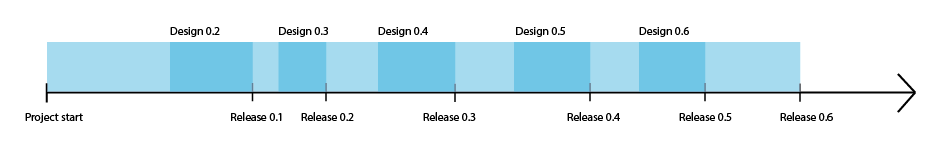
\includegraphics[height=2.6cm]{figs/design-vs-implementation.png}
\caption{How the planning and design phases of the versions were performed in a time line.}
\label{figs:design-implementation}
\end{figure}


\subsubsection{Requirements}
In this project the base for the functional requirements of the version are described in user stories as is a method borrowed from Scrum in the format of Mike Cohn.\cite{scrum-user-stories} The project chose to use user stories for this purpose because the stories detects the needs of the user and makes the requirements user oriented.

At the end of the project when the development process was ended with creating a requirement document representing the functional requirements based on the current product and the demands from the customer in terms of uptime of the server and similar nonfunctional requirements. The nonfunctional requirements were also created continuously, but those requirements were often specified by the customer of the project.

\subsubsection{Prototypes and usability testing}
For all the early versions of the product (0.1 - 0.5) a paper prototype was created  to illustrate the functionality and possible designs. There were created different types of paper prototypes. The first were generic phones with little color whilst the later versions were operative system specific paper prototypes with design features. 

The idea of the paper prototypes were to get a product out to the users as fast as possible and get their reaction and feedback. The paper prototypes were created after the initial assumption and based on the user stories defined to answer the questions created from the assumption. The usability tests with the paper prototypes were conducted at the \gls{NTNU}, mainly on students. 

In addition to the paper prototypes some movies were created to illustrate the application’s functionality before the functionality was implemented. This technique is described in the version 0.1 and 0.2 where there were released movies. 

\subsection{Assumptions and questions}
Assumptions are a key feature of The Lean Startup methodology. At the beginning of each version the team have made a basic assumption. In the early versions this was leap-of-faith assumptions because there were no feedback to use as basis for the assumption. However as the project evolved the assumptions were based on feedback from surveys and the customer. 

The assumption in the Lean Startup Methodology are defined as what the startup believe is true about the users of the product being developed. \cite{lean-startup} In this project there were a lot of assumptions about the users that were examined during the iterations. Each assumption generated a lot of questions about the users. To answer these questions and in that way get an acknowledgement about the assumptions were the goal of each iteration. A list of the assumptions for each version is in table \ref{assumptions}. 

\begin{table}[]
\centering
\begin{tabular}{|L{2cm}|L{11cm}|}
\hline
Version & Assumption \\
\hline
\centering 0.1 & Smoke Test: Are there enough people interested in our product? \\
\hline
\centering 0.2 & Users want to add their books using a barcode scanner \\
\hline
\centering 0.3 & Users want to borrow books and be able to keep track of who has borrowed the book and who they have borrowed the book from \\
\hline
\centering 0.4 & Users wants a group functionality to organize what books they are interested in \\
\hline
\centering 0.5 & Users want to be able to search for book by text \\ 
\hline
\centering 0.6 & Users want to be able to authorize who can join their groups
\\\hline
\end{tabular}
\caption{Assumptions for each version}
\label{assumptions}
\end{table}

\subsection{Feedback}
\label{feedback}
The Lean Startup has a lot of techniques that can be used to get different types of feedback from the user. The most important feedback is the one you get from the actual users according to Eric Ries’ The Lean Startup. In this project Mixpanel was used to measure the users use. At the start of the implementation of a version the team decided what baseline metrics should be used to measure the users use. In Mixpanel you can track any event you wish and add properties to that event for extra information. A table of all the tracked events can be found in table \ref{tab:mixpanel_table}.

There were not a lot of users in the early versions of the application, which entailed that it would be a little difficult to get some real user data other than some users from Netlight. As a consequence of this in addition to  the time limit of the project and continuous development the team focused on the feedback from the customer and the indications from the users until the last version. When the final version was released, what the customer ment was a minimal viable product for Netlight, the real user analysis could start. Unfortunately there is not much to do with the feedback for this report other than to make suggestions for further work.
\begin{table}[]
\centering
\begin{tabular}{|L{2cm}|L{3cm}|L{7cm}|}
\hline
Version & Event name & Comments \\
0.2 & AppLaunced & An event triggered by the launch of the application \\\hline
 & BookAdded & After the user has scanned a book and choose to add it \\\hline
 & BookRemoved & When a user choose to remove a book from their personal shelf \\\hline
 & BookScanned & When a book is scanned using the bar code scanner \\\hline
0.3 & BorrowBook & When a user borrows a book \\\hline
 & ReturnBook & When a user returns a book \\\hline
0.4 & CreateCrowd & When a user creates a crowd \\\hline
 & AddMember & When a user adds a member to a crowd \\\hline
 & LeaveCrowd & When a user leaved a crowd \\\hline
0.5 & BookSearch(Search) & When a user search for a book. Includes the search as property \\\hline
 & SwitchedFilter & When the user switched between "All books" and "In my groups". The search starts on "In my groups"
\\\hline
\end{tabular}

\caption{Mixpanel tracking of events}
\label{tab:mixpanel_table}

\end{table}  

\subsection{Retrospective meetings}
\label{retrospective-intro}
At the end of each version the team had an internal retrospective meeting based on the Scrum standard for retrospective meetings.\cite{scrum-retrospective}  In the first versions the meeting was taken as a round around the table where each member stated what they thought went well in the version and what they thought could be improved to the next. After two versions it was clear that the team members had difficulties with coming up with feedback on the spot, so the procedure was changed. 

From version 0.3 the points were written down on notes instead of all the team members speaking out loud. The retrospective meeting started with all team members writing down at least three positive aspects of the version, and three point of improvement on sticky notes. Then all of these were put up on a white board and read out loud. If someone disagreed they could say it out loud and the team would discuss whether it was correct. After all the improvement points were read through the team agreed upon two-three points they should focus on improving for the next version.

With the new type of retrospective meeting the team got a clearer vision of what was working well, both within the team and in the implementation. It also had a positive effect from getting the team members to agreeing upon common goals and made it easier to correct someone if they did not follow what they had promised.

\subsection{A generic example of a version}
\label{generic-example}
This section describes how a typical version iteration is done in this performed. 

\subsubsection{Assumption and questions}
At the beginning of the iteration, usually before the previous version is released, the team gathers and decides on an assumption that will be tested in the version. Based on that assumption some questions are generated. These questions are created based on what is needed to be learned to determine if the assumption is correct. 

\subsubsection{Planning and design}
After the questions are created the team decides what methods will be used to get answers to those questions. It is usually some method that does not require a lot of time, like a prototype or a survey to get the initial feedback and decide what the team think the users want. Based on the questions and assumption the team creates user stories to represent the requirements selected for the version.
After discussing the possible ways those stories can be implemented and drawing some sketches on the whiteboard the team agrees upon a design of the functionality and a paper prototype is created for initial testing of functionality and design. 

\subsubsection{Implementation}
When the feedback from the initial prototype is done, the development teams start to implement the functionality based on the prototype. The Android team develops the Android application and publish the application on Google Play as soon as it is done. The iOS team develops the iOS application and puts it up for review in iTunes Connect.
The application is published in beta mode so registered users can download the application in TestFlight after the review. The backend team updated the API to support the new requests needed for the version and updates swagger in parallel. The changes are then uploaded to Heroku so the clients can use the new functionality. 

\subsubsection{Feedback}
When the applications are released Mixpanel is used to acquire feedback from the users. The feedback from the customer who is using the application is also taken into consideration. If the team learns that the users do not want the new feature that feature will not be a focus in the next version. If it seems that the users approve of it, and maybe want something more that will be the main focus. In the interest of our customer there are some key features that needs to be implemented in the application, but to which extent and in what manner is up to the feedback received from users.

\subsubsection{Review and retrospective}
After the feedback is received and the new version is released the team meets up and discuss the feedback received. As mentioned in section \ref{feedback} it was a problem to receive enough feedback to be sure about what the users wanted, but the team used the feedback they got and generated new assumption.

In addition to learning about the user’s needs in the application the team has a retrospective meeting after the version is released. When the focus points of the next version has been selected the iteration is done. 

\section{Version 0.1}
The first version of this project included learning about the \gls{LSU} methodology and development of the application. It produced three movies in two iterations where the first movie included several user stories and the other two movies each represented a selected user story. The duration of this version was almost four weeks, but it included a lot of the ground work needed for the team to be able to develop an application and follow the lean startup methodology.

\subsection{Assumption}
The goal of this release was making a video explaining what the team assumed the purpose of the product would be. This was done to conduct a so called smoke test where the video was created to learn if it was enough users interested in the product.

\subsection{Planning and design}
After the first meeting where the team had been introduced to the customer and the idea of the product all the members  had to draw a sketch of what they thought the application would function. There had been some differences in the perception of the functionality, but at the second team meeting the different sketches were discussed and the team agreed upon what was thought to be the most important features of the application. 

With these features as a basis the initial \gls{mockup} of the application was created. It was decided that the most resource efficient manner of doing a smoke test was to make a simple video explaining the product. The \gls{mockup} was used to represent the potential application in the first demonstration movie. 

The team decided to gather the feedback from the movie using a survey on the website, and unstructured interviews. In the survey, users could add their email address in order to receive updates and become beta testers. 


From the feedback received of the first movie, the team learned that three different examples of use in one movie could seem confusing for the people who had never heard of the product. Due to this response, the team reconsidered the movie and decided decided that the users were likely to be students and companies. Based on this decision two new movies was created. Each represented one of these scenarios of use. These target groups were also available for contact through Netlight and fellow students. The two new movies were released on the same web page with an updated version of the feedback survey. 

In parallel with making the demonstration videos, it was agreed that the mobile teams should start creating the basis for the applications, and that the backend should start building the initial \gls{API} and consider different database options.


\subsection{Development}
An information video was the main focus during this first version, but in order to avoid spending unnecessary resources, the development on both client platforms and the backend was initiated.

\subsubsection{First demonstration movie} 
The first video was made using Balsamiq \cite{balsamiq} where the touches in the application was represented by a pointer. The movie told three stories to present possible use of the application while showing the functionality. The voice was recorded using Audacity. 

The first scenario in the movie was a woman named Jane who work at a company with a lot of books for collective use. It was then presented how the company could keep track of all these books using the new application.

The second scenario was Joseph who owns a lot of books. He likes to share them with his friends and can now, with the help of the application always have an overview of who has which book. 

The third scenario was Emma the student who is in a colloquium where the students like to share the course litterature among each other. In this scenario the crowd functionality is represented to show how she can see which books the colloquium has to offer.

The movie can be watch at \url{https://www.youtube.com/watch?v=7KbctbCdvvU} and a snapshot is shown in figure \ref{fig:information-film-01}.
\begin{figure}
\centering
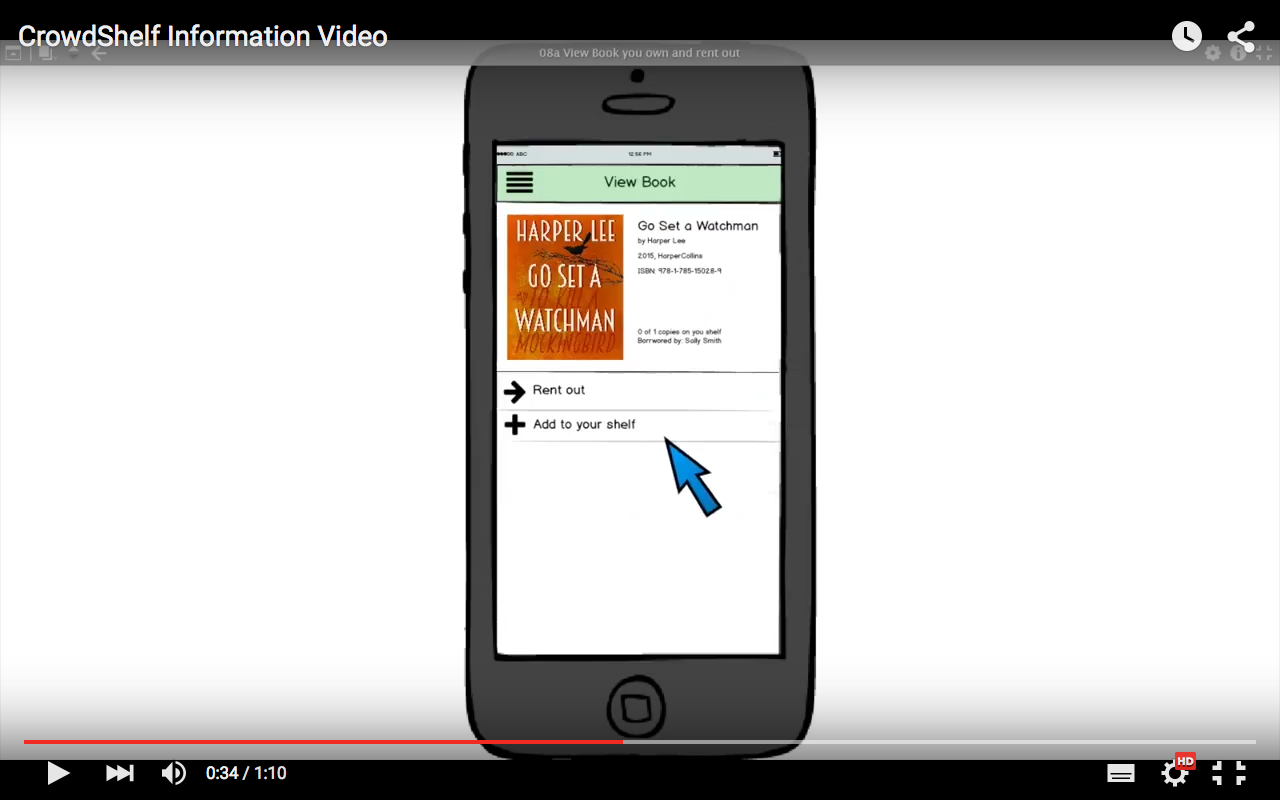
\includegraphics[height=5cm]{figs/v01/FirstInformationMovieBook.png}
\caption{Shot from the first demonstration movie}
\label{fig:information-film-01}
\end{figure}

\subsubsection{The student and company movies} 
The two movies that represented the student and company example respectively was created using Adobe Edge Animate to achieve a more professional look. 

The movie that represent the student example brought up the issue of buying expensive new books and that it is preferable maybe to borrow the books from fellow students. It then shows the students creating a crowd and adding other members. Afterwards the movie shows that the student finds out who has the desired book using the application and then seeks her out, scan the book with the application and borrow it. 

In the company example movie the focus is on the value of the employees competence and how that knowledge often is obtained by reading books. The problem occurs when the company’s shelf becomes empty and the employees can not find the books.The movie then shows how the company can create a crowd so that they and the employees can know where the books are at all times.

The videos were shared on Youtube and on the project's web site. They can be watched at \url{https://www.youtube.com/watch?v=yj0NNimKgIw} and \url{https://www.youtube.com/watch?v=6Nedobb4eZ0}. Snapshots from the movies are in figure \ref{fig:student-example} and figure \ref{fig:company-example}
\begin{figure}
\centering
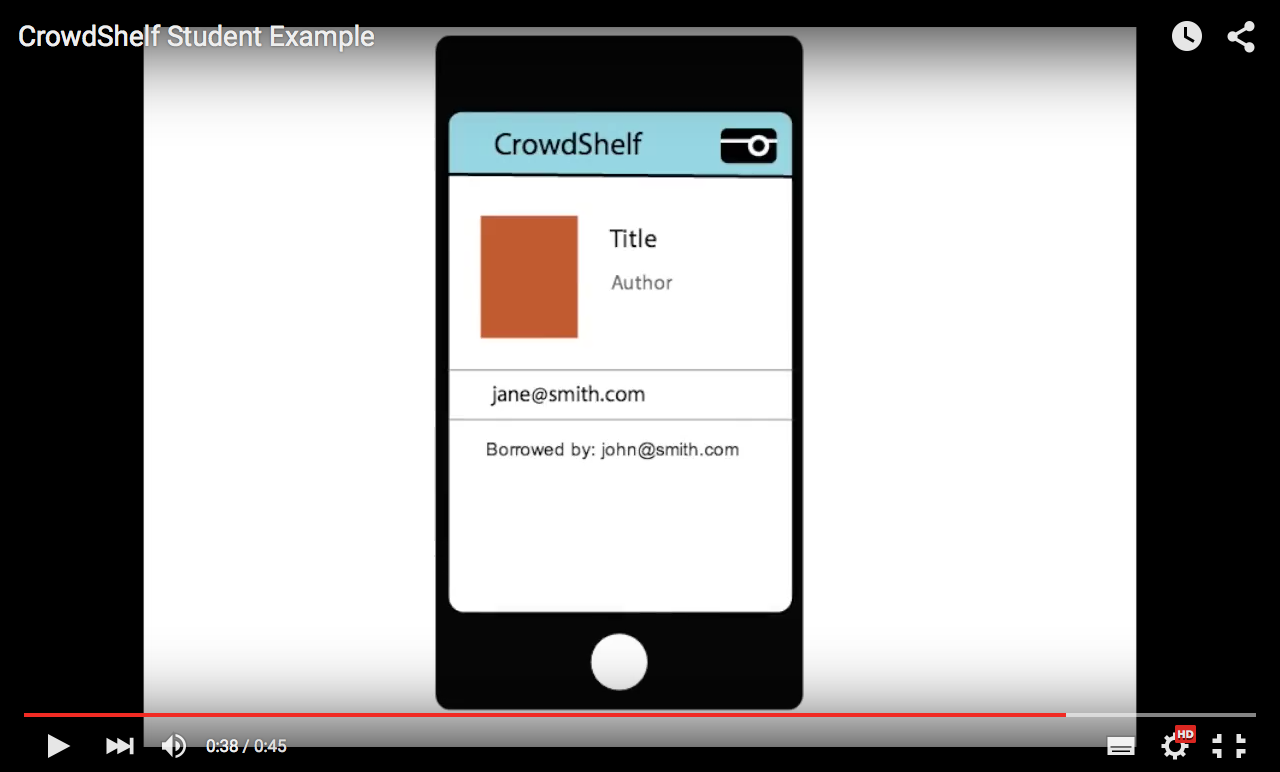
\includegraphics[height=5cm]{figs/v01/InfoMovieStudent2.png}
\caption{Shot from the student example demonstration movie}
\label{fig:student-example}
\end{figure}

\begin{figure}
\centering
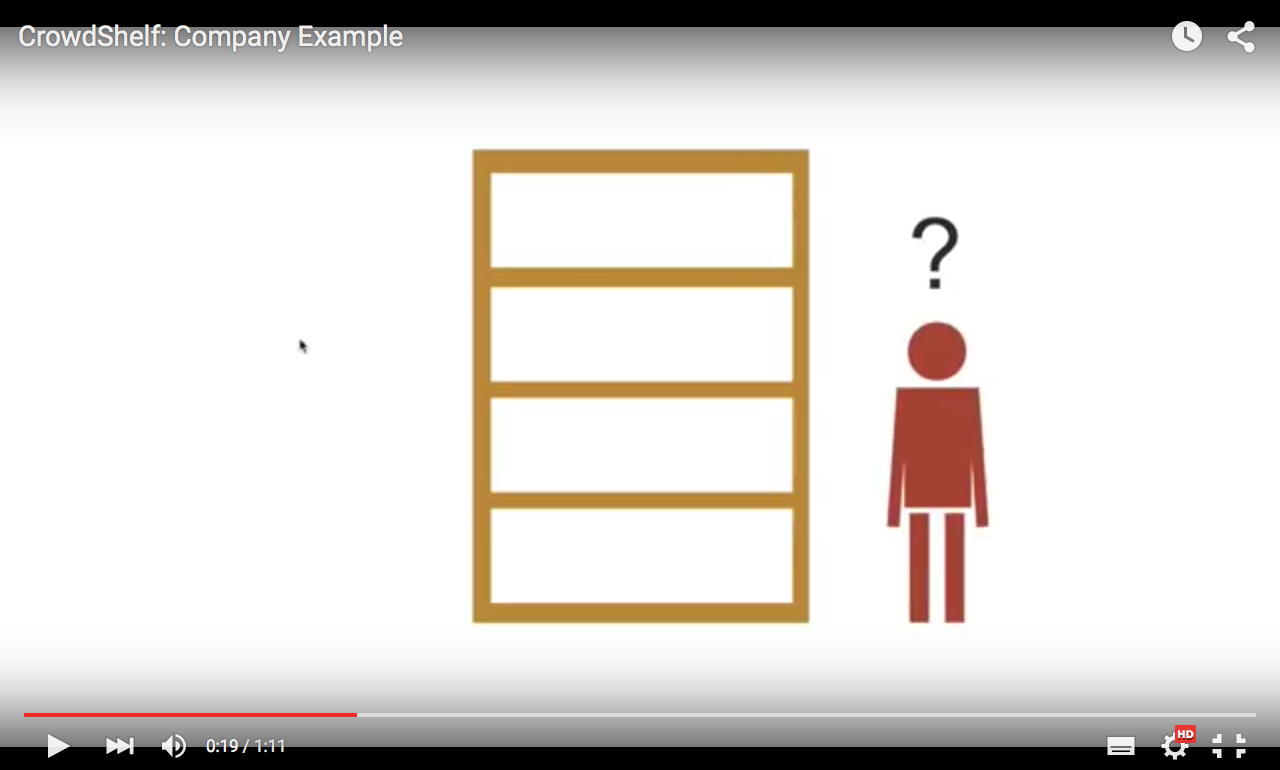
\includegraphics[height=5cm]{figs/v01/InfoMovieCompany1.png}
\caption{Shot from the company example demonstration movie}
\label{fig:company-example}
\end{figure}

\subsubsection{Android}
The Android team encountered a few challenges due to limited experience with the platform, and therefore the development took more time than anticipated. The lack of experience with Android development caused the Android team to spend first iteration learning about the Android platform. During this iteration the team watched videos and read tutorials explaining different aspects of the Android platforms, such as how to use tools such as Android Studio and how to test the applications created on a physical Android device.\cite{android-studios}

By end of the iteration the Android team was able to use the camera of a device as a barcode scanner, and also track usage using a third party tracking service called Mixpanel.\cite{mixpanel}

\subsubsection{iOS}
%A lot more information. Tell how everything was done!
During the first iteration, the iOS team started setting up the project by adding Cocoapods and including all necessary libraries. \cite{cocoapods} These included the networking library Alamofire, the database library Realm, and the barcode scanner library MTBBarcodeScanner. \cite{alamofire}\cite{realm}\cite{mtbbarcodescanner} Alamofire and Realm enables effortless parsing and deserialization of \gls{JSON} responses, and greately reduces the complexity of the interaction with external services.  \cite{json}

The team also did some research to determine the easiest way to distribute and test beta versions of the application. There were many tools available, but only Apple's proprietary TestFlight enabled distribution to external testers without manually registering multiple devices on the Apple Developer Program license. \cite{testflight}\cite{apple-developer-program} Thus TestFlight became the obvious choice.

After the necessary tools were selected, the development of the application could begin. The application would have a data-driven approach, and therefore the first task was to create the data models necessary for the application. \cite{data-driven-programming} These included User, Book, and BookInformation classes. The User contains information such as \gls{ID}, username, email, and name. The Book object contains information from the CrowdShelf backend about the books \gls{ID}, \gls{ISBN}, the owner, who the book is rented to, and whether it is currently available for rent. The book information contains general information about a book retrieved from a third party information provider such as title, authors, and summary. For this version only Google Books \gls{API} was added as an endpoint for information, but the system was designed to easily handle additional endpoints at a later time.\cite{google-books-api}

All user interfaces were designed using the Xcode \gls{IDE}'s built in user interface builder, and were assigned a view controller. For this version, only a simple book view, shelf view and scanner view were implemented.


\subsubsection{Backend}
The first iteration of the \gls{backend} included quite a lot of implementation and code. First of all, the backend team decided on what to build the \gls{backend} with, which was the document-oriented database system MongoDB, and NodeJS with ExpressJS. \cite{mongodb}\cite{node-about}\cite{express} Then the team set up the project, and created a readme-file with installation instructions, and a outline of data model and \gls{API}. This was the only documentation for the \gls{API} for a few versions. The readme-file was shared with  the other development teams, so they knew what they would be working with.

Then the team started coding, by setting up some models for the entities books, users and crowds. These models are modules that present an \gls{API} to other modules to find, update and insert documents into the database. The team also set up a router with the routes, and controllers for the entities. The controllers hold the actual logic surrounding each request. 

The team also set up an environment for which the client applications could use the \gls{API}. This was done with Heroku, together with MongoLab.\cite{heroku}\cite{mongolab} Heroku hosted the server, under the domains \url{http://crowdshelf.herokuapp.com} and \url{http://crowdshelf-dev.herokuapp.com}, while MongoLab held two separte databases for us. The first domain served the code from the \code{master}-\gls{branch} on GithHub, while the second served the code from the development \gls{branch}. For each iteration the team decided to merge the development \gls{branch} into the master \gls{branch}, so that the team had a stable version of the server somewhere, while the team developed new features. Heroku pulled changed from GitHub and restarted the server automatically when something was changed on either branches. This structure is still in place, even though our the main location for the stable version of the server was changed in a later iteration. 

By setting up the server, database and making it available to the development teams working on the client application, the backend team completed its requirements for this iteration.

\subsection{Feedback}
The feedback received from the the initial demonstration movie is mentioned in the planning phase. In other words the vital feedback was collected from the second version of the smoke test where the stories to show use of the application emerged with new clarity. The responses was received through the survey shown in figure \ref{fig:0.1-survey} 

Although the feedback acquired from the survey was positive there were only fifteen responses, which is not sufficient to use as the basis for continued development. Additionally, not all of the responses contained an e-mail address so there was not possible for the team to give the, information about updates. The answers from the survey can be are shown in table \ref{feedback-v1}.

In spite these results, the customer representative stated that the solution conveyed in the videos adequately reflected his needs as a customer. He therefore allowed the development to proceed with the functionality shown in the movies as the concept of the application.

\begin{figure}
\centering
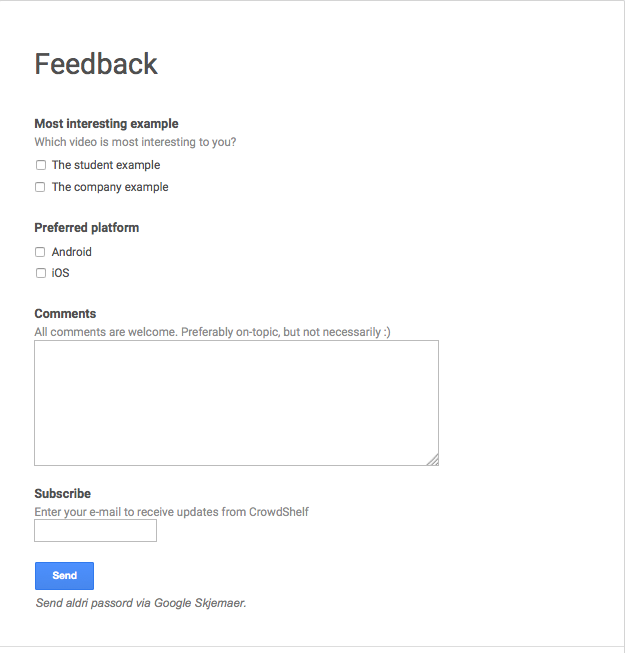
\includegraphics[height=7cm]{figs/v01/01Survey.png}
\caption{The survey from the web page}
\label{fig:0.1-survey}
\end{figure}


\begin{table}[]
\centering
\begin{tabular}{|L{2cm}|L{4.5cm}|L{2cm}|L{2.5cm}|L{3cm}|}
\hline
\textbf{Timestamp} & \textbf{E-mail} & \textbf{Preferred platform} & \textbf{Preferred example} & \textbf{Comments} \\
 \hline

07.09.2015 & jacke.andersson@gmail.com &iOS	  & The company example & - \\
 \hline
 09.09.2015 &  fredsg@gmail.com& Android & The student example  & - \\
 \hline
09.09.2015 & - & Android, iOS  & Both & - \\
 \hline
09.09.2015 & - & Android & The company example & - \\
 \hline
09.09.2015 & - & Android & The student example & Interessting movie! Maybe information about the book standard? \\
 \hline
09.09.2015 &-  & Android & The student example & Nice video, seems like a simple and good app \\
 \hline
09.09.2015 & annakastet@gmail.com & Android & Both & - \\
 \hline
09.09.2015 & peder.kongelf@gmail.com & iOS	 & The company example & More focus on integration with amazon and recommended books \\
 \hline
09.09.2015 &-  & iOS	 & The student example & - \\
 \hline
 10.09.2015 & - & iOS	 & The student example & - \\
 \hline
12.09.2015 & roald40@hotmail.com & Android & The student example & Splendid! Looks very helpful for students as myself. I like it :)  \\
 \hline
20.09.2015 & -& Android & The student example & Top nice app you guys \\
 \hline
05.10.2015 & - & Android & The student example & -\\
 \hline
05.10.2015 & martinwidding@hotmail.com & Android & The company example & Good brand name, cool idea. The Company example is both more appealing, and you do not feel "talked down to" (as in dumbed down) \\
 \hline
16.10.2015 & - & iOS	 & The company example & - \\
 \hline

 
\end{tabular}
\caption{Feedback from survey}
\label{feedback-v1}
\end{table}

\subsection{Version progress}
During this version a lot of tasks were completed to create the foundation of the application. There were administrative tasks that had to be done and new knowledge to be acquired. A figure of the task progression is shown in figure  \ref{fig:progress-v1}.

\begin{figure}
\centering
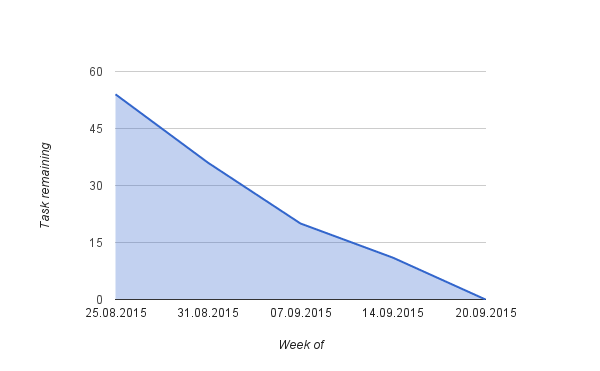
\includegraphics[height=10cm]{figs/v01/progressv1.png}
\caption{Task progression version 0.1}
\label{fig:progress-v1}
\end{figure}


As illustrated in the figure the progress was very good in the first two weeks, while the progress slowed down in the third week. There are two reasons to explain that freeze. The first is that many of the tasks were not in context to implementation which means that the team knew how to complete them. The release note that explains the tasks done in this version is shown in appendix \ref{app:release-note-1}.

As week three was completed the team had encountered some problems which is the other reason. The setback occurred when the implementation had begun and the \gls{API} had to be rewritten to follow rest standard. In addition the Android team learned that they had to remake the structure. 

By the fourth week the project moved forward after the setback by not rushing the implementation and taking the time to learn the different structures of the platforms used for implementation. 

To continuously describe the process to the customer and supervisor the team wrote a blog. The blog posts that were written in this version are shown in figure \ref{fig:week-one}-\ref{fig:week-four}

\newpage
\begin{figure}
\centering
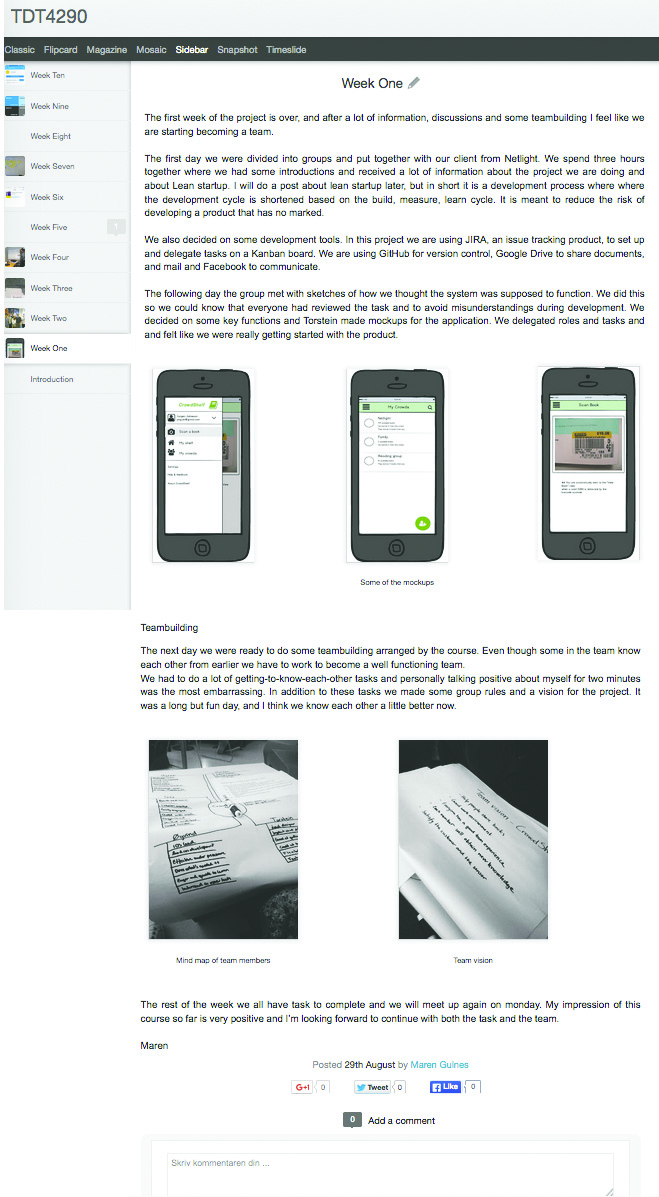
\includegraphics[height=22cm]{figs/v01/WeekOne.jpg}
\caption{Blog post from week 35}
\label{fig:week-one}
\end{figure}

\begin{figure}
\centering
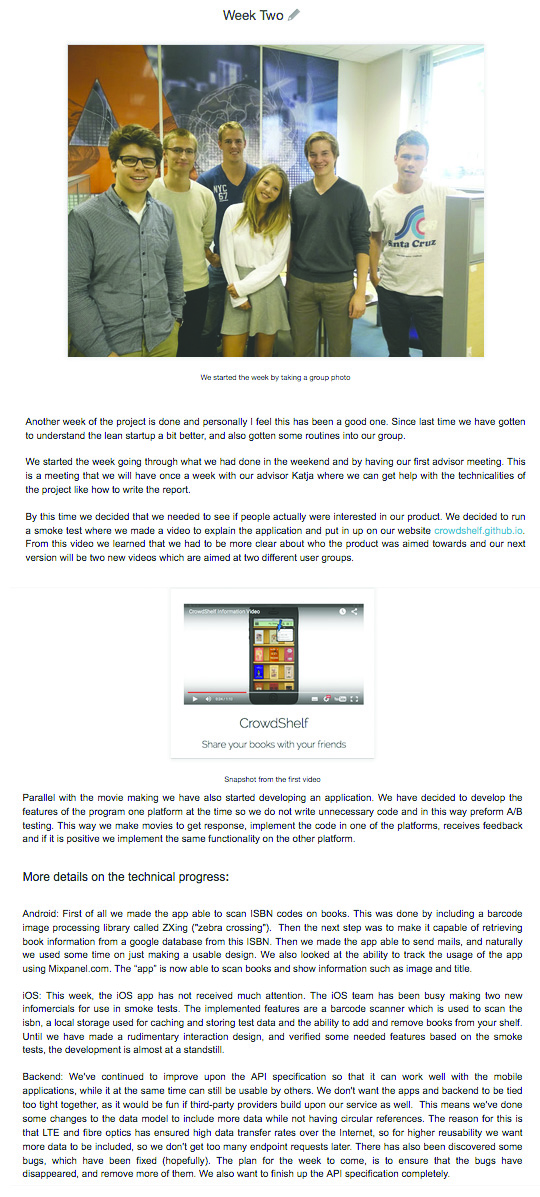
\includegraphics[height=22cm]{figs/v01/WeekTwo.jpg}
\caption{Blog post from week 36}
\label{fig:week-two}
\end{figure}

\begin{figure}
\centering
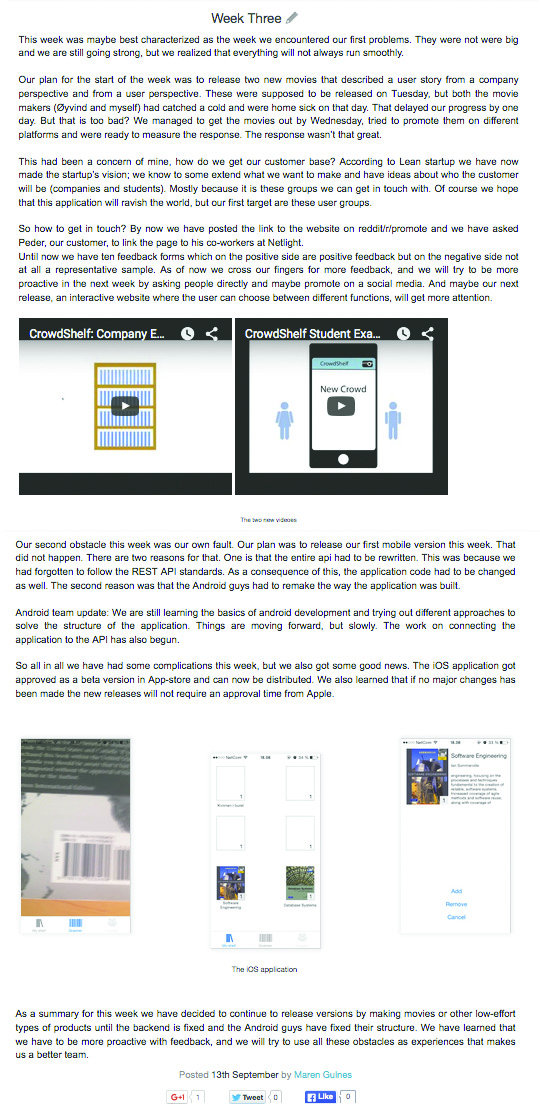
\includegraphics[height=22cm]{figs/v01/WeekThree.jpg}
\caption{Blog post from week 37}
\label{fig:week-three}
\end{figure}

\begin{figure}
\centering
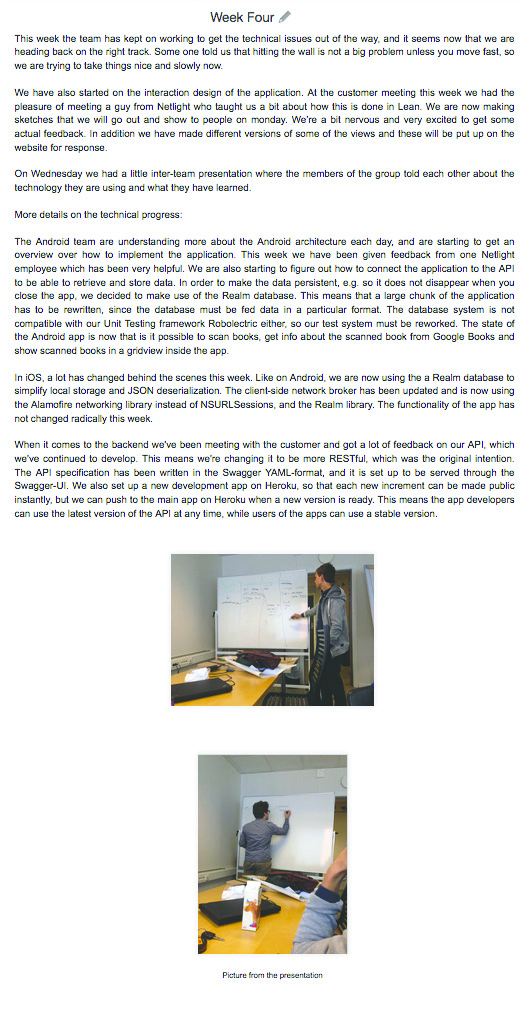
\includegraphics[height=22cm]{figs/v01/WeekFour.jpg}
\caption{Blog post from week 38}
\label{fig:week-four}
\end{figure}

\newpage
\subsection{Review and Retrospective}

In this project the review by the customer happens every week where in a customer meeting where the team presents what is new from the last meeting. The customer contact was very pleased in the beginning of the version with the effort put in the movies and how the team learned about the Lean Startup. He also came with comments on how he wanted the representations in the meetings to be done. From the fourth meeting he requested a demonstration video of the applications each week. It was also he who requested the \gls{API} to follow the REST standards. 

At the end of the version the team had a retrospective meeting where the team members talked about what went well and what could be improved in the iteration. Positive in the version was the interaction in the team. All the team members felt that the communication was good, and that everyone worked the hours they were supposed to. On the less positive side was how the structure of the iteration had been performed. There should be clearer common goals, and more focus on following the Lean Startup.

The three subteams all produced some basic software for the product, and became more familiar with the technologies that were going to be used. There were many lessons to be learned, but by the end of this version the team has achieved a greater understanding of how this project will be structured, and the about the technical issues in their domain.  


\subsection{Summary}
At the beginning of this first version, the team had did not know what the features of the finished product would be. Through a smoke test with videos and surveys, and discussions with the customer representative, the concept for the application has been decided. The team will now focus on deciding what functionality is most important in the application to show how the product will function.

Allowing the to work on their respective tasks for the user stories in parallel with the video proved to be a good decision. It enabled the the clients and server to be synchronized in future iterations.



% Version 0.2
\section{Version 0.2}

The goal of this iteration and version was to create a \gls{MVP}. This \gls{MVP} contained what the team thought was the most important features of the application. It was done by creating an assumption with questions to be answered, select the the user stories needed to support that feature and measure the use.

\subsection{Assumption and questions}
The assumption to be confirmed for this iteration was
“Users want to add their books to the application using a barcode scanner”.

To confirm this assumption the team generated questions that should be answered to do so.
\begin{enumerate}
    \item Is it easy for the user to find a book’s barcode?
    \item Do the user think it is simple to scan a barcode?
\end{enumerate}


\subsection{Planning and design}
With the assumption and questions as basis, the team had to decide how to measure the result, and what user stories should be selected to be able to test the questions. After meeting with employees from Netlight, it was decided that user tests with paper prototypes was the best way to get an indication on whether our assumption was correct, and verify that our design was user friendly and intuitive. The user stories selected are described in section \ref{user-stories-v2}. 

An employee at Netlight named Magnus Skaalsveen had a session with the team where he taught the use of Lean UX.\cite{lean-ux} The goal of Lean UX is to create low-fidelity prototypes, like a whiteboard sketch or a paper prototype which take shot time to iterate upon. With these levels of design the build-measure-learn cycle can be executed more rapidly.  

At the meeting the team and Skaalsveen did a couple of sketches on a whiteboard to generate the design of the selected functionality. By doing so the team learned that there were a lot of points where the idea of the application still was unclear, and that by drawing in that manner created a good space to discuss those issues. 

Based on the sketches created on the whiteboard, paper prototypes were created to perform usability test where the goal was get indications on both questions and design.
The usability tests were performed at the university, and in the fashion of hallway tests executed on randomly selected students. Students were targeted because they were a part of the target audience and easy to come in contact with. 

 The tests would consist of a set of tasks the user would perform on paper prototypes of the application. The test team consisted of two team members. One acted as test leader and system while the other documented all the users feedback, hesitations, problems and other relevant information. After the test, a short unstructured interview was performed to ask what the user thought about the general idea behind the application. 

Prototypes created to support the selected user stories are shown in figure \ref{fig:user-story-prototype-v2-1} and \ref{fig:user-story-prototype-v2-2}.
In addition there were some design alternatives associated with user story number \ref{02-user-story-see-books-in-shelf}, the shelf view. The alternatives are shown in figure \ref{fig:design-alternatives-v2}. After the usability tests the first alternative was chosen as the design for the application. 

\begin{figure}
\centering
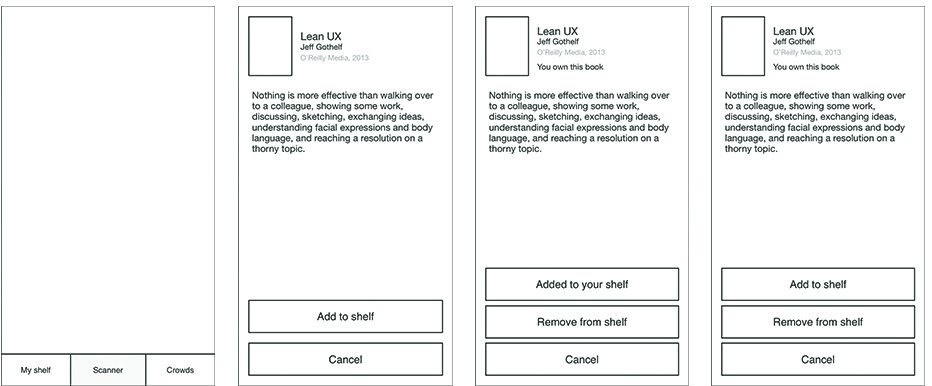
\includegraphics[height=5cm]{figs/v02/userstory-v2-1.jpg}
\caption{Paper prototype from the user stories of adding a book and scanning the barcode. }
\label{fig:user-story-prototype-v2-1}
\end{figure}

\begin{figure}
\centering
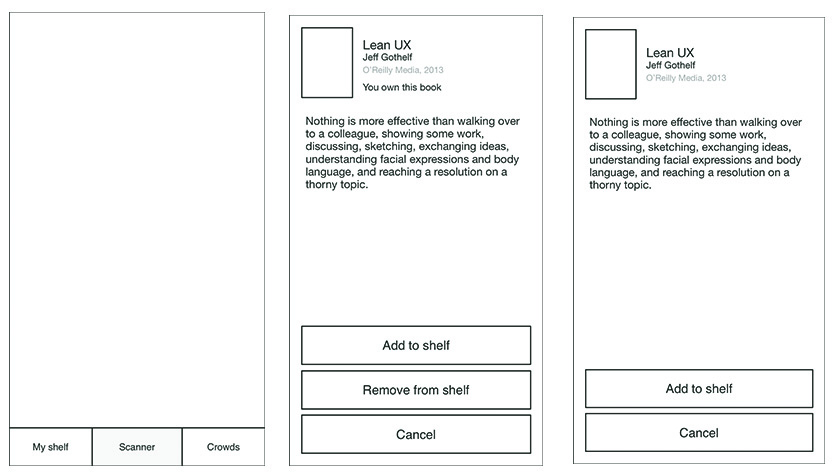
\includegraphics[height=5cm]{figs/v02/userstory-v2-2.jpg}
\caption{Paper prototype from the user stories of removing a book and scanning the barcode }
\label{fig:user-story-prototype-v2-2}
\end{figure}

\begin{figure}
\centering
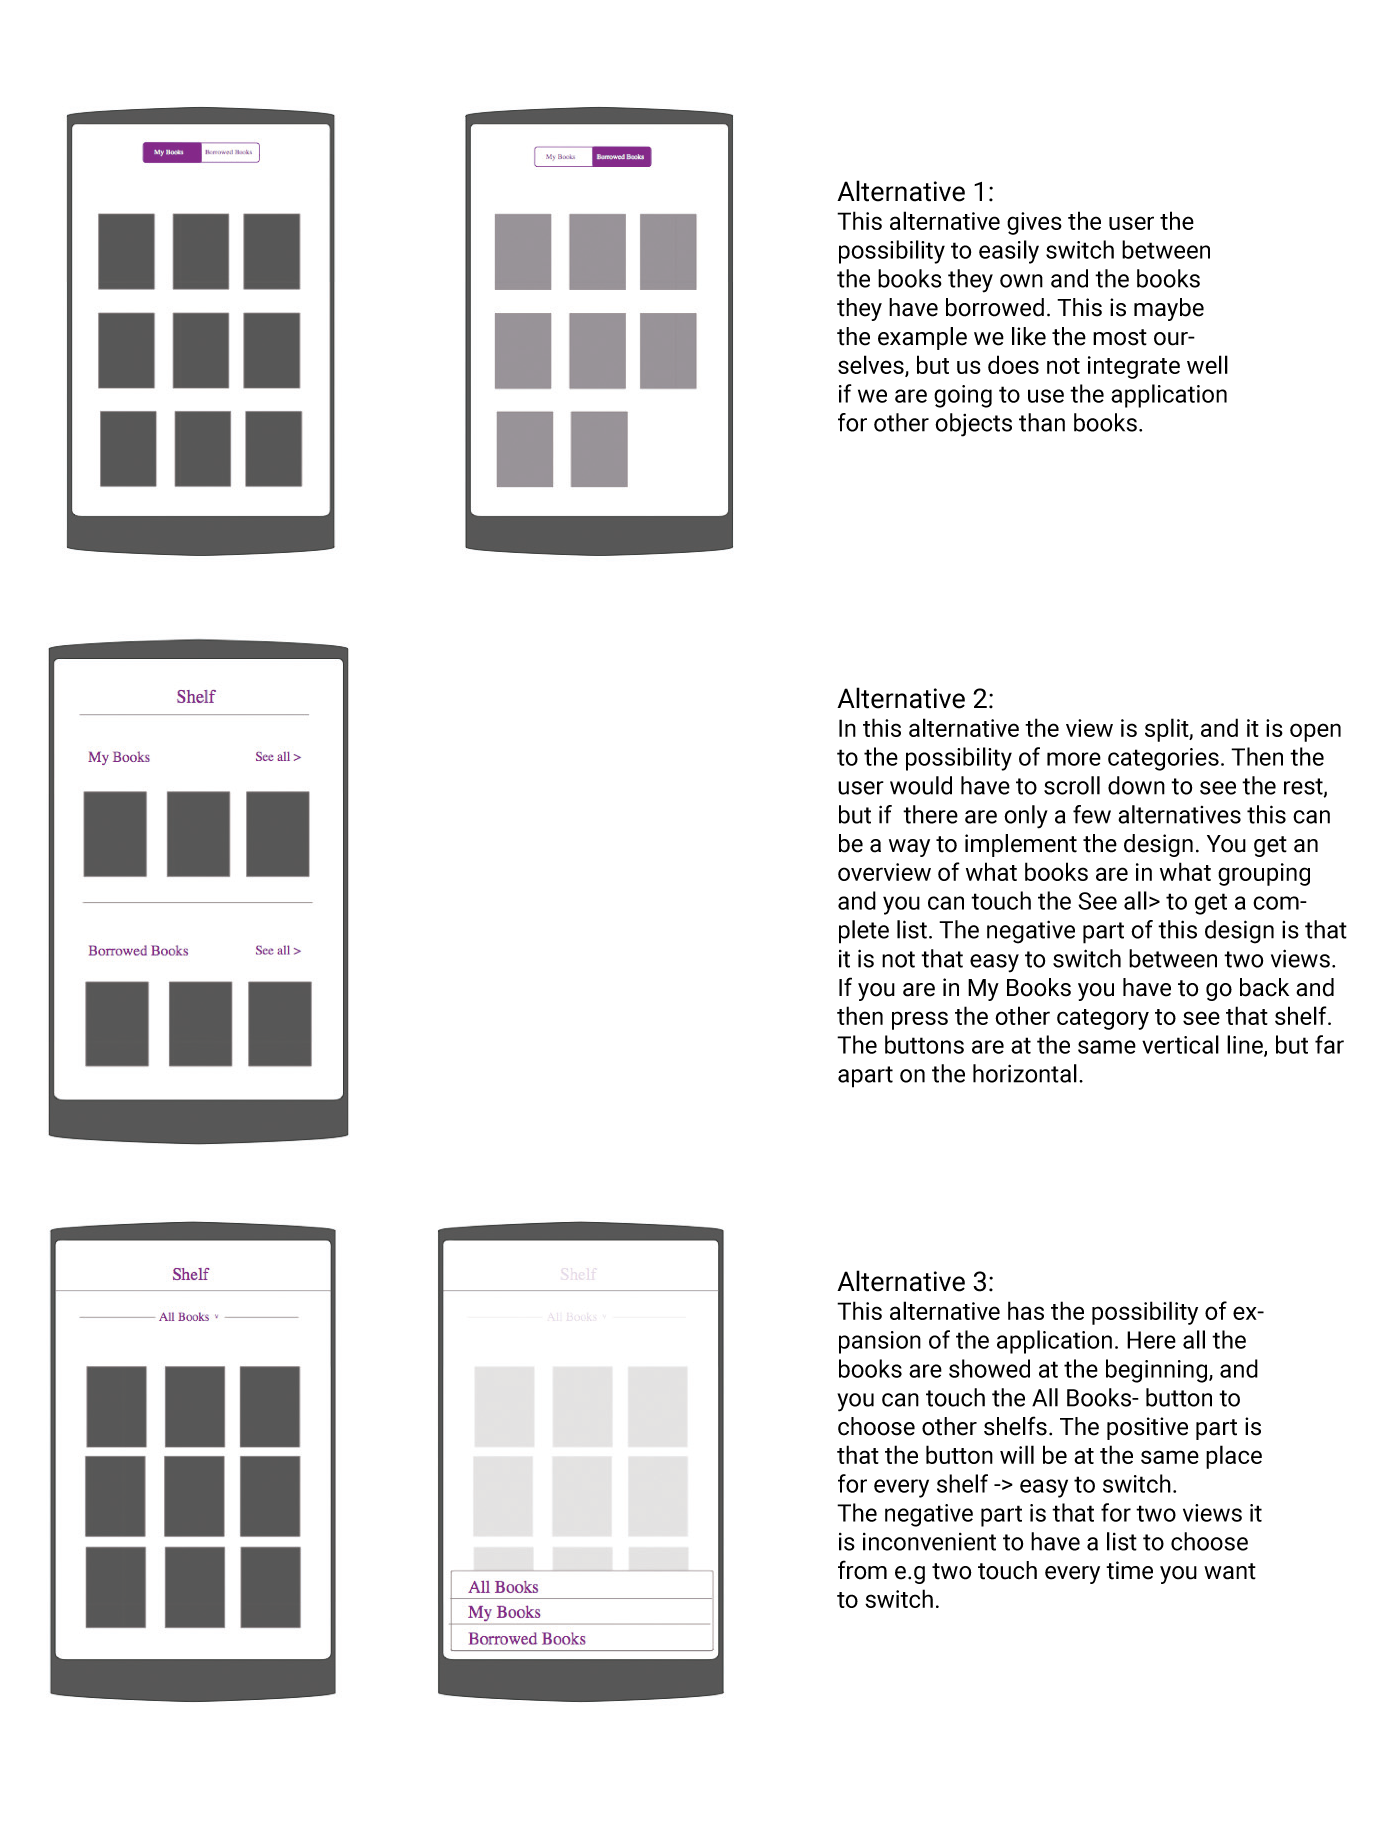
\includegraphics[height=22cm]{figs/v02/design-alternatives.png}
\caption{Design alternatives of the shelf view with argumentation }
\label{fig:design-alternatives-v2}
\end{figure}

\newpage
\subsection{User stories}
\label{user-stories-v2}
This section shows the user stories selected as requirements version 0.2. The stories are selected based on the initial assumption, and what was thought to be the most relevant features to test it. 

\begin{enumerate}
  \item As a user I want to add books to my shelf
  \item As a user I want to remove books from my shelf
  \item As a user I want to see the books in my shelf \label{02-user-story-see-books-in-shelf}
  \item As a user I want to search for books by scanning the barcode 
  
\end{enumerate}


\subsection{Development}
After the paper prototypes were done and had received feedback from users, the client teams started implementing the applications. Based on the user stories derived from the assumption and the prototype testing, the development team had enough information about what should be implemented to start the development. This section explains the implementation performed for this version in detail divided in sections of the subteams. 

\subsubsection{Android}
\begin{description}
    \item[Features] \hfill\\
The first feature the Android team developed for the Android application was the ability to scan a barcode of a book using the camera of an Android device to retrieve the ISBN number of a book. This was done by including a barcode image processing library called ZXing ("zebra crossing").\cite{zxing} The feature to be implemented was to retrieve information from this ISBN. This was done by sending an asynchronous \gls{HTTP} GET message to the Google Books' \gls{API} using the URL "http:www.googleapis.com/books/v1/volumes?q=isbn:", where the ISBN is concatenated to the end of the URL.\cite{http-method-spec} Since the call was asynchronous it could be executed in the background while the application could do other operations. If the Google Books contained information about the book, it would return the information stored in a JSON-object.\cite{json} Then Google's Java library GSON was used to convert the received JSON-object to Java objects.\cite{gson} This allowed the rest of the application to easily access the retrieved information and the team also chose to store this information in a local database called Realm. Realm stored the information locally, which meant that the next time the same information was needed it could be retrieved from Realm instead of performing another asynchronous request to Google Books. Realm, the local database, makes the information accessible to all activities and fragments of the application. Realm worked the same way with information retrieved from our \gls{backend}, where it stored information about books locally. The application also had to update the \gls{backend} when some changes were made, i. e. when a book was added or deleted.\\

\item[Structure] \hfill\\
The first version of the Android application contained many different classes since features such as networking and user interface was implemented. Figure \ref{fig:Android-structure-0.2} shows how the application's activities and fragments interacted. The \code{MainTabbedActivity} is the main activity launched when the application starts for the first time. This activity contains two tabs which are switching between displaying the two fragments \code{UserScreenFragment} and \code{ScannerScreenFragment}. The \code{UserScreenFragment} shows which books the user have stored, and the \code{ScannerScreenFragment} has the ability to scan barcodes using the camera of the device running the application. Information and data such as a barcode number in fragments are sent back to the \code{MainTabbedActivity}, which can start other activities using intents. 

The application communicates with the \gls{backend} and Google Books using a static class called \code{MainController}. This is explained further in chapter \ref{chap:ArchitecturalDescription}. 

\begin{figure}
\centering
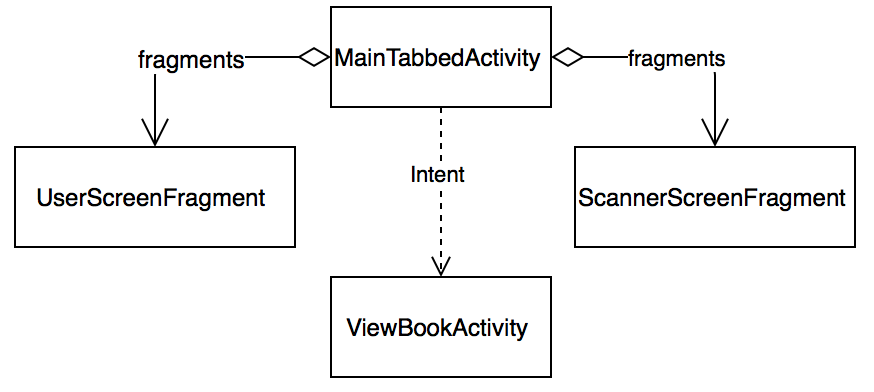
\includegraphics[width = \textwidth]{figs/v02/AndroidStructure02.png}
\caption{The structure of activities and fragments in the Android application in version 0.2}
\label{fig:Android-structure-0.2}
\end{figure}

\item[Design] \hfill\\
When the implementation of the functionality of version 0.2 was almost done, the Android team started looking at the usability of the application. Since none of the team members had much prior experience with Android development, they decided to set the basics of the design before to much code were implemented. The main activity was implemented as a tabbed activity. This made the activity able to have tabs that could be used to change between fragments, in addition to making it possible to swipe between fragments. This gives more possibilities to the design of the application, and the number of tabs could be set to one, to get it back to how it was. But in hindsight the team decided that version 0.2 should probably just be as basic as possible, focusing on implementing features. This would mean some extra work, but also more time to get feedback. Other than the tabbed activity this version was very basic. The elements were just placed somewhere they could be seen and used, but the sizes and relative locations were not important. The activity which shows book information and allows users to remove and delete books is shown in Figure \ref{fig:book-view-v2}.

\begin{figure}
\centering
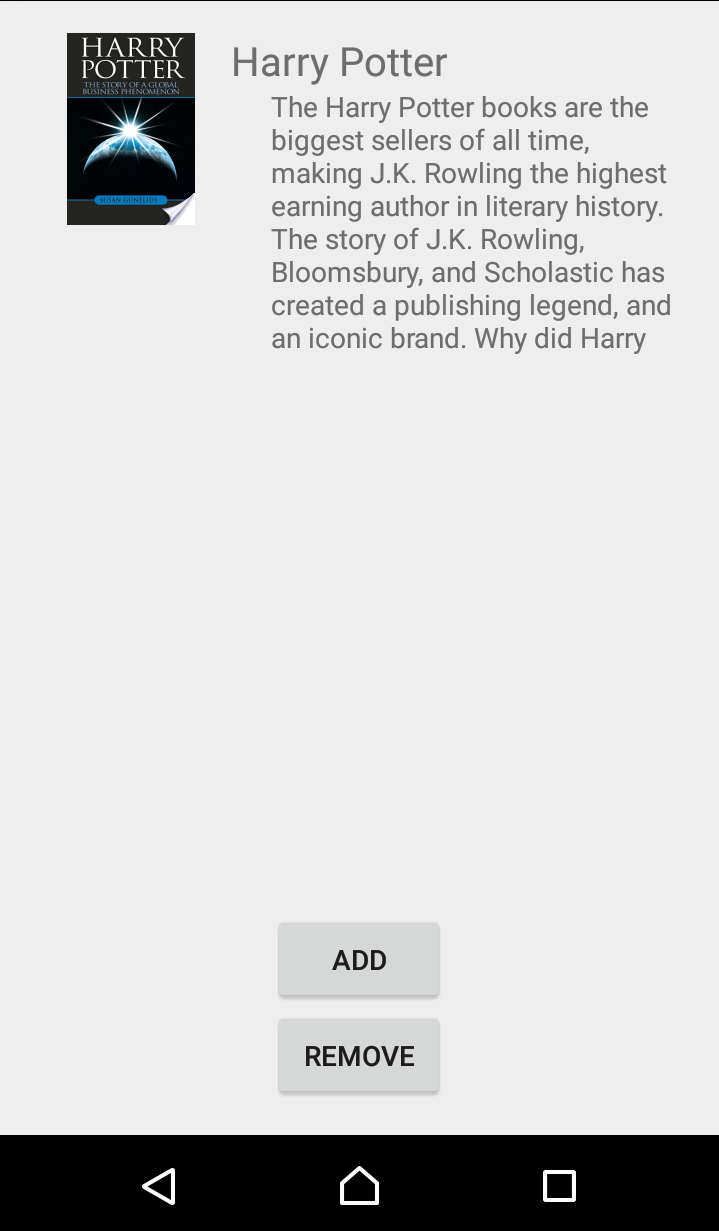
\includegraphics[height=7cm]{figs/v02/bookView02.png}
\caption{The ViewBookActivity showing book information in version 0.2 of the application}
\label{fig:book-view-v2}
\end{figure}

\item[User feedback] \hfill\\
To get feedback about how the users used the application, the analytics tool Mixpanel\cite{mixpanel} was added to the application. Using Mixpanel allowed the application to track specific actions the user performed. In version 0.2 Mixpanel registered each time a user launched the application and when a book was added. See table \ref{tab:mixpanel_table} for a full list of events that got tracked during version 0.2.
\end{description}

\subsubsection{iOS}
\begin{description}
\item[Structure] \hfill\\
This version was essentially a continuation of what the iOS team had been creating during version 0.1. It had been concluded that using the \gls{MVC} architectural pattern in combination with \gls{MVC} was the best approach.\cite{architectural-pattern} As most of the views, controllers and models were already created, the existing implementation only needed some minor changes. 

\item[Features] \hfill\\
The new feature in this release was that the application should communicate with the \gls{backend} when adding and removing books. This lead to the implementation of a new network handler class using the Alamofire library.\cite{alamofire} The network handler provided an interface for asynchronous \gls{HTTP} request for retrieval of information such as book and users. It would first try to parse the response as \gls{JSON}, but if that failed, it would treat the response as raw text. 

\item[Design] \hfill\\
The design used during the usability test was modified based on the feedback from users, and implemented in the application. The basic navigation method was iOS' standard tab bar, and all elements in the view conformed to Apple's Human Interface Guidelines. \cite{human-interface-guidelines} This was to ensure that all users would recognize the function of all elements such as buttons, labels and lists.

\item[User feedback] \hfill\\
In order to receive feedback from actual users about how they used the application, the iOS team integrated Mixpanel.\cite{mixpanel} It was used to track how users scanned books, added books, and removed books from their shelf. This was to be used when measuring the effect of future updates. Increased usage would indicate that the users were enjoying the application more than before the update.
\end{description}

\subsubsection{Backend}
The second iteration of the \gls{backend} was mostly spent improving upon the work from the first one. Everything was up on running, but there was no validation, and limited number of HTTP-response codes returned. In other words the server and \gls{API} was too simple, and the iteration was spent improving upon it. The team rewrote some of the \gls{API} endpoints and the data to be saved and returned, and added more context to responses and request. E.g. the team implemented the use of the HTTP-codes 404 and 422 to indicate that resources weren't present, or that a posted resource was on an invalid format. The team also implemented extensive validation of \gls{JSON}-data that was posted to the server. As a document-oriented database system lets you put anything into it, you have to enforce a data schema in the software code if you want it. This is why the team implemented the library Joi to validate the data. \cite{node-joi-module} This improved the communication with the client development teams.

The team also found that the server wasn't as RESTful as the team wanted it to be. It seems that the team misunderstood some of the aspects of the RESTful standards, which in turn meant that the team read up on it, and redesigned the API. \cite{w3c-rest} The team used the White House standard for RESTful APIs as a template, and used the APIs of GitHub and Twitter as inspiration. \cite{whitehouse-api-standard}\cite{github-api}\cite{twitter-api} Until now the only documentation of the \gls{API} was the readme-file in our project folder, available on GitHub. The latest version of the readme can be read in appendix \ref{app:backend-readme}. The customer wanted us to document the \gls{API} with Swagger, a tool to create an interface for your API, so that developers can explore it and easier understand it. \cite{swagger} First the team explored how the team could make the services already made self-documenting, but found that the tools to make an already exciting solution in Node self-documented with Swagger was hard. Instead the team wrote a Swagger specification with the Swagger Editor, that could be viewed in the Swagger UI. \cite{swagger-editor}\cite{swagger-ui} The Swagger-file written in the Swagger Editor was simply a \gls{YAML}-file on the format that the Swagger-UI needs. A screenshot of how the Swagger documentation looks in the Swagger UI, can be seen in figure \ref{fig:02swagger-docs}

The iteration also involved a lot of bug fixing, bugs that the client development teams reported over the course of the iteration.

\begin{figure}
\centering
\begin{subfigure}{\textwidth}
  \centering
  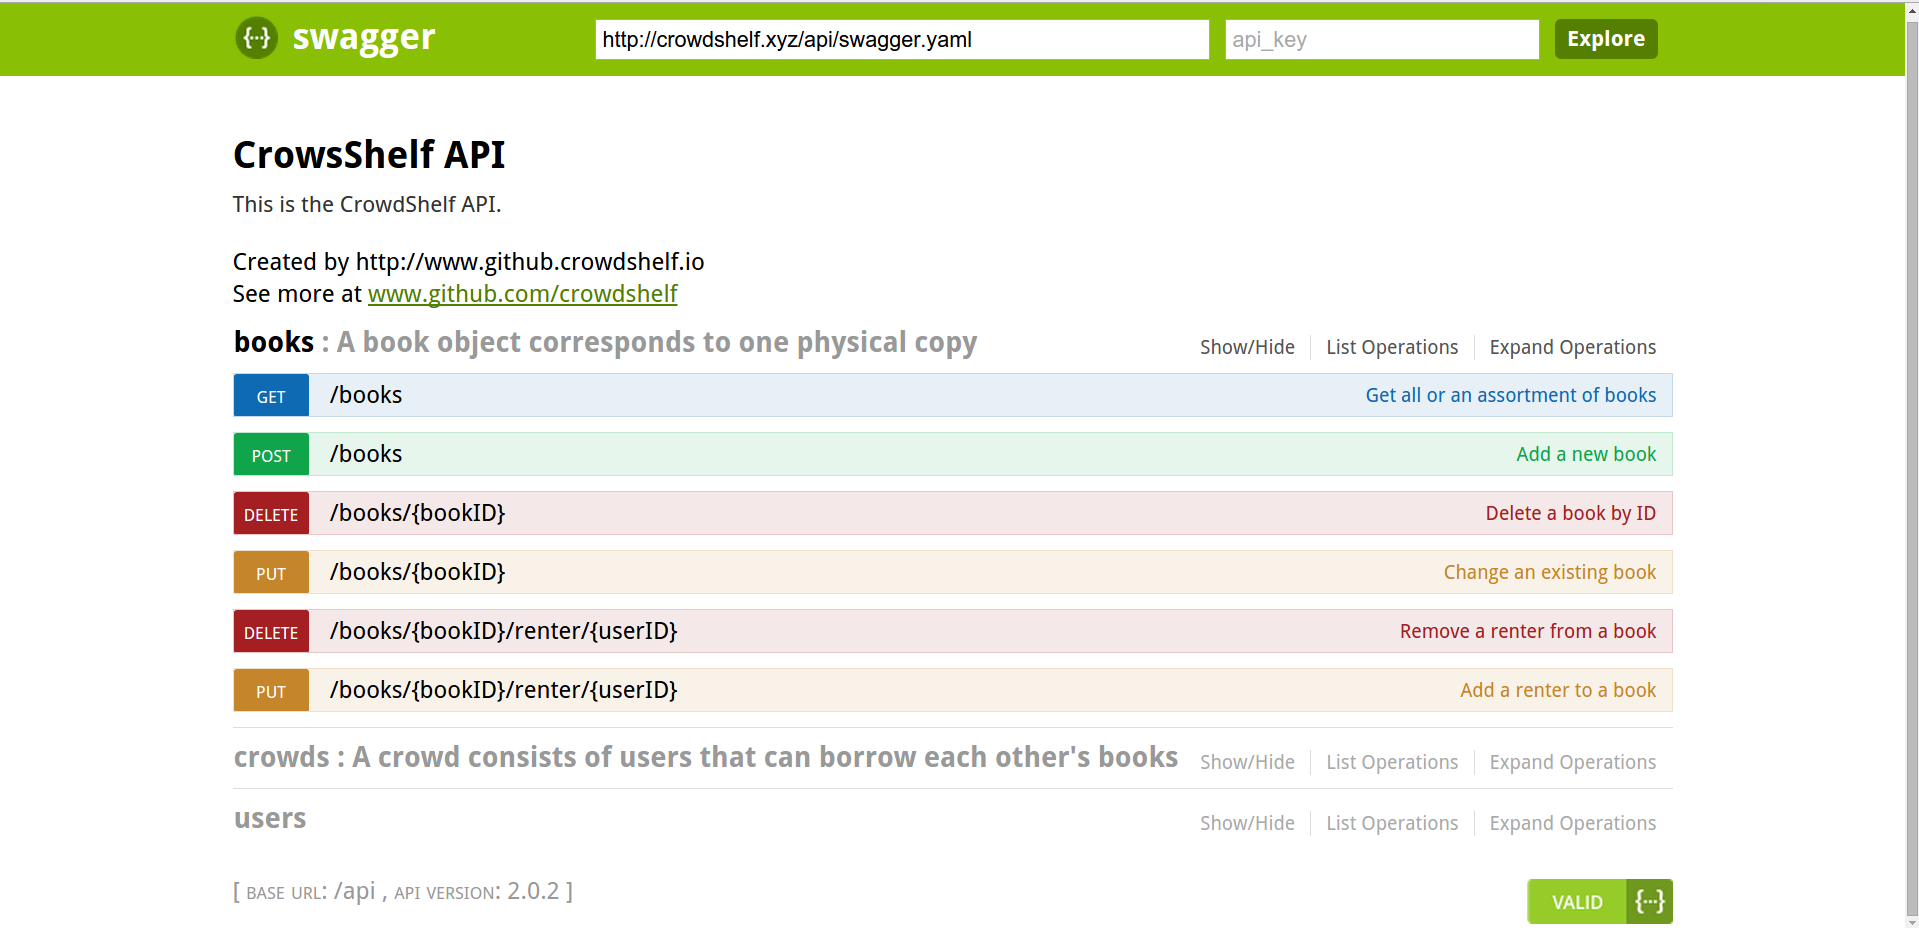
\includegraphics[width=\textwidth]{figs/v02/swagger2.png}
  \caption{Swagger with an overview of requests related to a specific entity.}
  \label{fig:swagger2}
\end{subfigure}%

\begin{subfigure}{\textwidth}
  \centering
  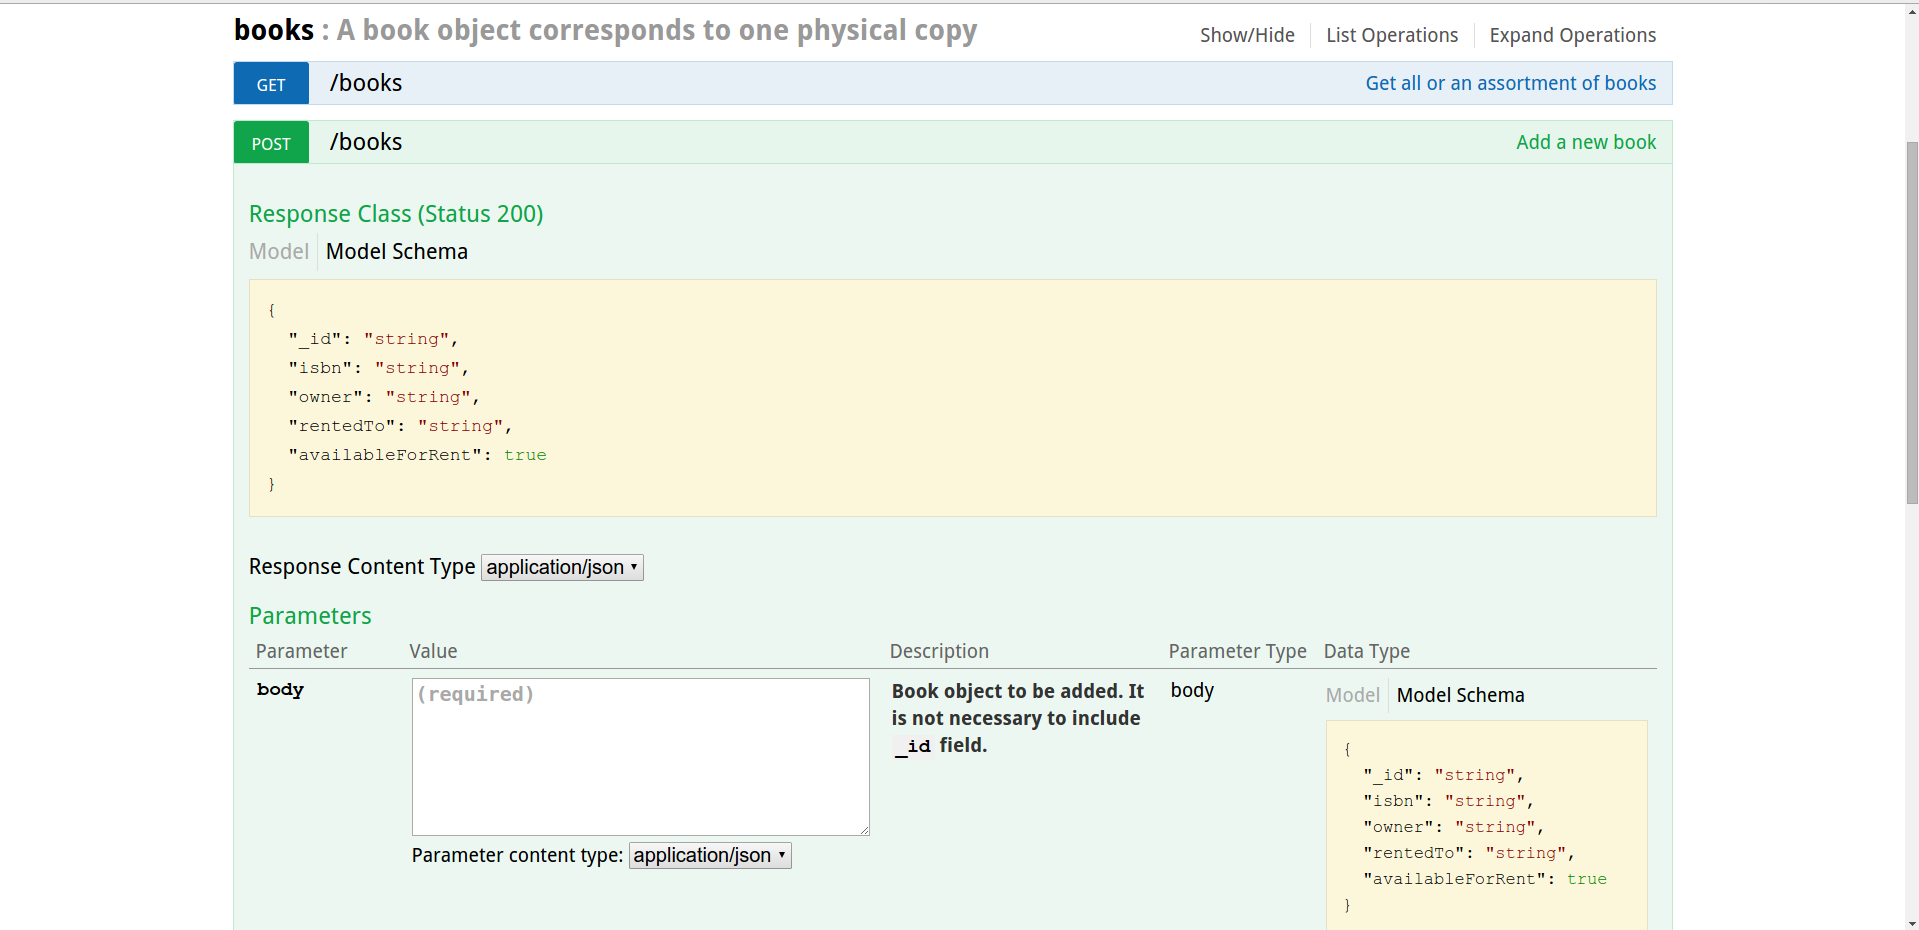
\includegraphics[width=\textwidth]{figs/v02/swagger3.png}
  \caption{Swagger when looking at a specific request.}
  \label{fig:swagger3}
\end{subfigure}
\caption{Screenshots from Swagger UI with the CrowdShelf \gls{API} specification}
\label{fig:02swagger-docs}
\end{figure}
\subsection{Feedback}

The feedback from the usability tests gave a positive indication that users would find it simple to add a book using a barcode scanner. Of the four users that were tested, three managed the tasks asked to complete without any trouble. The fourth subject had some trouble understanding the concept of the application, and as a consequence did not manage all the tasks without feeling very insecure in its use.

A few features of the application was mentioned to be improved. The users missed clear feedback when an action was taken, also the response was that the scanner button was easier to find if it was written scanner in contrast to an icon representing a camera. 

The finished version was sent to a few Netlight employees and students, but they were barely used. The customer representative was pleased with the increased velocity of the development, but this version was not yet ready to be used internally in Netlight. 

However, the team had received positive feedback regarding the features and usability of the application. Therefore it was decided to continue with the scanner solution and focus on the functionality chosen for the next version of the product. 

During this version a Facebook-page was also created to try to reach out to more users. The page gets updated every time a new version is released, and it contains a link to the project’s web page and to the Android application’s download page in Google Play. 

\subsection{Version progress}
As a consequence of the long duration of version 0.1, where no application was released, this version was completed very rapidly. In spite of a few obstacles, it took merely four days to complete four user stories with related 24 sub-tasks. As illustrated in figure \ref{fig:version-progress-2}, most tasks were completed on Monday and Wednesday when the whole team were working together. 

The release note found in appendix \ref{app:release-note-2} also show the consequence of a long first version iteration. Many of the tasks needed to complete the implementation of the applications were already completed before version 0.2.

The blog post used to describe the progress to the customer and supervisor are found in figure \ref{fig:week-five}.

\begin{figure}
\centering
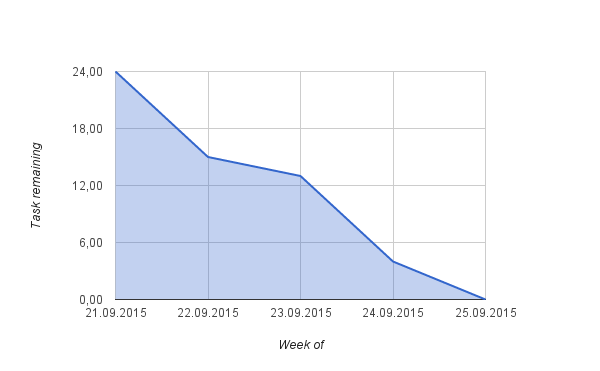
\includegraphics[height=10cm]{figs/v02/version-progress.png}
\caption{Task progression version 0.2}
\label{fig:version-progress-2}
\end{figure}

\begin{figure}
\centering
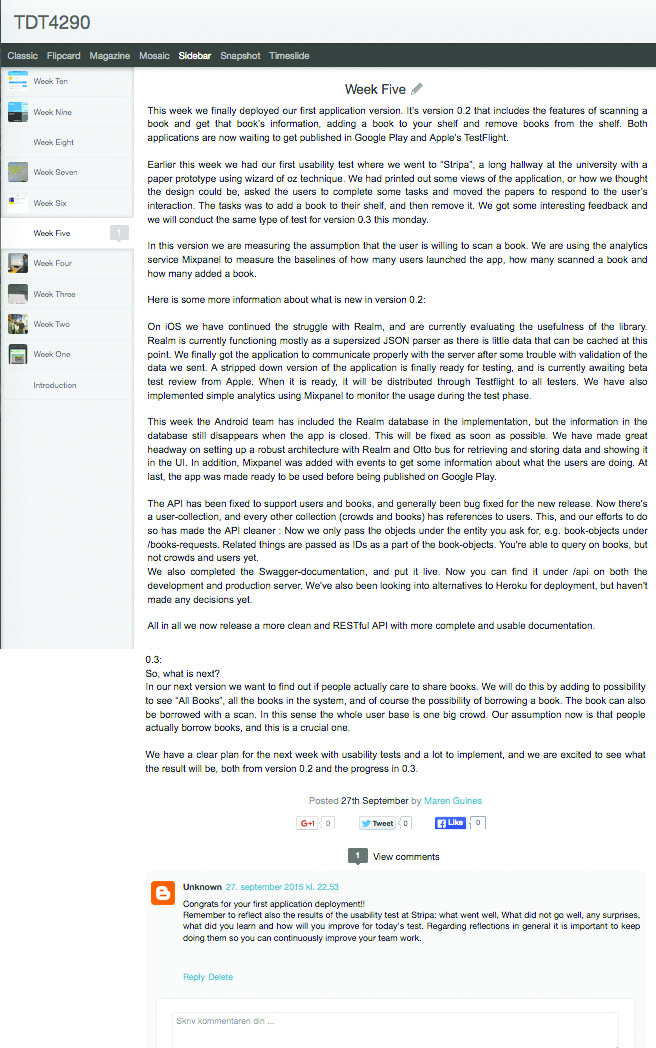
\includegraphics[height=22cm]{figs/v02/WeekFive.jpg}
\caption{Blog post from week 39}
\label{fig:week-five}
\end{figure}


\subsection{Review and retrospective}

At the customer meeting that was held during the second version, the team and the customer representative discussed the development progress. The customer representative stated that he missed the efforts he had seen the first weeks. The development had slowed down because of a lot of technical issues concerning the development of the Android application. Nevertheless, the team and the customer discussed possibilities to improve the progress. Increased use use of Netlight employees as support to the Android team would be an important factor in this effort. 

In addition, the customer representative had some input on what should be done before the next meeting. The design guidelines for iOS and Android should be studied, and a video of the application was to be shown at the next meeting.

One week later the customer representative was pleased with the development and the videos presented to show the functionality of the application. He always has a lot of feedback for the team to work on, and the team appreciates all his ideas and suggestions.

When the version was released, the team had a retrospective meeting where the overall atmosphere was positive. Communication within the team was mentioned under “What went well in this version”, as well as the fact that the application was released within the predetermined date. On the improvement side the team members mentioned the issue of having clear goals, and being able to work towards those goals. This will be the main focus point to try to improve in the next version.

Minutes from the costumer meeting is located in appendix \ref{app:customer-minutes-5}.

\subsection{Summary}
With the release of this version, it was possible to scan books to add and remove them from your virtual library, and browse all the books registered in the system.

Through usability tests an initial indication on the validity of the versions assumption was received, and a design of the functionality of the application version 0.2 was created.

The applications were completed on time and distributed through Google Play and TestFlight. Unfortunately the app was not downloaded enough to get any useful data from users this version either. The customer representative, who represent a lot of users in Netlight, seemed pleased with the results of the iteration.


% Version 0.3
\section{Version 0.3}

In the third version the goal was to learn if people actually want to use the application to keep track of books they borrow or have lent to others. From the previous versions the indication says that they do, but according to Lean Startup it is not possible to know if it is correct until it can be proven scientifically with data measured. As in the earlier versions this version contains two iteration, one for with paper prototypes and one with the implemented application.
\subsection{Assumption and questions}
The assumption to be confirmed for this iteration was
“Users want to borrow books and be able to keep track of who has borrowed the book and who they have borrowed the book from”.

Questions needed to confirm this assumption: 
\begin{enumerate}
\item Is there a market for borrowing books among the users?
\item Do the users tend to have trouble remembering who they borrowed a book from?
\item Is it a problem for the users to remember what books are borrowed?
\end{enumerate}

\subsection{Planning and design}
To confirm the assumption selected in this version, the team had to learn about the users book habits. How often the users borrow books and how often there is a problem keeping track of a book, are essential issues to learn how the users will adapt to the application. In obtaining these answers, the team planned to do a usability test with questions for the students and to ask the employees at Netlight. 

Indeed the most vital information about the users is collected by measuring the use of the application, but because of the application’s small user base those numbers may also be an unrepresentative result. One of the reasons the application has not managed to get the desired number of users is that the application is not satisfying to be a product, or minimal viable product to Netlight. Because of this the customer representative will deploy the application to Netlight when certain functionality is implemented and until then the team should follow the \gls{LSU} with numbers from prototypes and surveys, and of course the small amount of data retrieved from users of the application. 

In developing a paper prototype the team discussed the different possibilities of how to represent the borrowed and lent books, in addition to the representation of a borrow-functionality. The different possibilities were drawn on the whiteboard in accordance to Lean UX and eventually the team agreed upon a design. Because of the new feature of showing what books a users has lent, the shelf view was switched from alternative 1 to alternative 2 shown in figure \ref{fig:design-alternatives-v2}, but with three lists instead of two. The new paper prototype created is illustrated in figure \ref{fig:prototype-v3} where each view was a cut out in phone size when presented to the users. 

From the discussion of functionality needed in this version to learn about the assumption, five user stories were selected as requirements. These are shown in \ref{user-stories-v3}. When conducting the usability test these stories were used as basis for the tasks the participants had to complete. 

\begin{figure}
\centering
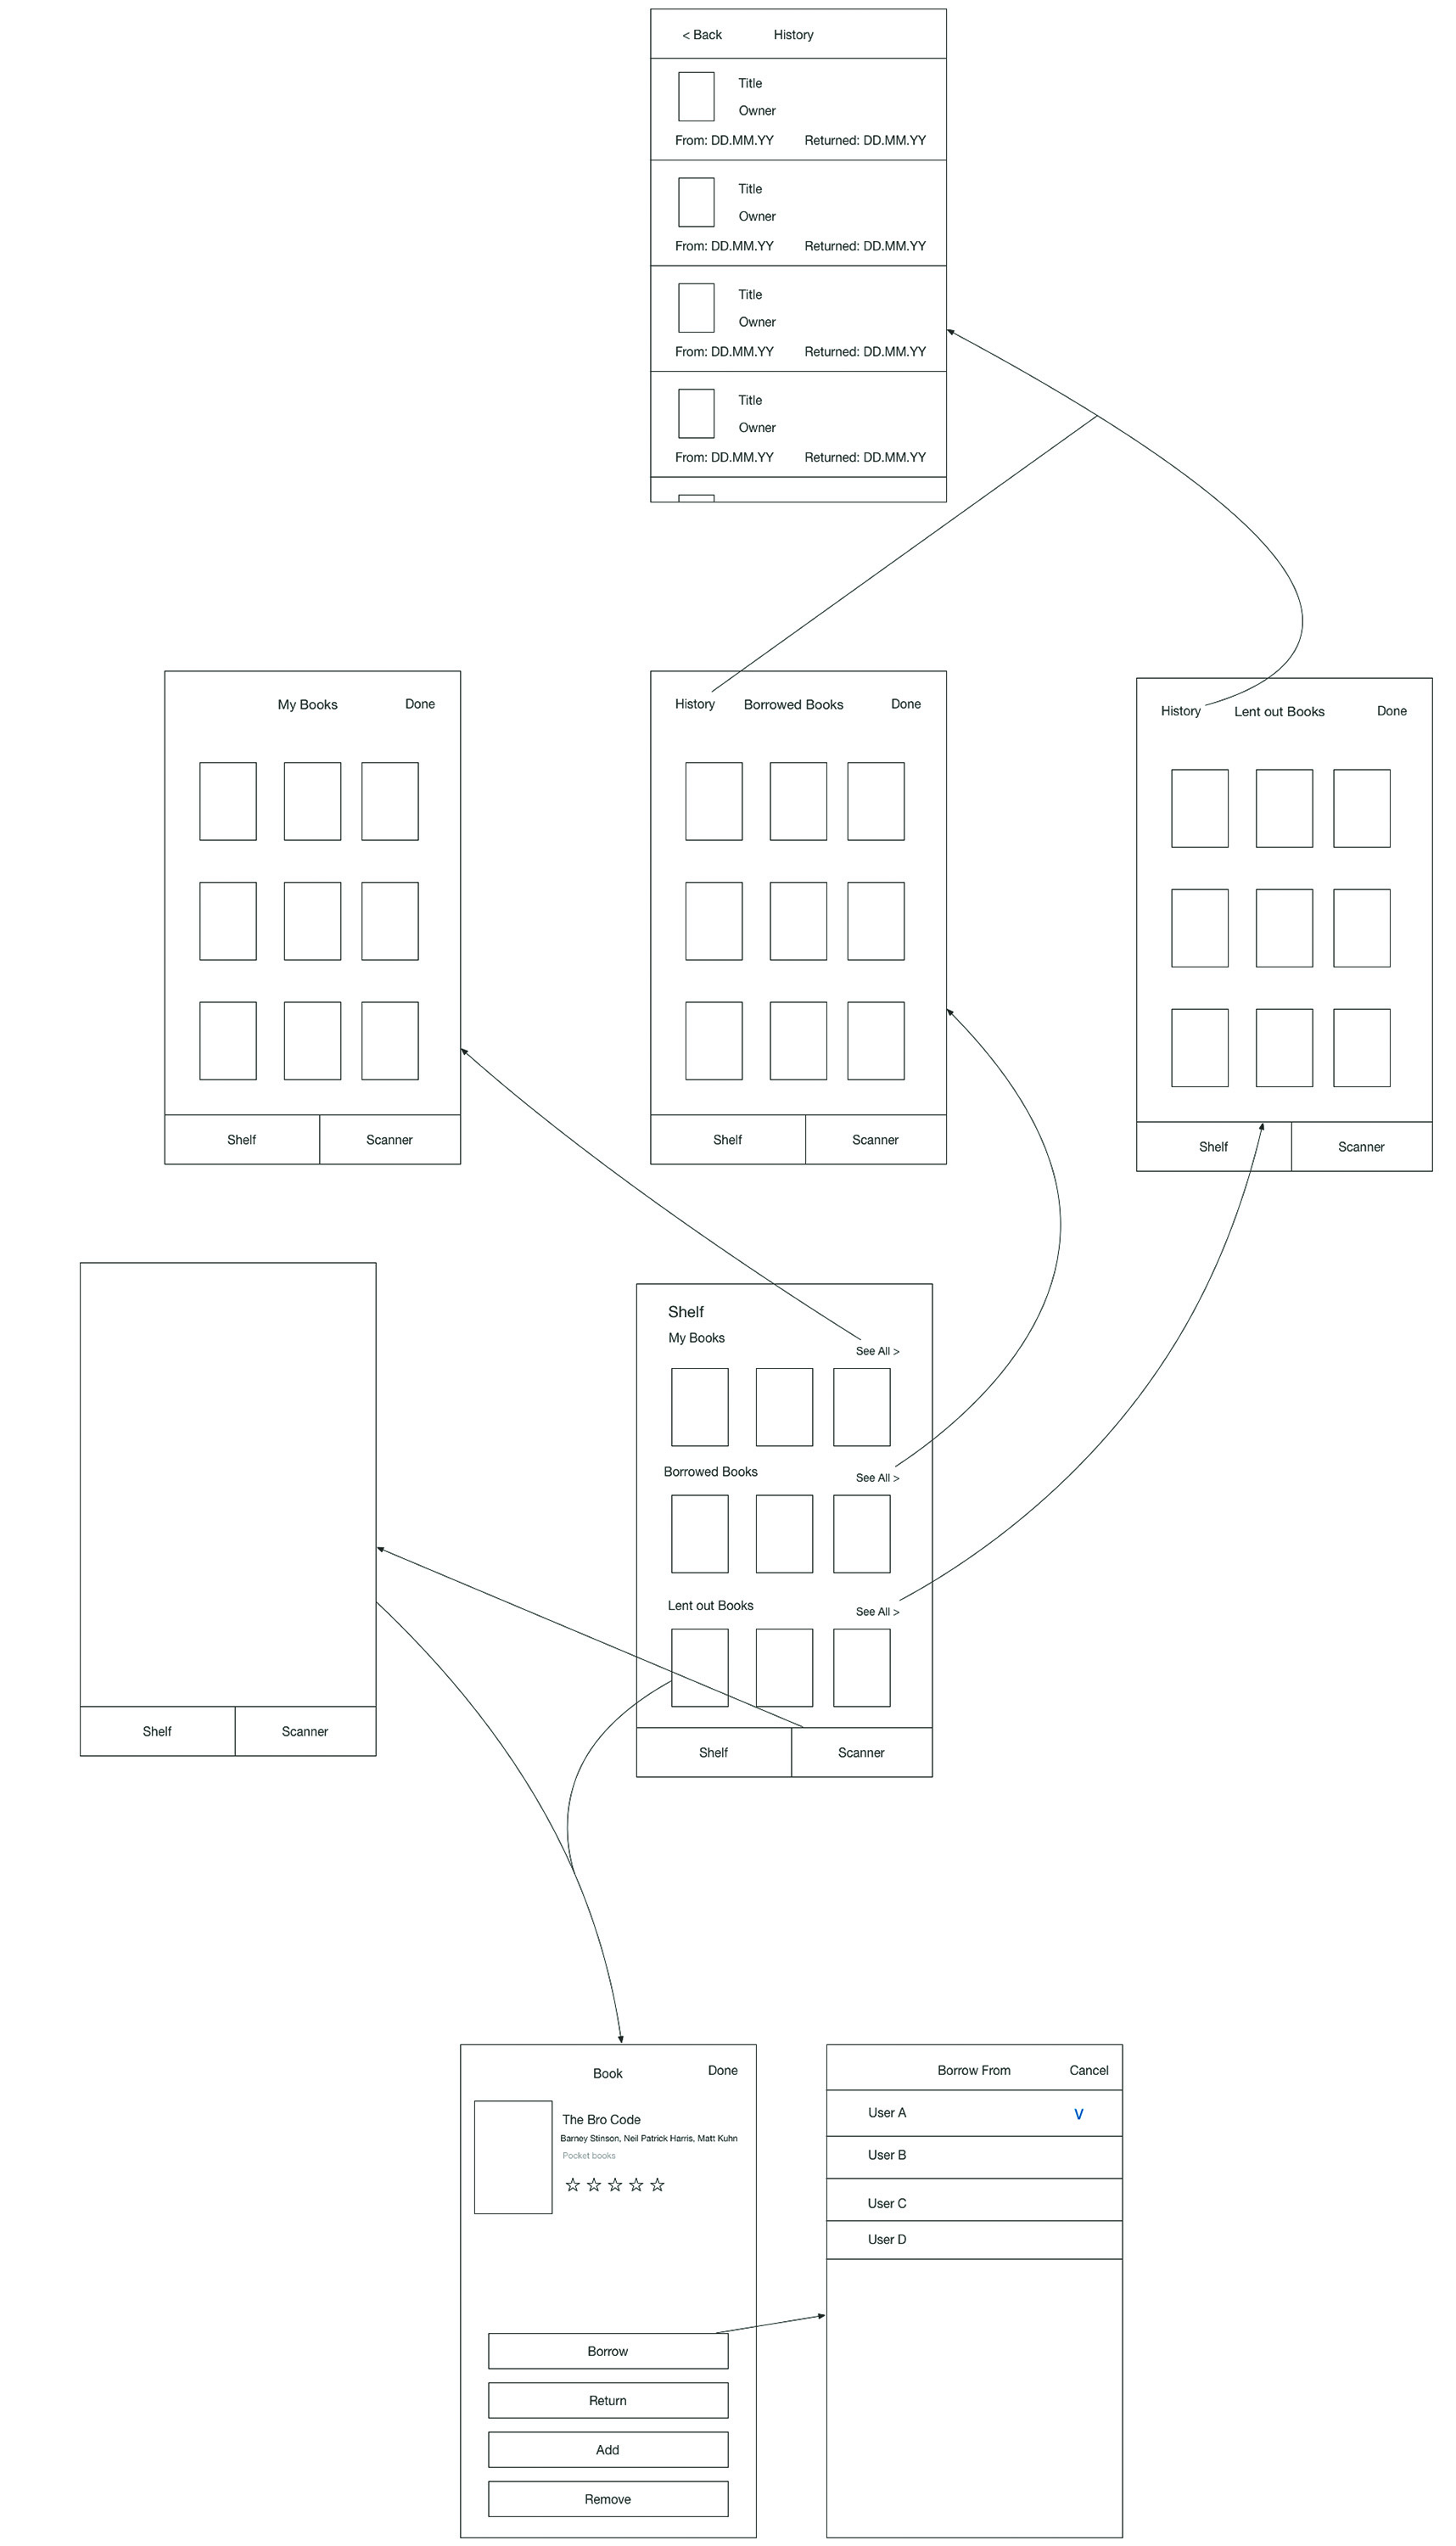
\includegraphics[height=20cm]{figs/v03/prototypesv3.jpg}
\caption{Relationship between views of paper prototype for CrowdShelf version 0.3}

\label{fig:prototype-v3}
\end{figure}

The usability test started with explaining the product, then the users were given the start screen and asked to complete the following tasks:
\begin{enumerate}
\item Borrow a book.
\item See a list of all books you own, but are lent out.
\item See a list of all books you have that are not yours.
\item Return a book you have borrowed.
\end{enumerate}

After the test was completed the application had a design of the functionality and the team was ready to implement the user stories in the application.




\subsection{User stories}
\label{user-stories-v3}
This section shows the user stories selected as requirements version 0.3. The stories are selected based on the assumption thought to be the most relevant to test the features of the product. 

\begin{enumerate}
  \item As a user I want to borrow a book from another member  
  \item As a user I want to return a book that i have borrowed
  \item As a user I want to see the owner and holder of all copies of a book
  \item As a user I want to see a list of all the books I'm currently borrowing
  \item As a user I want to see a list of all the books I'm lending to others
\end{enumerate}



\subsection{Development}
Developing the new features of this version was easier than the earlier version because the development teams were starting to get a better take on the implementation. This section explains in detail what was created during this version iteration in the three different sub teams.

\subsubsection{Android}
\begin{description}
    \item[Features] \hfill\\
The first task the Android team focused on for this version was the ability to borrow a book from another user, and register this for both users involved. To be able to do this, the application needed to show which users who owned a specific book, and then be able to select a user to borrow this book from. To implement this a group were created containing all the Android users of the application. This was done because the team had future releases in mind, which probably would include the possibility to create groups of users. Therefore instead of implementing the possibility of listing all users, which would not be used later at any time, the team implemented a solution were all users where in a single group, and then listing the members of this group, a feature that was probably going to get used in future releases. 

Then, when a user wanted to borrow a book, the group was filtered on who owned this book, and a list of relevant users was shown in the application. If the user then chose another user to borrow the book from a request would be sent to update the \gls{backend} with the new information containing a new renter of this book. This borrowed book would then appear in the user's book shelf. The borrower could also, in this version, return the book by viewing its book information and clicking the return button. 

Simultaneously while implementing the features above, the ability to create a user and login with a specific username was implemented. This version supported creating of a user containing username, name and email. Since password authentication was not yet implemented on the \gls{backend}, this was also excluded from the Android application for this version. This feature allowed the user to interact with other users both on Android and iOS, making it finally usable to some extent. 

    \item[Structure] \hfill\\
As seen in figure \ref{fig:AndroidStructure03} this version added two more activities, \code{LoginActivity} and \code{UserListActivity}. The \code{MainTabbedAcitivty} activity is still the main activity, meaning the activity that is initially started when the application launches. Instead of immediately showing the users books, the \code{MainTabbedActivity} activity now starts a \code{LoginActivity} activity to force the user to sign in with an existing user or create a new one. The new \code{UserListActivity} activity was also added to support the feature to borrow a book from another user. This activity shows a list of users that owns a specific book, and is started from the \code{ViewBookActivity} activity. 

\begin{figure}
\centering
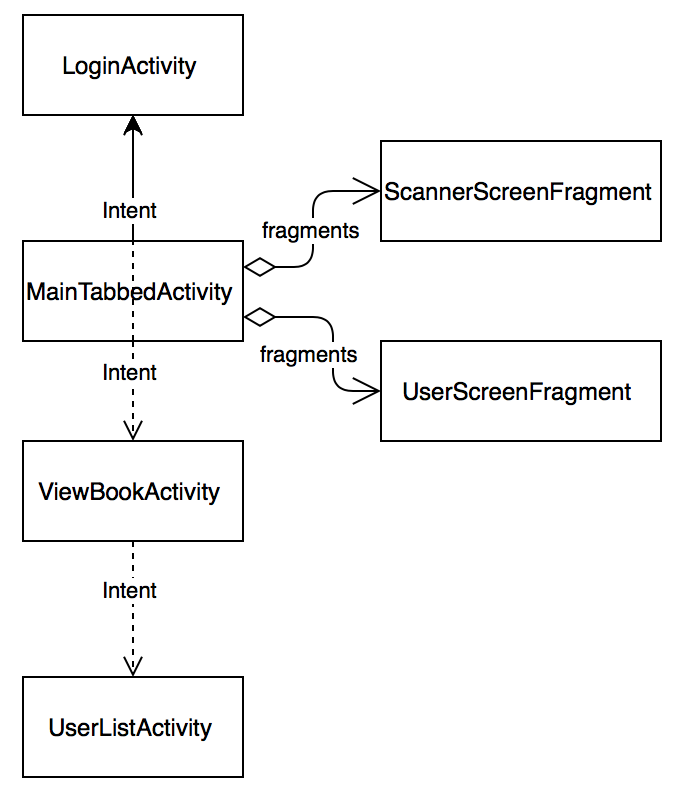
\includegraphics[height=7cm]{figs/v03/AndroidStructure-03.png}
\caption{Basic Android version 0.3 structure}
\label{fig:AndroidStructure03}
\end{figure}

    \item[Design] \hfill\\
There was not done any big changes with the design for this version, but most of the buttons, images and text were made bigger to follow the design standards. How it looked when the owner of a book looked at its information in version 0.3, is shown in Figure \ref{fig:book-view-v3}. More feedback of user actions was also added in this version, for instance showing a loading spinner when book information is loading.  

\begin{figure}
\centering
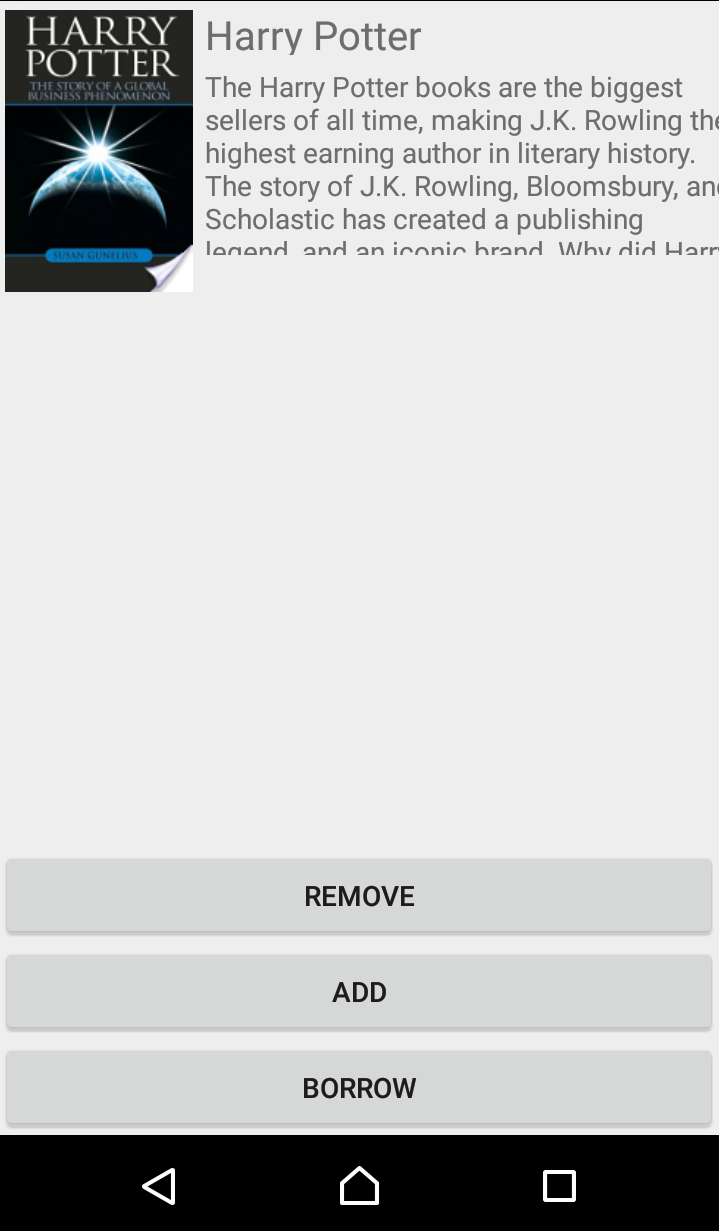
\includegraphics[height=7cm]{figs/v03/bookView03.png}
\caption{The activity showing book information in version 0.3 of the application}
\label{fig:book-view-v3}
\end{figure}

    \item[User feedback] \hfill\\
To get feedback on the new implemented features, more events where added to Mixpanel. Mixpanel now also allowed the application to track when a book was borrowed and when a book was returned. See table \ref{tab:mixpanel_table}.

    \item[Bug fixes] \hfill\\
After the version 0.2 of the application had been used, some errors were discovered. For instance, if a user scanned a barcode that could not be found in Google Books, the application crashed and displayed an error message. This was solved by handling the error from Google Books and displaying a message to the user that the book was not found. Another bug discovered in the last version was that the applications local realm database was deleted when the application closed, which meant that next time the application was launched the information stored in the database was no longer available. 
\end{description}

\subsubsection{iOS}
\begin{description}
    \item[Features] \hfill\\
The goal for this version for the iOS team was to make it possible to borrow books from other users, and return them. In order to borrow a book, the user had to scan the barcode, press the borrow button, and select the owner of the book form a list. As there were no way to filter owners at this point, all users who had the given book in their shelf would be displayed. When an owner was selected, a request would be sent to the \gls{backend} to update the information in the database.

Because borrowing books raised the need to identify individual users, a login feature had to be implemented. This was done by creating a new login view, and setting the user model representing the currently authenticated user as a class variable on the \code{User} class. Therefore, the local user would be accessible from all parts of the application. Which was beneficial when retrieving books, crowds and users related to the local user, from the server.

    \item[Design] \hfill\\
The overall design from version 0.2 was extended to include the new buttons necessary to borrow and return books. Some additional feedback was added to provide the user some information about the state of the application.

    \item[User feedback] \hfill\\
The integration of Mixpanel from version 0.2 was extended to also include reporting borrow and return events for books. This would allow the team to monitor how the new features were used.
\end{description}

\subsubsection{Backend}
The \gls{backend} seems mostly finished for books and book loans after the release of version 0.2, so the team just focused on bug fixes for those two areas. This means that there have not been that much real implementation for the \gls{backend} team this iteration. The team implemented a lot of \gls{ID}-validation, for instance that a user \gls{ID} that is added to a book as a loaner, actually is a user in the database.

For this version the \gls{backend} team researched APIs for getting information on norwegian books. The team also did a lot of research on the Docker software container framework, as the customer wanted us to wrap the whole \gls{backend} solution in it. \cite{docker} The team also looked more into deployment platforms, as the limitations of the free version of Heroku had become apparent. At this point the team were using the free level of service they offer, which is not much. \cite{heroku-pricing} It does not offer 24/7 uptime, which the team want for the server serving the stable API. The free level has to sleep 6 hours of every 24 hours. This means the service will be unreachable for a fourth of every 24 hours. 

To meet the demands the team looked after other options. The team talked to Microsoft about their Dreamspark-licenses (license for students) and what it gives access to on Microsoft Azure. \cite{microsoft-dreamspark} After talking with Microsoft on the phone, the team found that the DreamSpark-license does not cover running a server written in Node.

In addition the domain \url{http://crowdshelf.xyz} was bought, and \gls{PaaS}s like Digital Ocean was researched.\cite{digitalocean} The team decided to rent a so called ''droplet'', a virtual machine, from Digital Ocean. The domain was pointed at that virtual machine. Also see the preliminary studies, section \ref{prelim-digitalocean}, for more research on this \gls{PaaS}.


\subsection{Feedback}
From the feedback shown in table \ref{feedback-3} the team continued with the layout selected in the paper prototypes with focus on implementing clear feedback to the users when taking an action. 
\begin{table}[]
\centering
\begin{tabular}{|L{1.5cm}|L{1cm}|L{3cm}|L{7cm}|}
\hline
\textbf{Gender} & \textbf{Age} & \textbf{Occupation} & \textbf{Problems/ comments} \\
\hline
Male & 20-30 & Student & Completed all the tasks without ant problemts. Would like to confirm when returning a book. \\
\hline
Female & 20-30 & Student & Completed the tasks, but did not find the “done”-button immediately. Would also like an explanation of the buttons first time the app is used. \\
\hline
Male & 20-30 & Student & Completed the tasks without difficulty, but would like an explanation of the buttons in Viewbook, specially remove vs return. \\
\hline
Female & 20-30 & Student & Did not understand the scanner, and had difficulties with the concept of the application. \\
\hline
\end{tabular}
\caption{Feedback regarding the usability test of the paper prototype of version 0.3}
\label{feedback-3}
\end{table}
Regarding feedback from the use of the application the team has obtained some new users, but still not enough to make the numbers applicable for analysis to learn from. 

Although there still is a question of how many users can be obtained to collect user data from the application, the analysis done from questions and usability test gave some answers to the assumption of this version. The answer to the question about whether the users are borrowing books is twofold. The same is the case for the answer about if they are having trouble keeping track of where those books are.

At this stage the applications main user base is students and companies, and the book habits are quite different in those two areas. The students tend to borrow books about twice a year (each semester), while the employees at Netlight often borrow books from the company. In both cases people have some trouble keeping track of the books, but this problem is somewhat more relevant amongst the students. 

As a result of these results the team decided to focus on the company needs of the application. The students are still welcome to use the application, but because they borrow books so rarely there will not be enough use of the application to get some real data from their use. 


\subsection{Version progress}

In this version the progression has continued in a stable manner with tasks being completed within their due date. At the end of the version, as shown in figure \ref{fig:progress-3}, four of the team members had a big delivery in another course, so the progress want a little slow those days. However in an overall manner the progression of the project has stabilized, much because the team members have achieved a deeper understanding of the technologies they are working with, and also the concepts and ideas behind the Lean Startup.

Observed in appendix \ref{app:release-note-3}, the release note of version 0.3, almost all the tasks completed are related to the user stories selected for the version. This is due to the focus of the version of having clear goals and trying to do what has to be done to complete the version instead of fixing other problems. Of course there are tasks that has to be completed not related to the stories, but the team worked towards a common goal that they all felt they had decided together. 

The blog posts to keep information flow to the customer and supervisor are shown in figure \ref{fig:week-six} and \ref{fig:week-seven}. These explain what is performed by the team the weeks of the iteration that is version 0.3, both technical and non-technical.



\begin{figure}
\centering
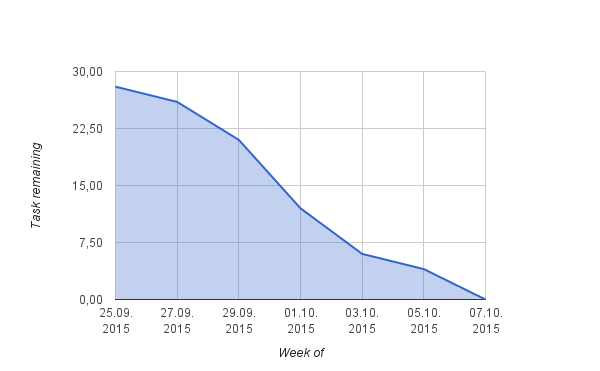
\includegraphics[height=10cm]{figs/v03/progress3.png}
\caption{Task progress version 0.3}
\label{fig:progress-3}
\end{figure}

\begin{figure}
\centering
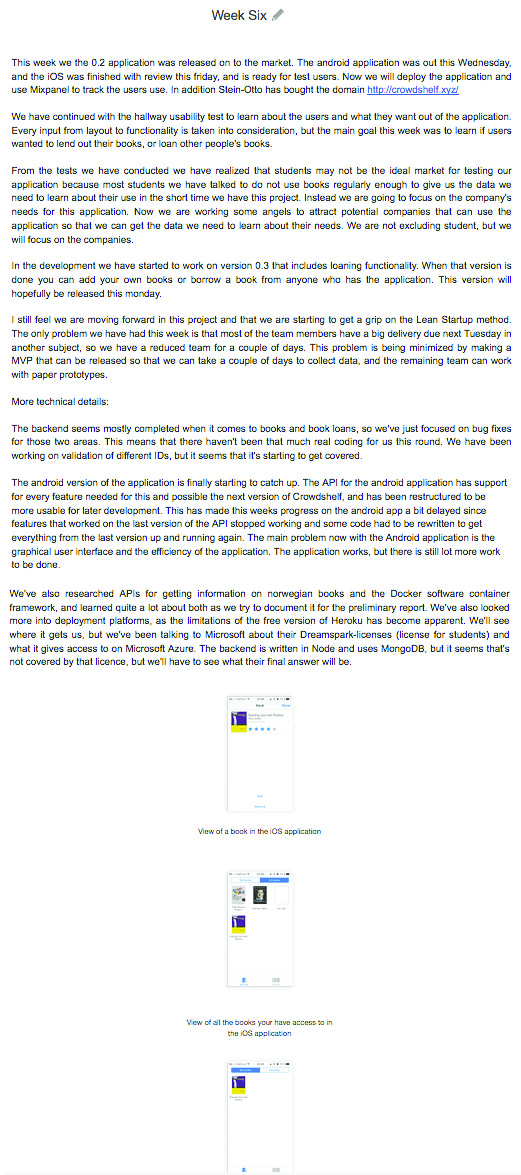
\includegraphics[height=22cm]{figs/v03/WeekSix.jpg}
\caption{Blog post from week 40}
\label{fig:week-six}
\end{figure}

\begin{figure}
\centering
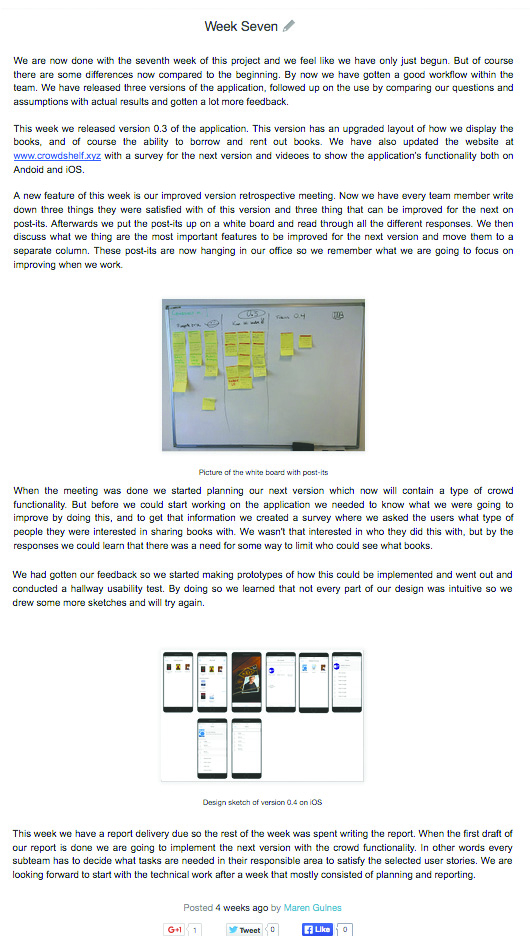
\includegraphics[height=22cm]{figs/v03/WeekSeven.jpg}
\caption{Blog post from week 41}
\label{fig:week-seven}
\end{figure}

\subsection{Review and retrospective}
During this version the team decided, together with the customer representative, to focus on the company parts of the application, and to satisfy those needs. In discussion with him the team came up with some potential businesses that had mentioned their interest in the application. The interests were a primary school in Oslo and the police attorneys at Grønland police station.

Minutes from the costumer meeting is located in appendix \ref{app:customer-minutes-6} and \ref{app:customer-minutes-7}.

As a consequence of the possible new interests a new feature was discussed, namely the development a custom book information provider. The teams \gls{backend} lead research to see if he could find any norwegian book information provider that could satisfy the need to those potential new businesses, but ended up concluding there was no such API. With that as basis the idea of a new system to support this came to life. 

When version 0.3 of the application was released the team had a retrospective meeting. As of this version that meeting was performed in a different manner than the previous retrospective meetings. From a suggestion from the customer representative, the meeting was now performed using post-it notes and whiteboard. Every team member wrote down three things they thought went well during the version, and three points they thought could be improved. Out of those points, two were selected to be the main focus in the next version. 

As illustrated in the picture of the whiteboard found in figure \ref{fig:retrospective-3} the “Went well” column and “Can be improved” have approximately the same amount of notes. A goal of the project is to shorten down the “Can be improved column”. The positive aspects of this version are focused around the improvements in development and the communication within the team, and between sub-teams. The improvement points were mainly about getting a better structure within the Android team, and to continue to work on upholding the version control and JIRA delegation. 

The focus points from version 0.3 were the delegation of tasks within the Android team, and improving the connection between the iteration results and the assumption selected in the version. To improve the task delegation in the Android team, the Android lead should focus on creating tasks to the selected user stories and delegate them to the other team members. To improve the coupling between assumption and results the assumption will be written down for each iteration, and each result will be measured with thought to the assumption.

\begin{figure}
\centering
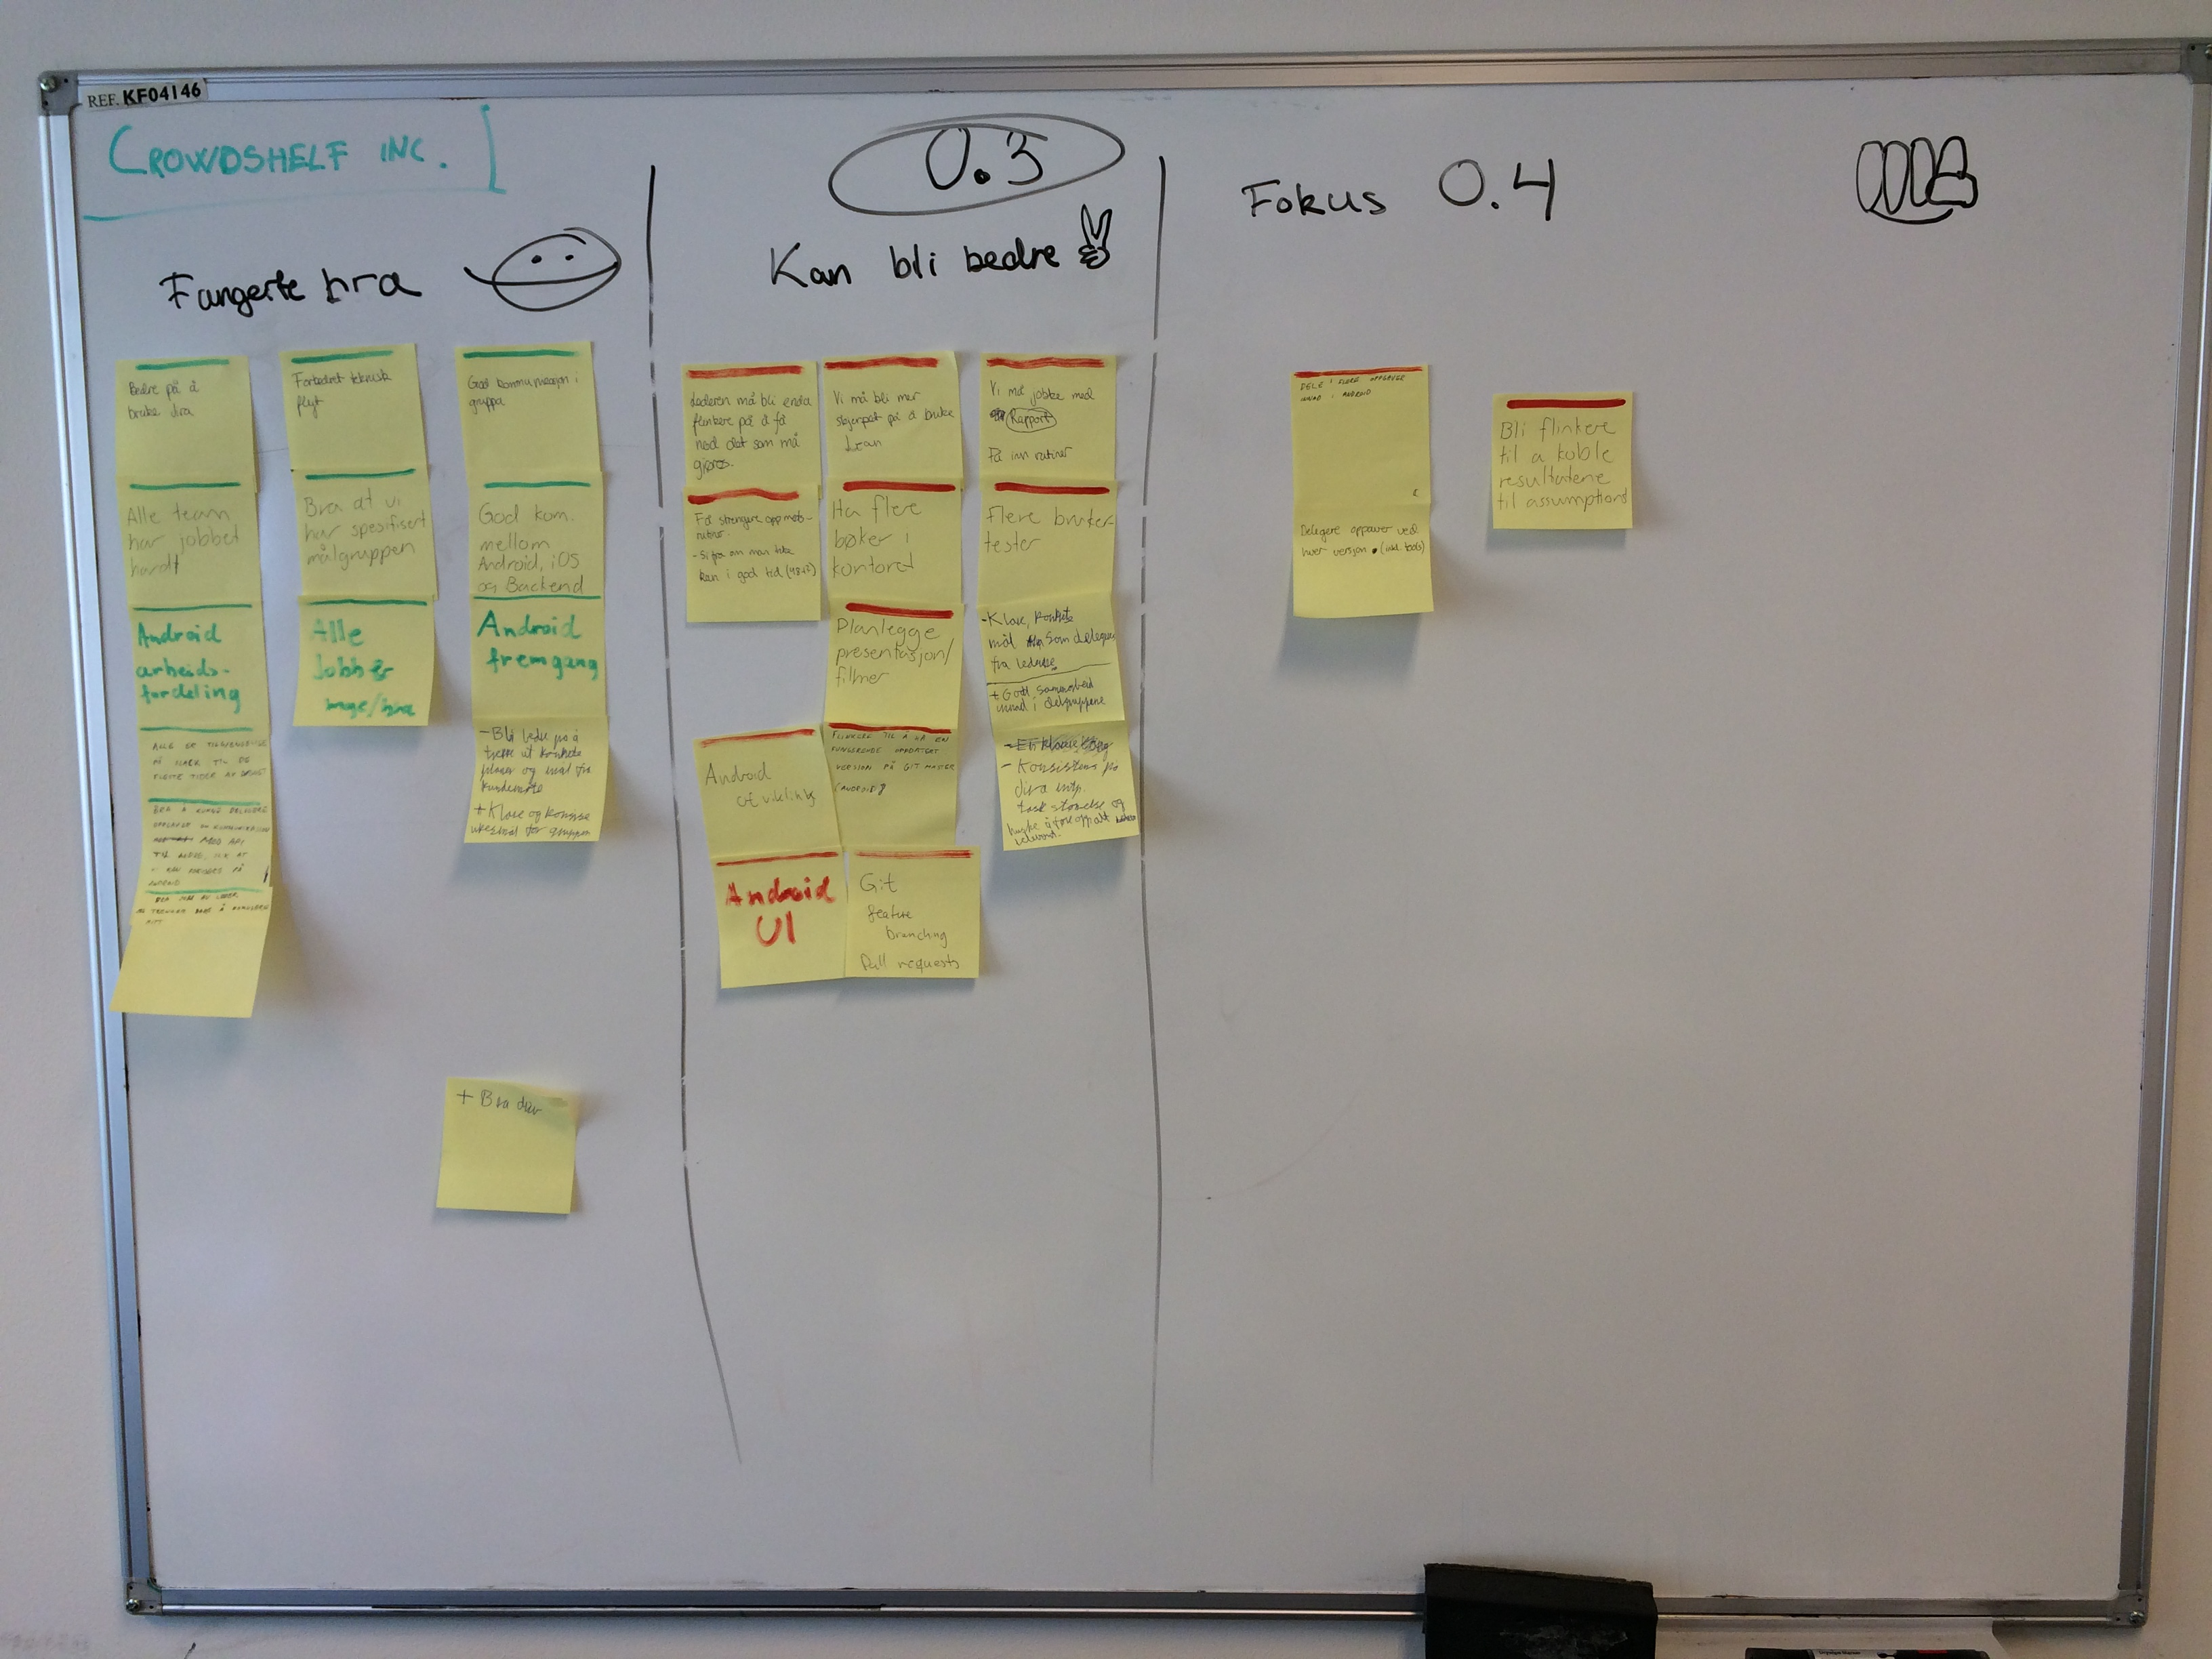
\includegraphics[height=10cm]{figs/v03/retrospective-3.JPG}
\caption{Picture of the whiteboard from retrospective meeting of version 0.3}
\label{fig:retrospective-3}
\end{figure}

\subsection{Summary}
At the beginning of version 0.3 the assumption was that the users borrow books and from time to time have trouble keeping track of where those books are in the sense of who the user have borrowed the book from or to. What was learned during this version was that the student users do not borrow book often enough to be a priority user in this project. Businesses on the other hand have a lot of books that people can borrow on a daily basis. 

As a consequence of the results the team has decided in agreement with the customer to focus on the business needs in the application. One of those needs is a possible book service where the users can add their own books if it does not exist in the Google Books database. The team will also focus on learning about the real business needs in association with the application in the next version by sending out a survey asking about their book habits. Until now their book habits are only gotten by asking unofficially and are therefore only indications.

The change in the performance of the retrospective meeting made it easier to get all the team members opinions and gave the team a constant visual, as the notes always were up on the board of what they had agreed to focus on.   


\clearpage
\section{Version 0.4}
The goal of this iteration and version was to implement the possibility to limit access to a users books. This was done by creating an assumption with questions to be answered, select the the user stories needed to support that feature and measure the use.

\subsection{Assumption and questions}
The assumption for this version was "Users only want to share books with a selection of other users"

In order to confirm this assumption, the team created a set of questions to be answered:

\begin{enumerate}

  \item Do users want to exclude users from borrowing their books?
  \item Do users want to to know the people they share books with?
  \item Do users need a crowd to share a book?
  \item Are users interested in organizing their network in a crowd form?
  \item Is security more important than efficiency?
  \item Do users want the ability share books with users that do not have the application?
  \item Do users want to share all their books with all users in their crowds, or be able to customize which books are available in a certain crowd?
  \item Are users more interested in which books are in a crowd, or the members?
\end{enumerate}


\subsection{Planning and design}

Based on the assumption, the team had to select a set of user stories needed to allow users to limit the access to their books. These user stories would be implemented in the mobile applications and the \gls{backend}. This would allow the team to measure the usage of the application in order to get and indication of whether the users wanted the crowd feature, or not.

A survey trying to answer the questions was created in order to get feedback from potential users. The feedback was used to discover what level of security and restrictions users wanted for their books. The survey was added to the website, linked on Facebook, and distributed to the \gls{IDI} at \gls{NTNU}.

Design sketches were made based on the features to be implemented, internal discussions, and feedback from Netlight employees. These sketches were used in \gls{guerrilla test} at the university. After having conducted usability tests with students in all previous versions, it was apparent that students had little trouble using the application, and the team realised that they were not necessarily representative users. Therefore it was decided to find test users who were less used to mobile platforms. The usability tests were performed with employees at \gls{IDI}, and the results were noticeably different. The users spent more time trying to figure out how to navigate the application, and one user did not manage to complete the tasks given. The design was revised, and new tests were conducted. The test users found the new design more intuitive.

\begin{figure}
    \centering
    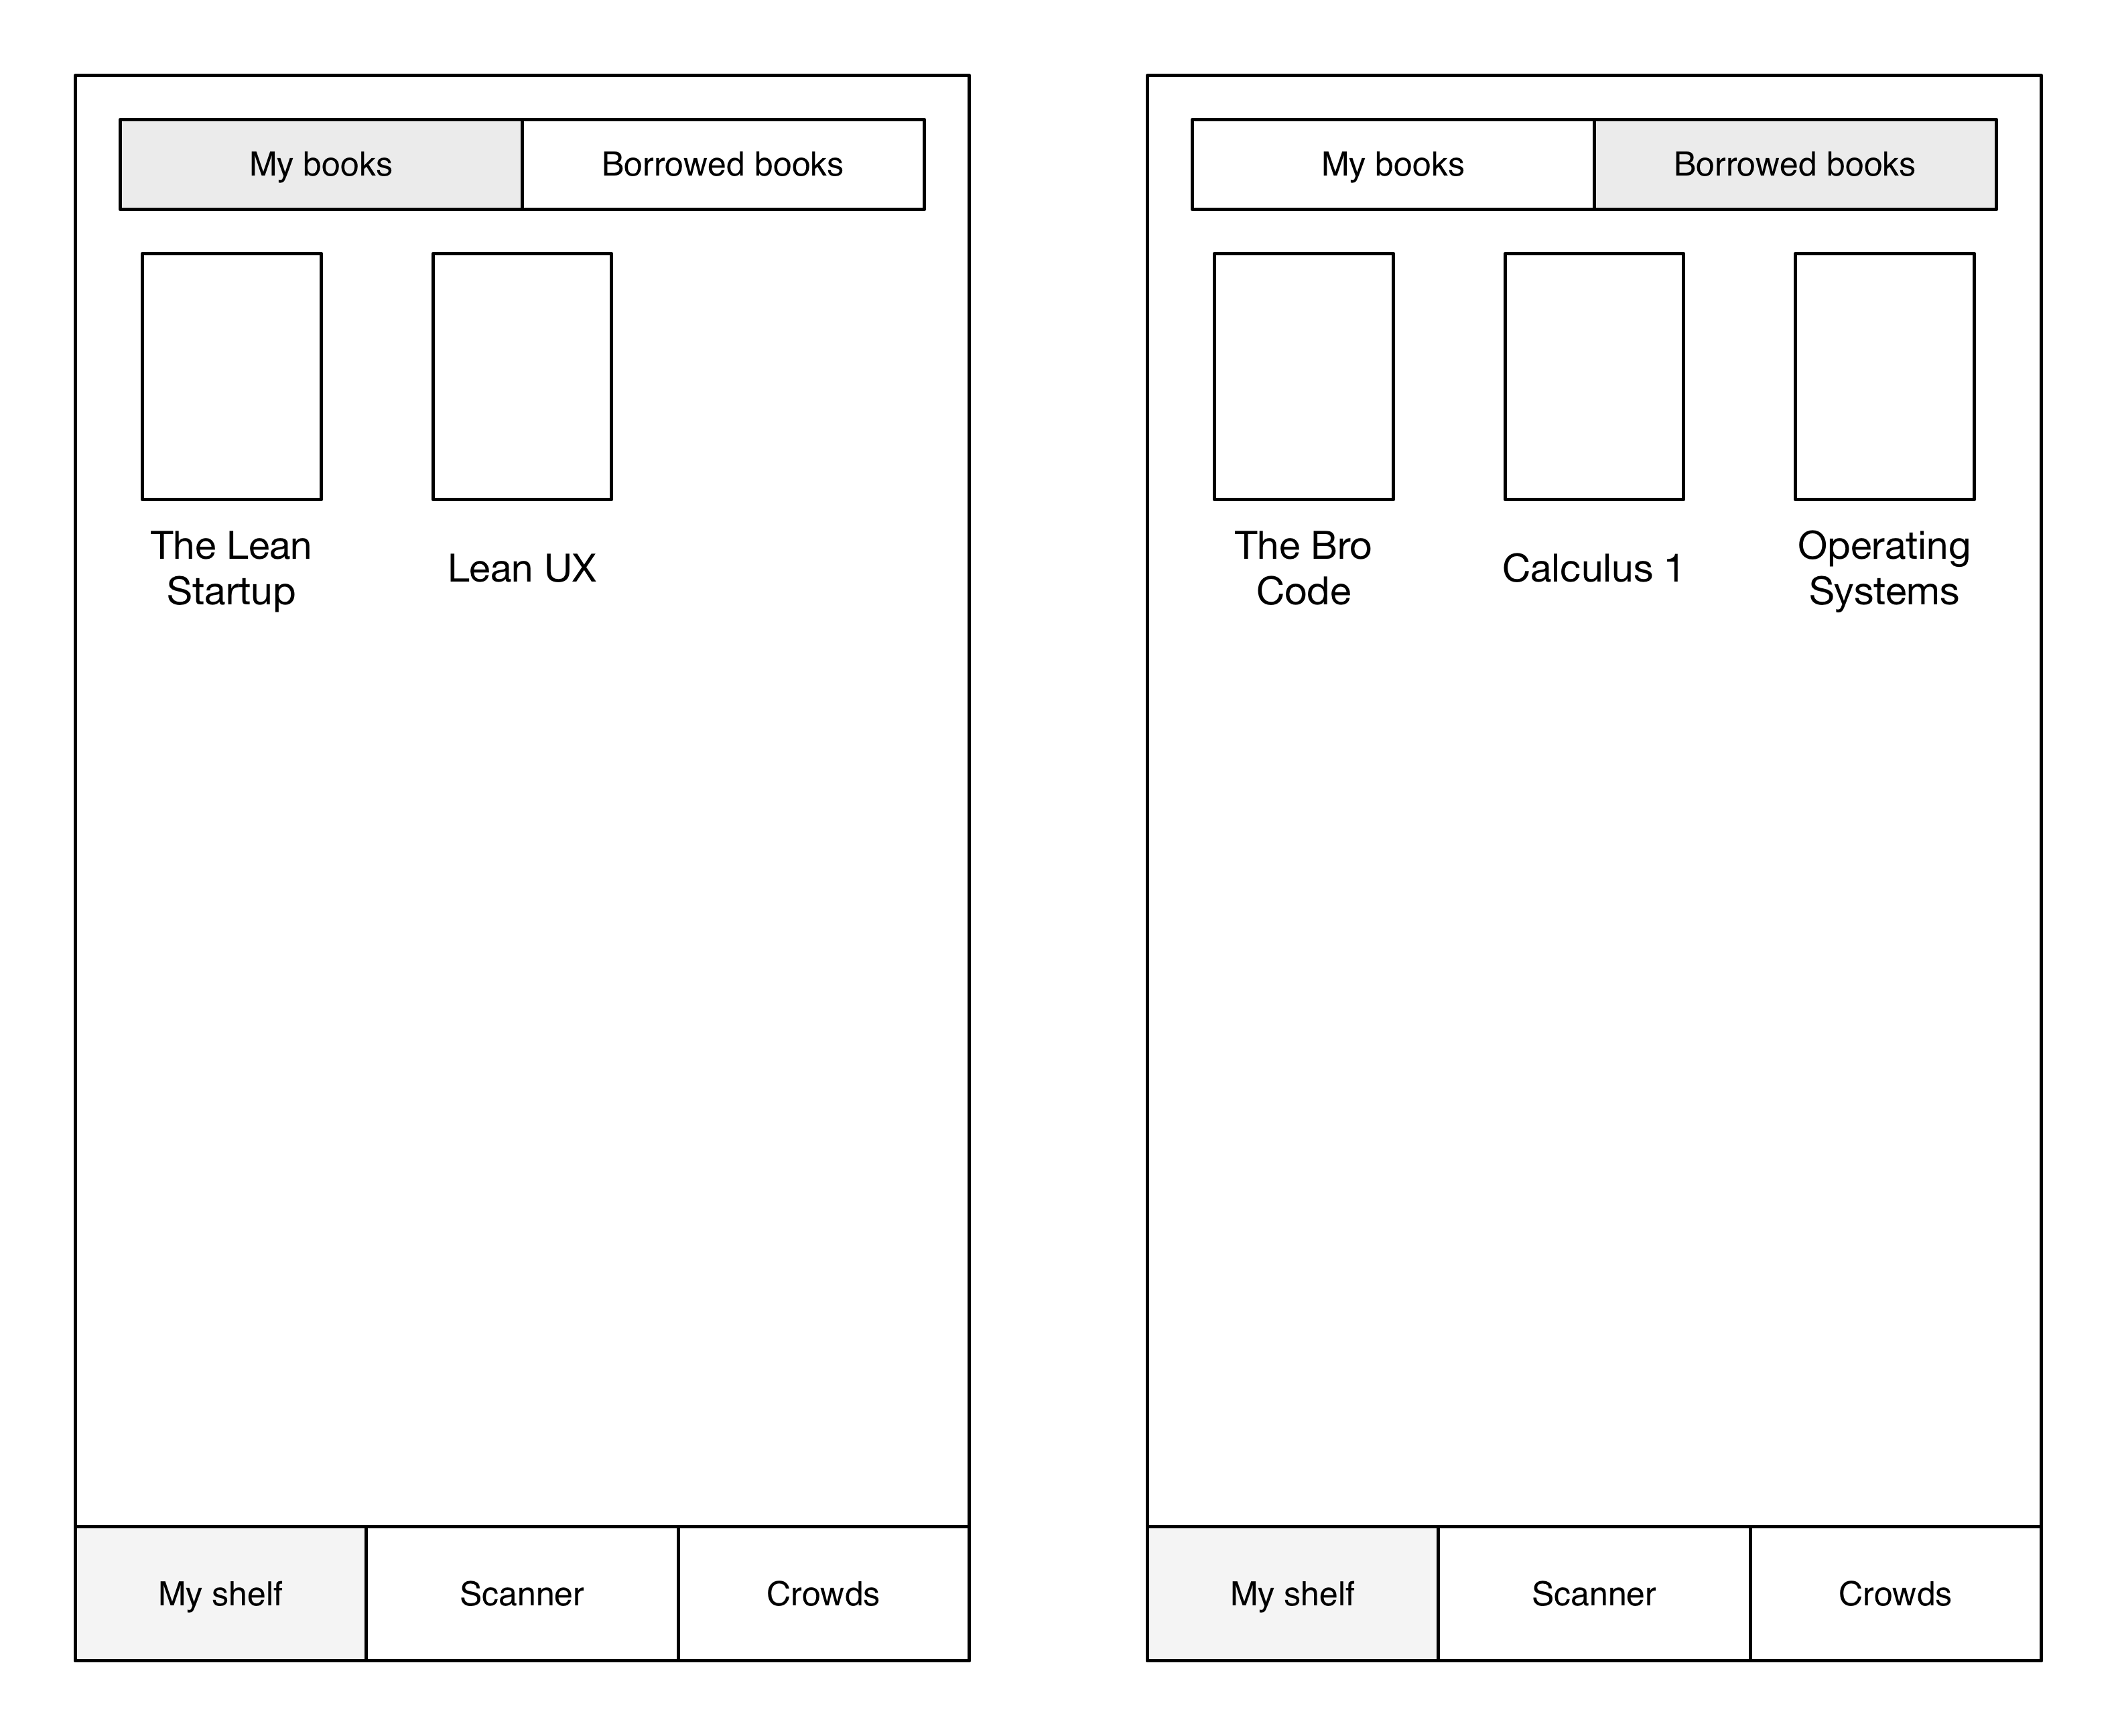
\includegraphics[height=5cm]{figs/v04/Shelf.png}
    \caption{The shelf view where the user can see all its books}
    \label{fig:ios-shelf}
\end{figure}

\begin{figure}
\centering
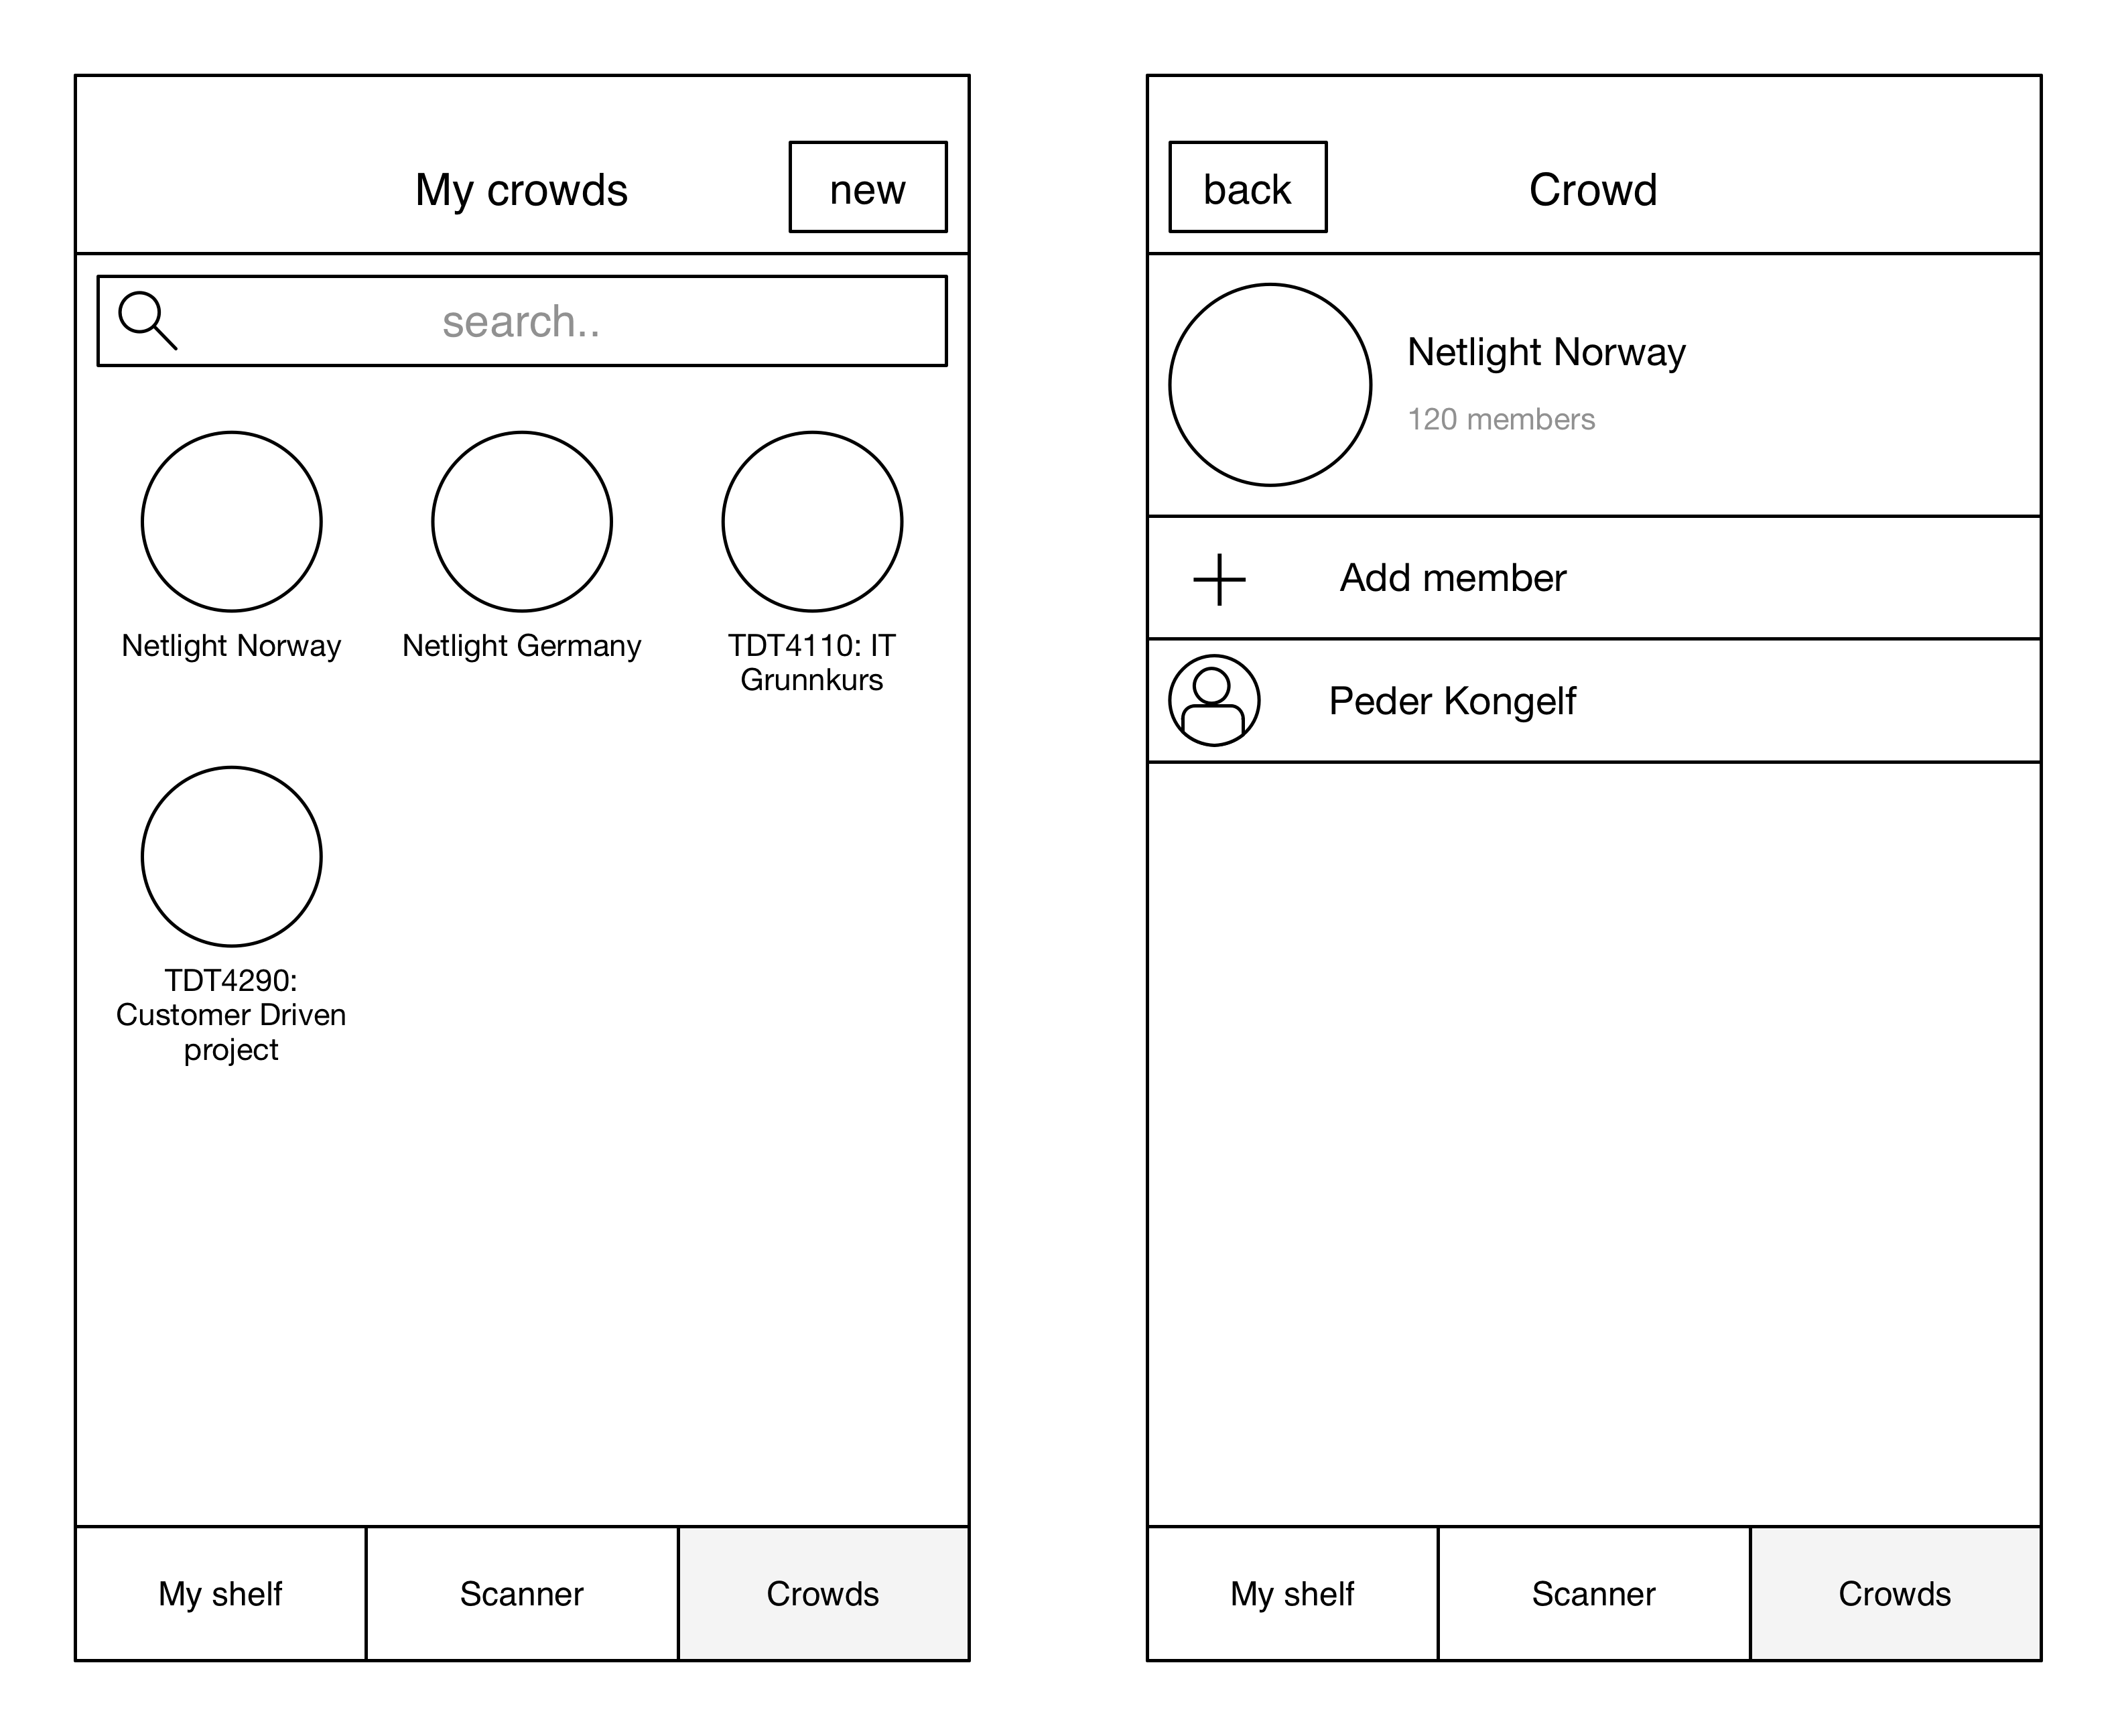
\includegraphics[height=5cm]{figs/v04/Crowd.png}
\caption{The crowd views where the user can see and manage all its crowds}
\label{fig:ios-crowd}
\end{figure}

\begin{figure}
\centering
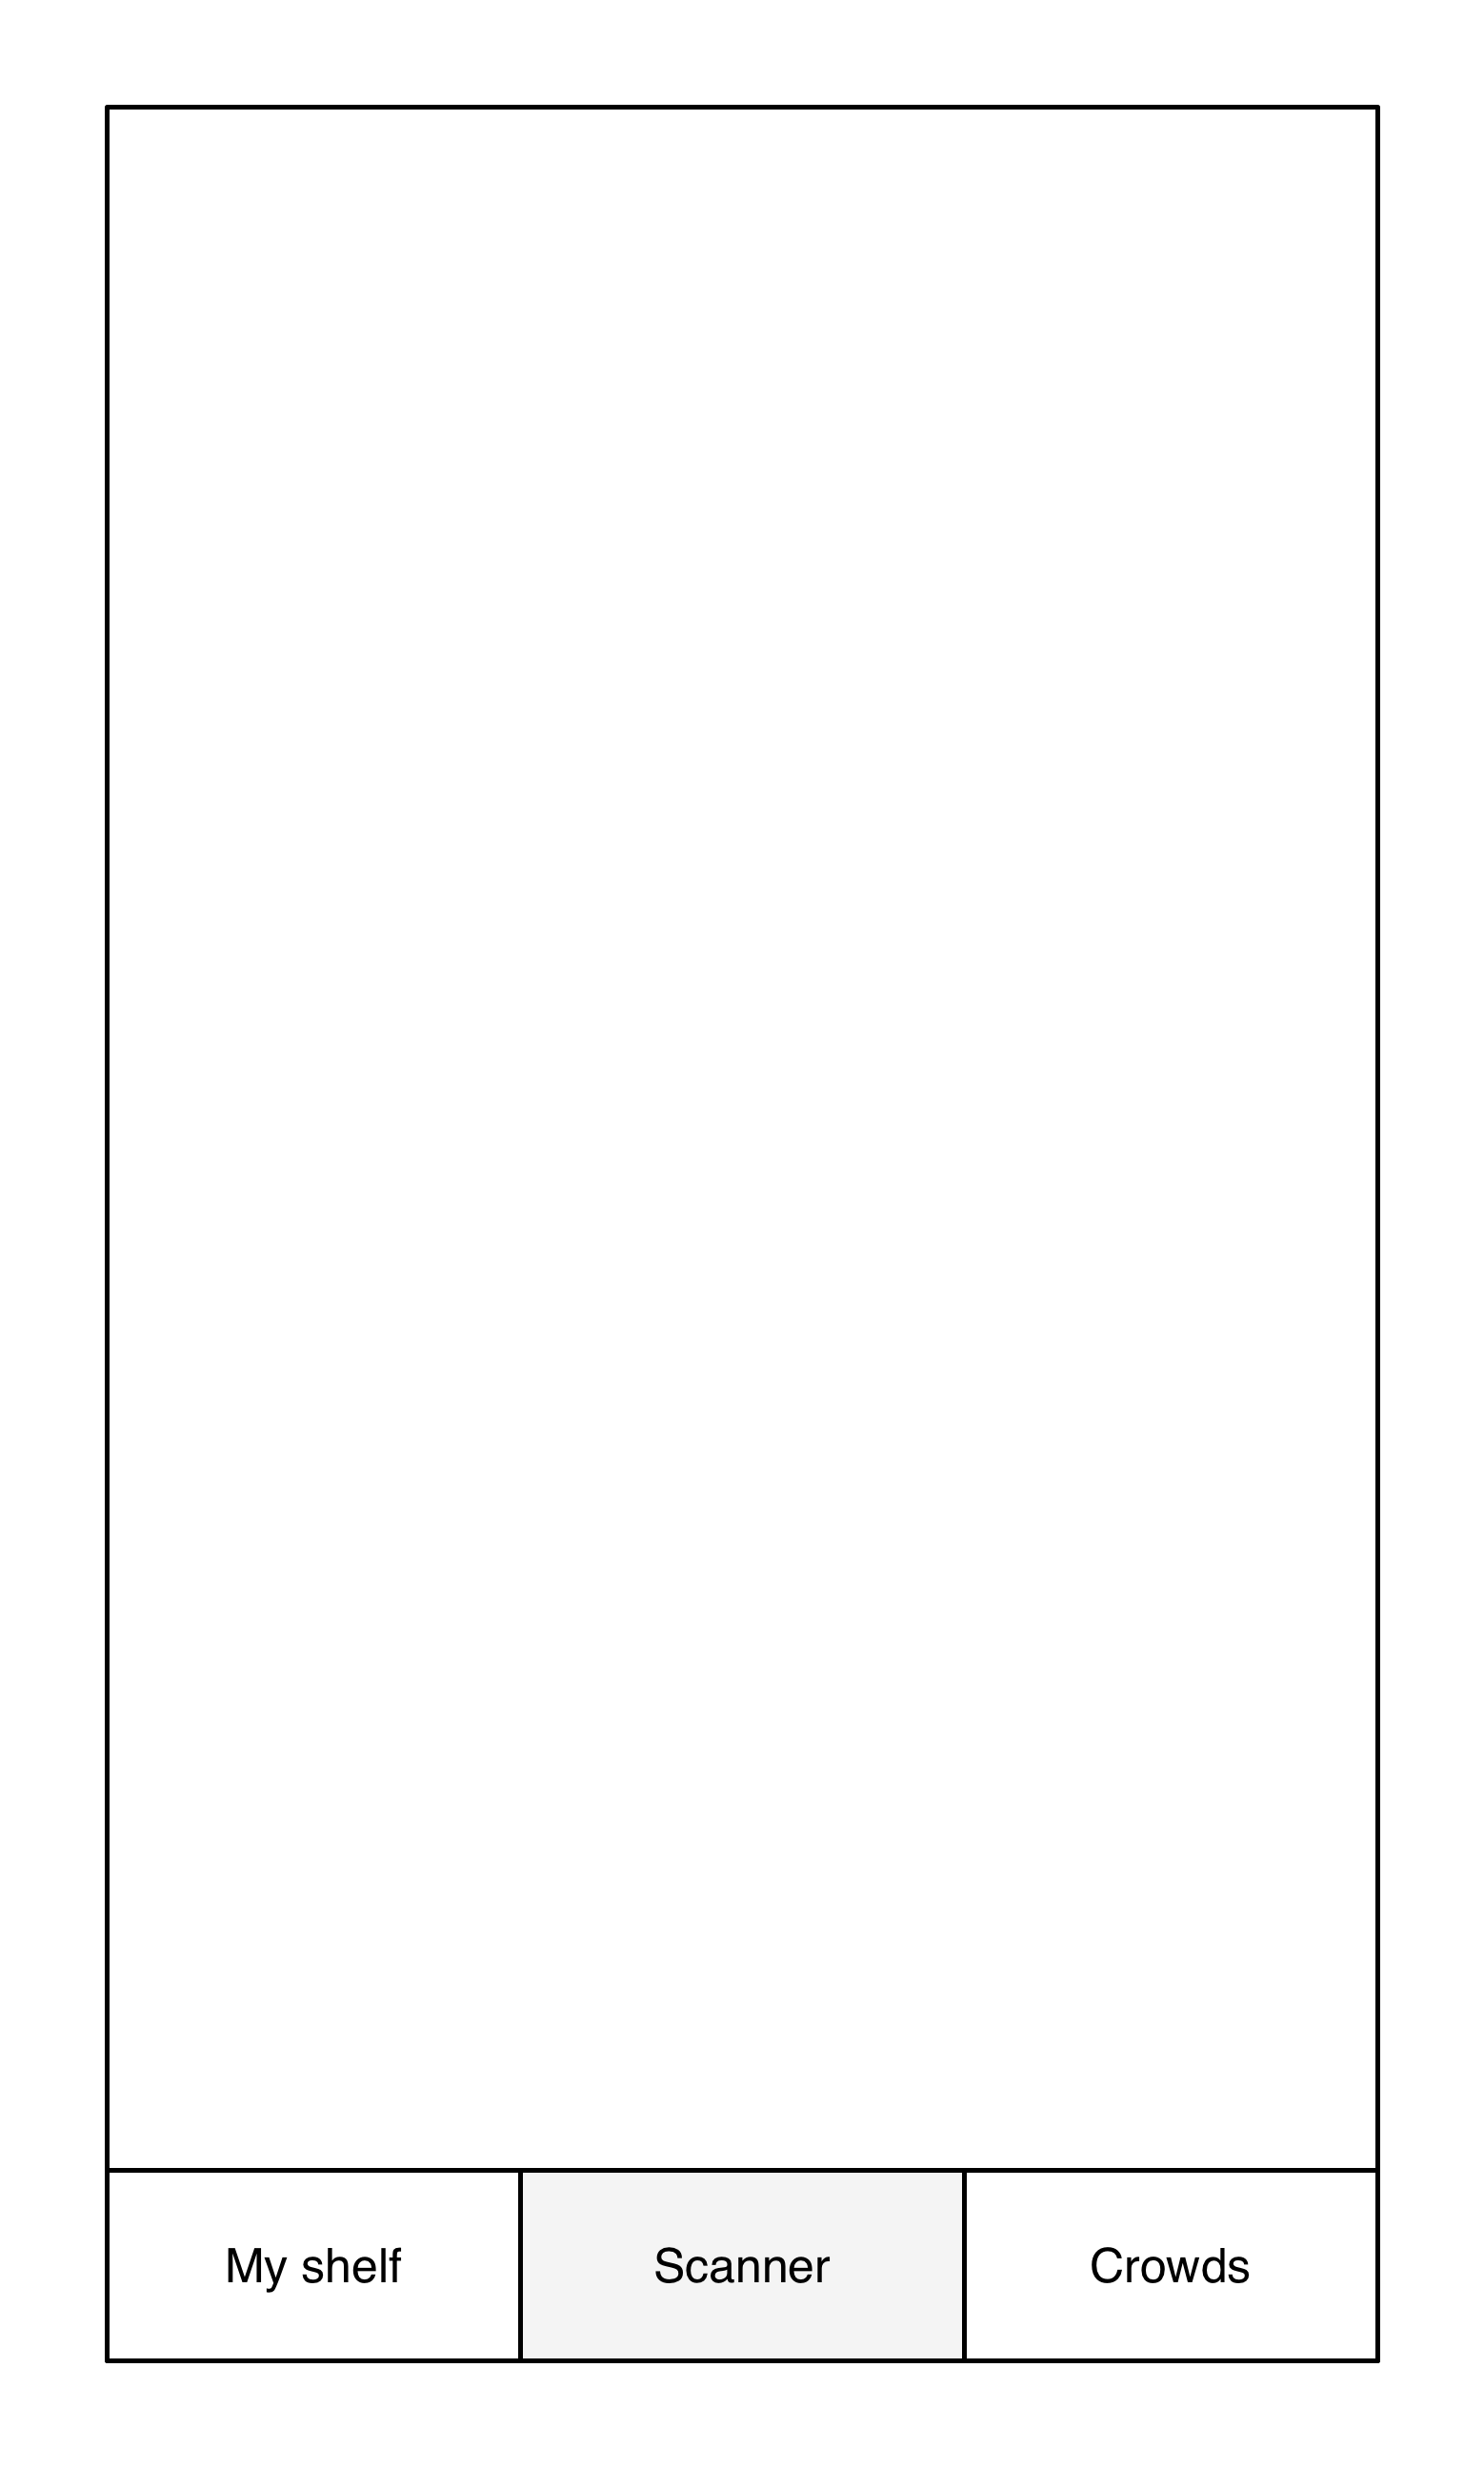
\includegraphics[height=5cm]{figs/v04/Scanner.png}
\caption{The scanner view where the user can scan the books' barcodes}
\label{fig:ios-scanner}
\end{figure}

\begin{figure}
\centering
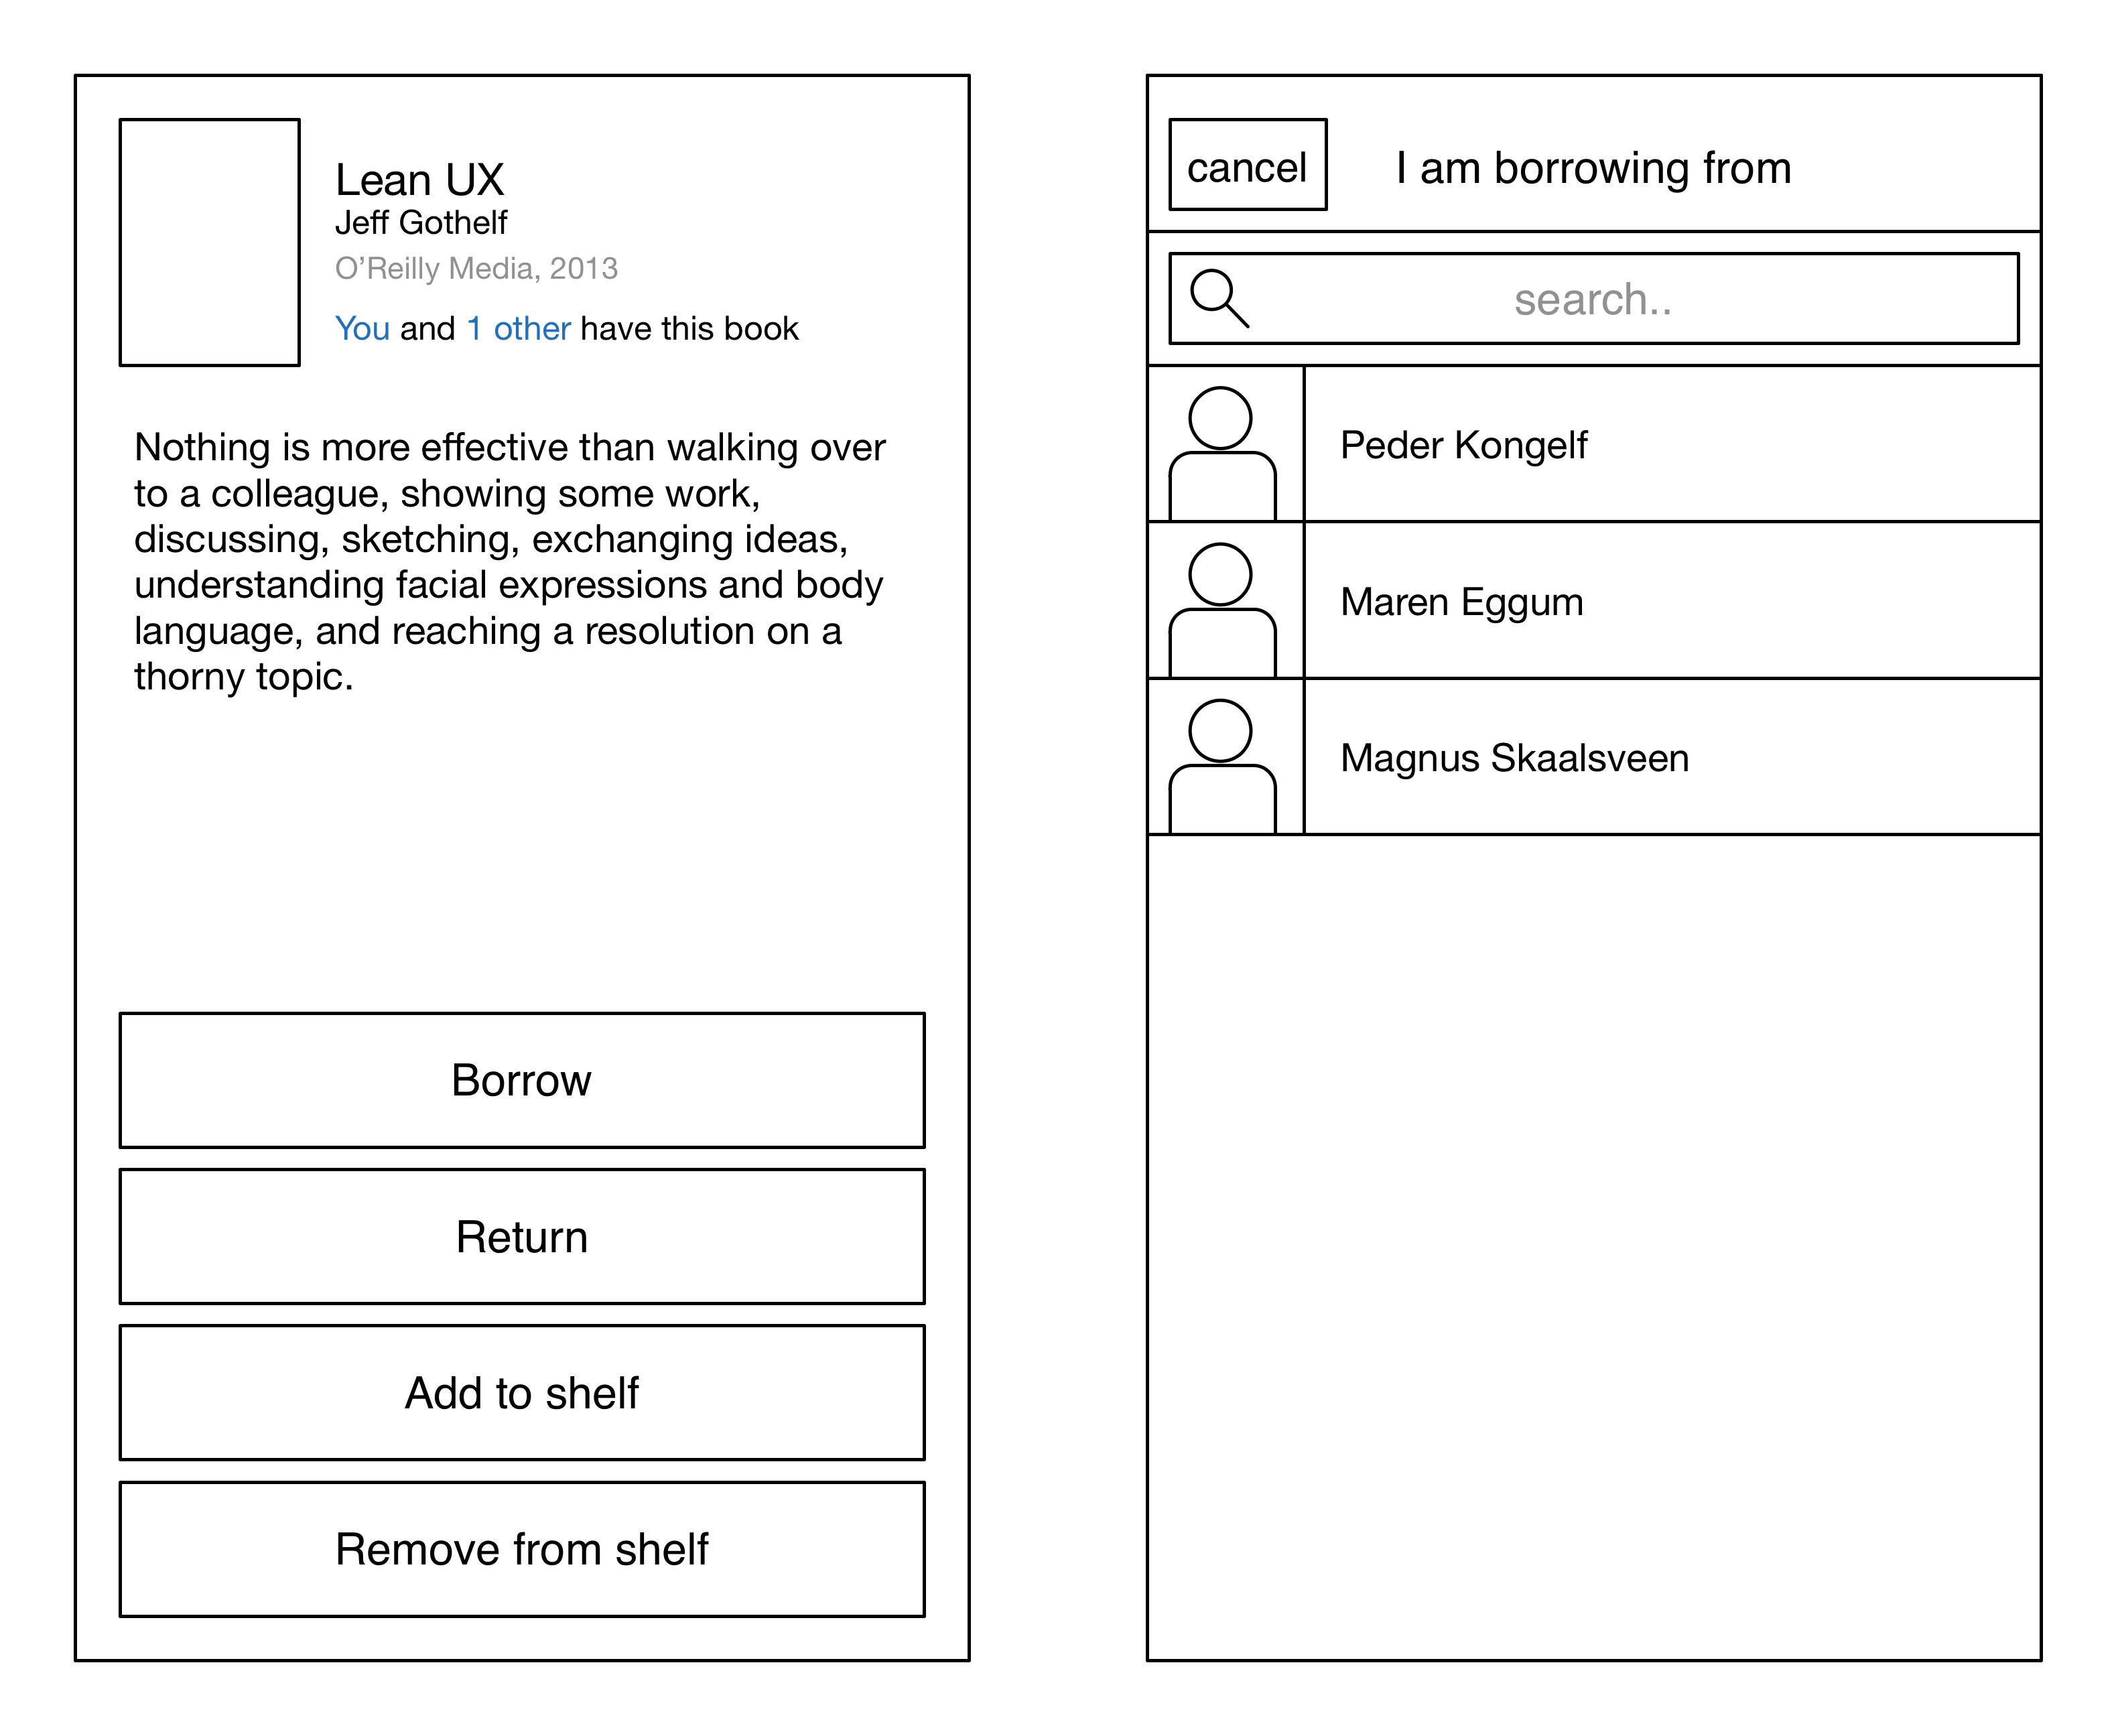
\includegraphics[height=5cm]{figs/v04/Book.png}
\caption{The book view where the user can see information about the book and add or remove it from its shelf.}
\label{fig:ios-book}
\end{figure}

\begin{figure}
\centering
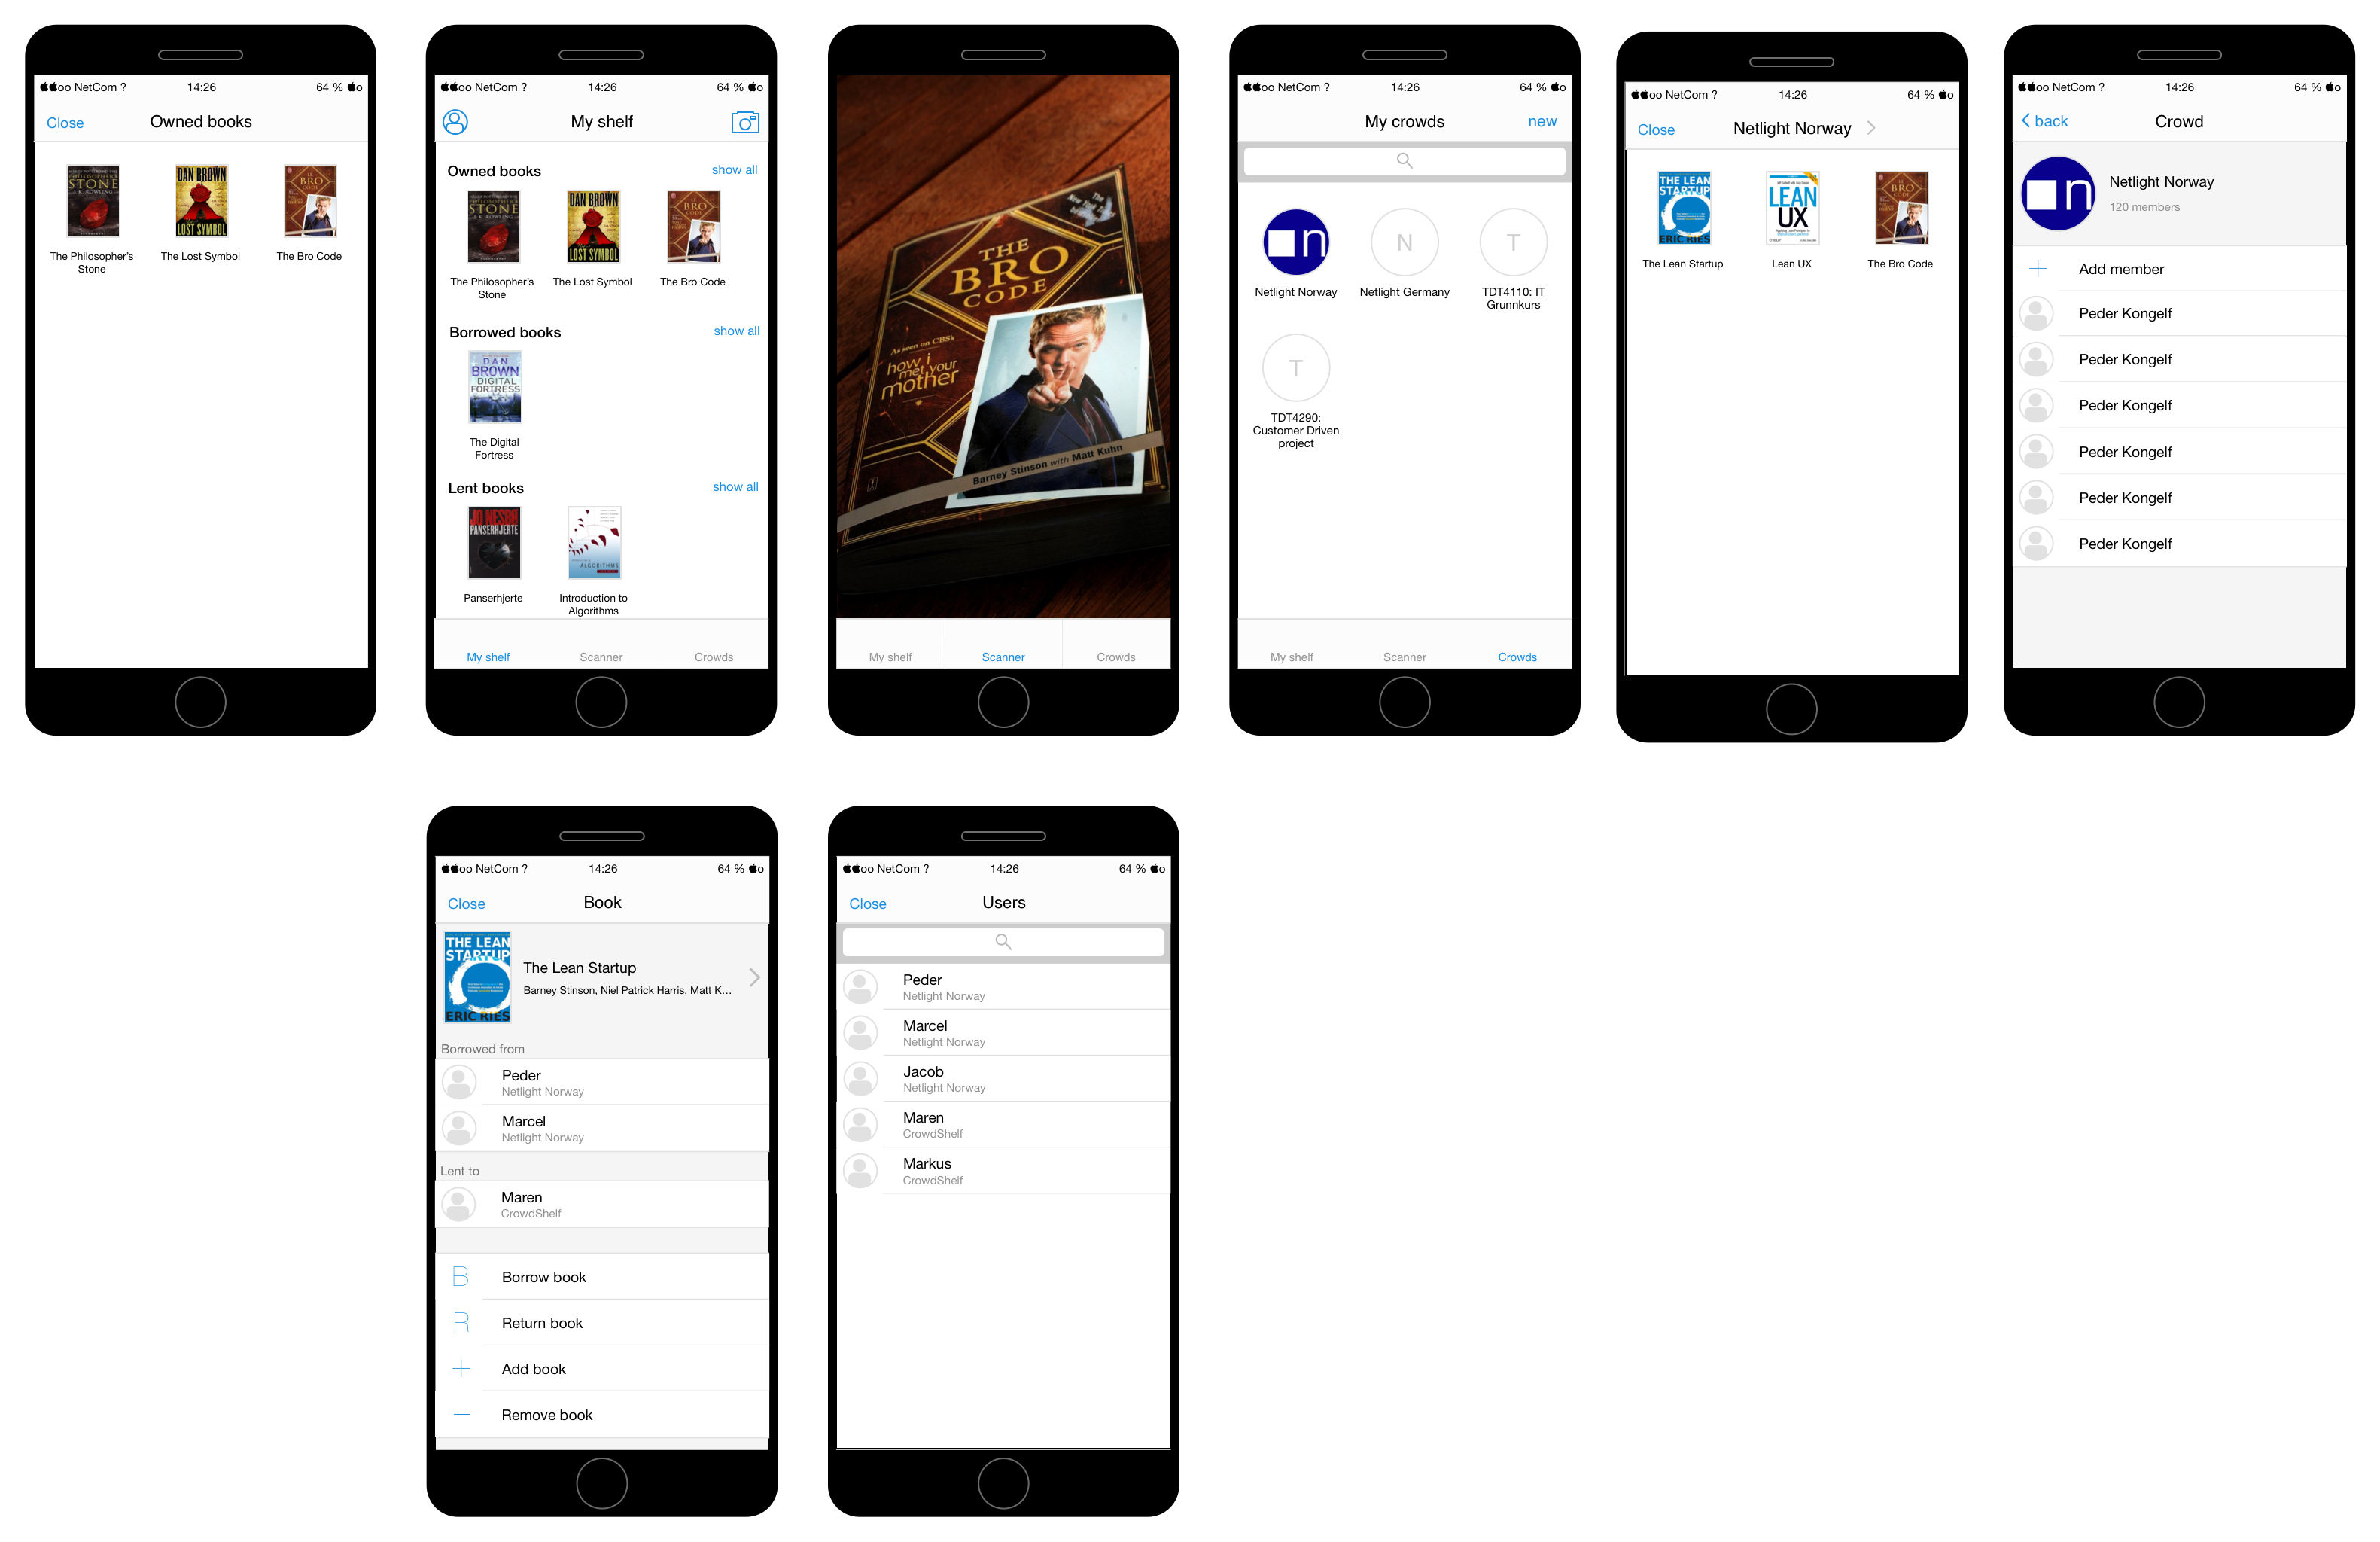
\includegraphics[width=14cm]{figs/v04/detailed-mockup.png}
\caption{A detailed design sketch}
\label{fig:design-sketch-4}
\end{figure}


\subsection{User stories}
\label{user-stories-v4}
This section shows the user stories selected as requirements version 0.4. The stories are selected based on the assumption thought to be the most relevant to test the new features 

\begin{enumerate}
  \item As a user I want to create a crowd
  \item As a user I want to leave a crowd
  \item As a user I want to see all books in my crowds
  \item As a user I want to see the owner and holder of all copies of a book in one/all of my crowds
\end{enumerate}

\subsection{Development}
The team has now gained momentum, and team communication flows better than ever. What this meant for the development of this version, is that the team could work faster. For instance, bugs in the \gls{backend} now fixed on the fly, as the other development teams notified the \gls{backend} lead what was wrong, and the the \gls{backend} team fixed it.

\subsubsection{Android}
\begin{description}
    \item[Features] \hfill\\
The biggest feature of this version was the ability to create new crowds and manage which users that were members of different crowds. A user could be added to a specific crowd by adding a user's username to the crowd, and a user could be a member of multiple crowds. This allowed the user to be able to borrow books from other users in the same crowds. This feature required the application to have a view that could display which crowds a user participates in, and also a view for the creation and management of crowds. 

    \item[Structure] \hfill\\
A new fragment was added to the \code{MainTabbedActivity} activity, which now consisted of three fragments; the user's shelf, the scanner and the new crowd list fragment, \code{CrowdScreenFragment}. See figure \ref{fig:AndroidStructure-04}. The new crowd fragment showed a list of which crowds the user was a member of. It was also possible to click on a crowd to open a new screen where the user could manage crowd details such as name and members. 

\begin{figure}
\centering
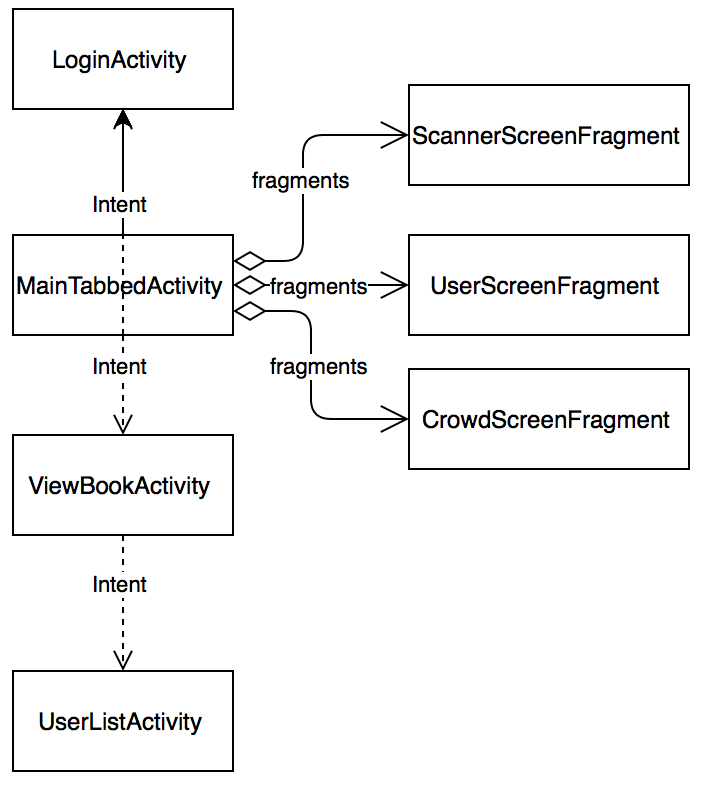
\includegraphics[height=7cm]{figs/v04/AndroidStructure-04.png}
\caption{Basic Android version 0.4 structure}
\label{fig:AndroidStructure-04}
\end{figure}

    \item[Design] \hfill\\
There were not many design changes during this version since the new crowd feature got the teams attention. The team did however start to think about how the application could look, and decided that this was going to be focused on in the next version. One design change that was implemented was to show tabs for the different fragments. Before this version the user was forced to swipe left or right to change fragment, but by implementing tabs, the user could now just go straight to a fragment by tapping on a tab. The new tabs used for navigation can is shown in figure \ref{fig:AndroidDesign-04}

\begin{figure}
\centering
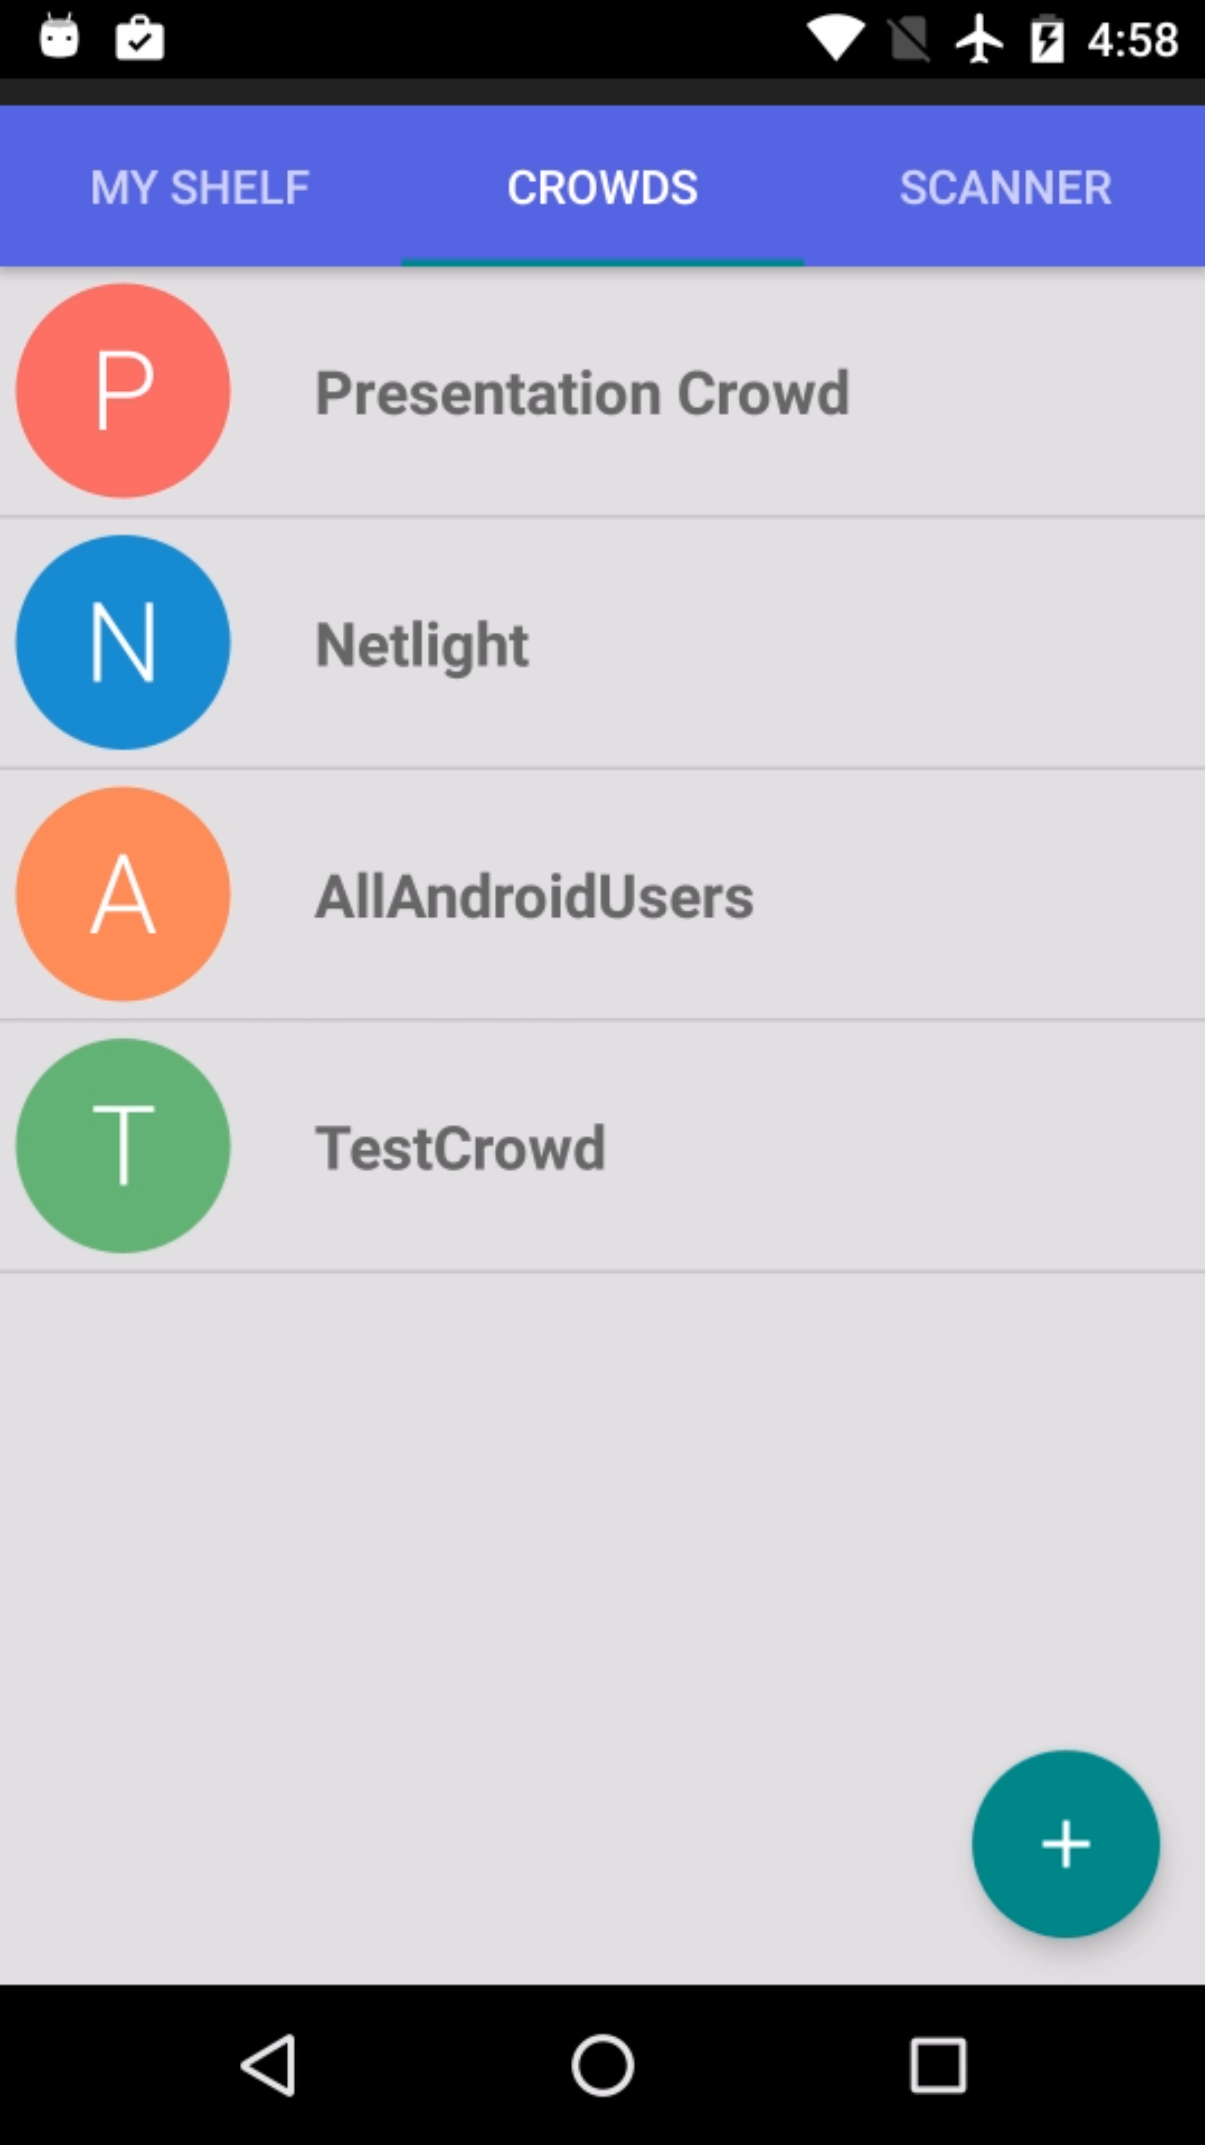
\includegraphics[height=7cm]{figs/v04/AndroidDesign-04.png}
\caption{Android version 0.4 design}
\label{fig:AndroidDesign-04}
\end{figure}

    \item[User feedback] \hfill\\
The new feedback the team wanted to track in this version was if the users used the new implemented crowds functionality.The team then chose to track when a crowd was created, when a a user left a crowd, when a crowd was deleted and when a member was added to a crowd. See table \ref{tab:mixpanel_table} for a full overview of event that got tracked.

    \item[Bug fixes] \hfill\\
The application was made faster on startup by only downloading book information that is not already stored in the local realm database. Another bug discovered was that if a user launched the app, closed it and launched it a second time the application crashed. The reason for this bug was that not all instances using the realm database closed the connection to realm when the instance was finished with communicating with realm. This was solved by making the activities and instances using realm close the connection to realm when the instance was closed or destroyed.
\end{description}

\subsubsection{iOS}
\begin{description}
    \item[Features] \hfill\\
The main feature for this version was to enable users to select which users they wanted to share their books with. This was done by allowing them to create groups and invite other users they trusted. All books a user owned would be shared in all groups they were a part of. In order to achieve this a few new views would have to be created. A new view where the user can see all the groups it is currently a member of, or create new group, and a view with detailed information about the books and members of a given group. 

The network handler had to be updated with methods for creating and removing groups, adding and removing members of a group, and updating information such as the name. 

    \item[Design] \hfill\\
The design of the new views were based on the updated design created after a series of usability tests.

    \item[Feedback] \hfill\\
The integration of Mixpanel from version 0.4 was extended to also include reporting the creation, update and removal of groups. This would allow the team to monitor how the new features were used.
\end{description}

\subsubsection{Backend}
\label{sec:backend-v0.4}
This iteration the team kept up with the other development teams to fix bugs, but most of the time was spent learning about Docker, and creating a Docker-image. \cite{docker} The team managed to write a Docker-file that was used to build a Docker-image. For more information on Docker, see the preliminary studies, section \ref{prelim-docker}. How the Docker-image can be fetched and run is descirbed in the developers documentation to the backend, which is the readme-file of the GitHub-repository. This can be found in appendix \ref{app:backend-readme}.

The team went on to learn about Docker Hub, where you can share Docker-images. \cite{dockerhub} There the team created our own organization page, and a project for the server. \cite{dockerhub-crowdshelf}. The team built the an image for the server application, and pushed it to the Docker Hub. 

Docker Hub lets one can connect with GitHub, so that it detects when someone pushes new code. If the GitHub-repository has a Docker-file, Docker Hub can automatically build a new image and also send HTTP-requests to other services, which in turn can have listeners in place for pulling the image and restarting it's services. \cite{dockerhub-builds} The team set this up so that Docker Hub automatically built a new image whenever there was changes to the \code{master}-\gls{branch} on GitHub.

 In the previous iteration the team bought the domain \url{crowdshelf.xyz} and pointed it to the virtual machine running with Digital Ocean. In this iteration a team member wrote a small application\cite{essoen-dockerpuller} based on one found Online \cite{dockerpuller} that could take in a HTTP-request and based on that call a shell-script. A team member wrote a shell script that could pull the Docker-image from the Docker Hub, and restart it. See code-listing \ref{shell-script} This was set up on the server, and the Docker-image was pulled from the Docker Hub. On the Docker Hub web page the team added a web hook, so that when someone pushed a new version of the Docker-image to the Docker Hub, the Digital Ocean machine automatically pulled the new image, and started it.

In other words the whole deployment process was standardized and automated around the Docker platform with version 0.4.

\begin{lstlisting}[float,floatplacement=H,frame=single, columns=fullflexible, caption=Shell-script used by the virtual machine running at Digital Ocean to restart the server application with Docker when there is deployed a new version, label=shell-script]
    docker pull crowdshelf/server:latest
    docker stop crowdshelf
    docker rm crowdshelf
    docker run --name crowdshelf --net host crowdshelf/server:latest
\end{lstlisting}


This version was also spent discussing a possible new service that was to be developed: A Book Service. A web developer from our customer wanted to build a web application on top of the CrowdShelf \gls{API}. The problem here was that the web application did not have local storage, and therefore had difficulties cashing the data from the Google Books \gls{API}, that the mobile applications used for meta information. The web developer also claimed that the Google Books \gls{API} had some limitations as to how many requests one could run. The customer requested that the team developed a new service that could save Google Books-data, and connect it with the already existing \gls{backend}. The team also found that the \gls{backend} could be a service to save books that were not anywhere else. The customer representative also suggested that other types of items could be saved in the service, which in turn could be used to extend the market of the application. 

The team developed a specification for an \gls{API} together with the customer representative that could meet the above mentioned needs. The team soon found it to be very complex. If one would have Google Books references in an own database, and a reference to them from the already existing \gls{backend}, a lot of validation had to be implemented. The backend team also had some difficulties seeing the need of the web developer. The problem she had, did not indicate that she would need a new service. The mobile application developers did multiple requests to the Google Books API, and met no limitations, while the web developer claimed she did. The team found that this may have to do with a limitation the Google Books \gls{API} had with searching their databases. The team could request resources directly as much as as the team wanted.

After a final meeting with the customer representative, the \gls{backend} team an the customer finally decided to scrap the plans for the service, as it would be too complex and costly to develop in the time frame of the project. 

\subsection{Feedback}
Feedback from the survey (appendix \ref{app:0.4-survey-feedback}) was a clear indication that users want some way of restricting the access other users have to their virtual library. Only 6 \% were willing to share their books with strangers, but 80 \% wanted to share books with friends and colleagues. This seemed to support the theory that allowing users to create groups, in which they could share their books, was a demand rooted in future user needs.


The results from the usability tests were highly dependent on the user group in question. All students had no problem navigating the application, and completion all tasks. This could be a consequence of the design being based on Facebook's Messenger application design, which  students probably use more than most other user groups. The employees at \gls{IDI} had some trouble understanding the applications in the beginning of the test. In particular, they had a hard time understanding that they could interact with the tab bar. As soon as they realized this, all but one completed the rest of the tasks without hesitation. 


The last tester did not manage to complete any task, and spent a long time just looking at the views. There could be many reasons for this. Perhaps she was having trouble understanding the concept of a paper prototype test, did not understand the basic concept and purpose of the application, or simply did not understand how to use the application the team presented. As no other users have expressed that they do not understand the most basic concepts of the solution, the team assumed that the latter was the most likely. Therefore a new design was created where some of the buttons were made more prominent. 


Like in previous versions, the applications were uploaded to Google Play and TestFlight, but very few users ever downloaded or installed them. During the customer meeting, the customer representative seemed satisfied with the result of the version, so the team continued the effort in developing a minimal viable product. Before this is achieved, there will be no usage data to measure.

Minutes from the customer meetings are located in \ref{app:customer-minutes-8} and \ref{app:customer-minutes-9}.


\begin{figure}
\centering
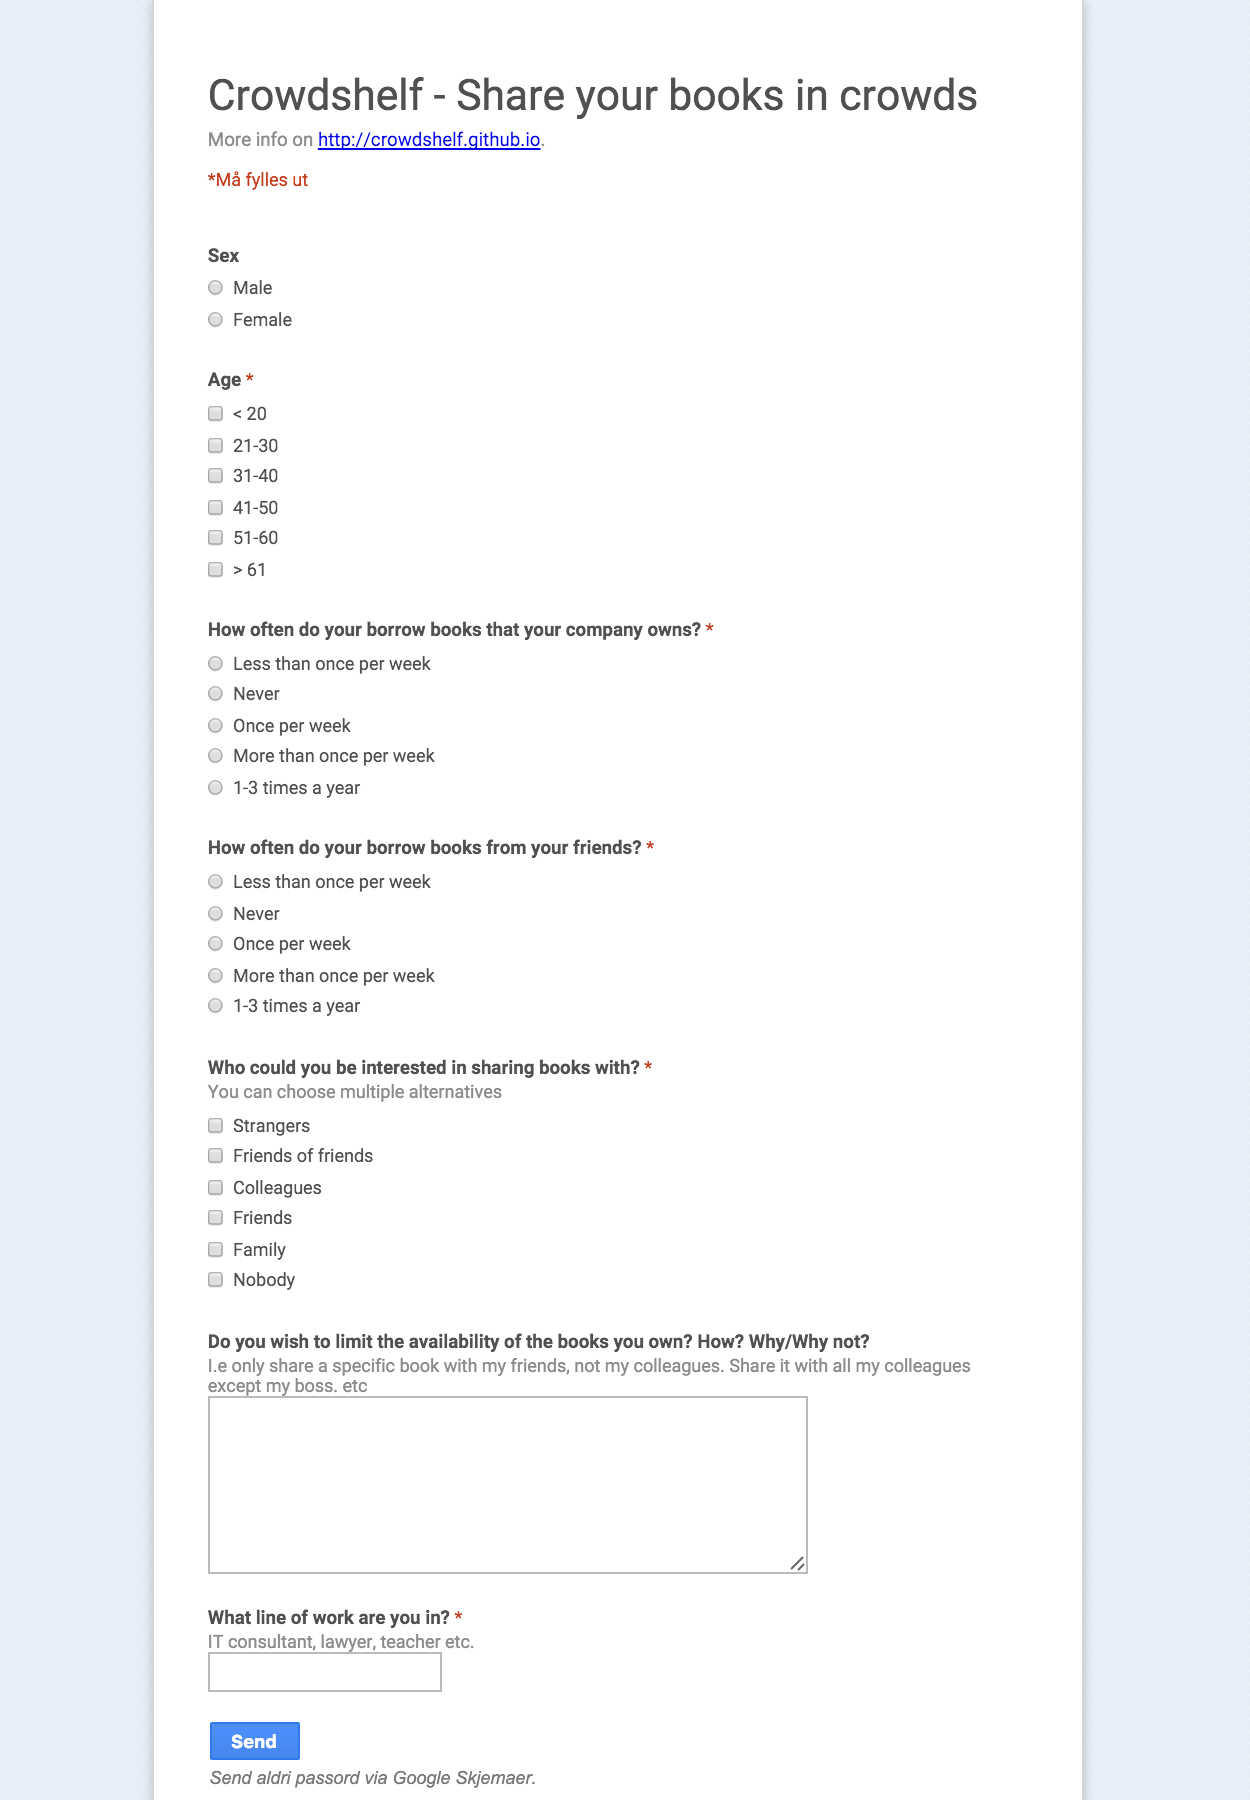
\includegraphics[height=\textheight]{figs/v04/survey.png}
\caption{The survey used to gather necessary information from potential users}
\label{fig:0.4-survey}
\end{figure}

\begin{figure}
\centering
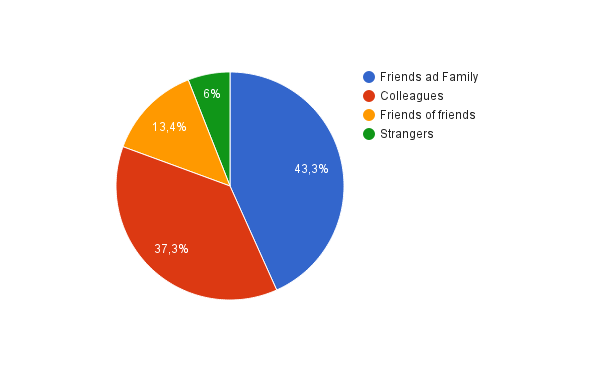
\includegraphics[width=\textwidth]{figs/v04/feedback-pie.png}
\caption{A pie chart illustrating the percentages of people willing to share with certain groups}
\label{fig:0.4-survey-feedback}
\end{figure}


\subsection{Version progress}

With the completion of this version, the application is one step closer to being ready for distribution. The crowd feature enables users to choose how they want to share their books. The progression during this iteration is illustrated in figure \ref{fig:0.4-survey-feedback}. A complete list of all tasks from this version can be seen in the release note in appendix \ref{app:release-note-4}

Although no serious problems were encountered, this iteration lasted more than a week due to the delivery of a mid-term report. A few days were spent solely on preparing the report which lead to a halt in the development on both the clients and the backend. 

A new blog post was written and is displayed in figure \ref{fig:blog-week-eight}

\begin{figure}
\centering
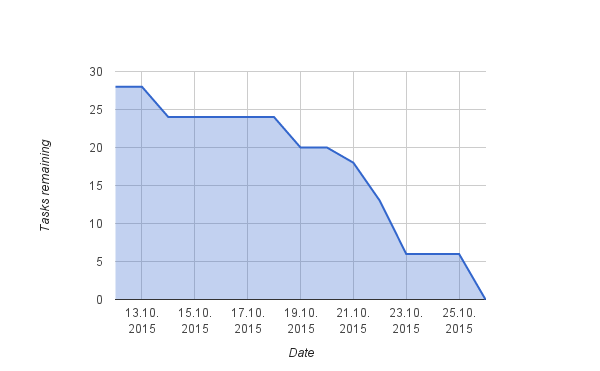
\includegraphics[width=\textwidth]{figs/v04/version-progress-4.png}
\caption{Task progress version 0.4}
\label{fig:version-progress-4}
\end{figure}

\begin{figure}
\centering
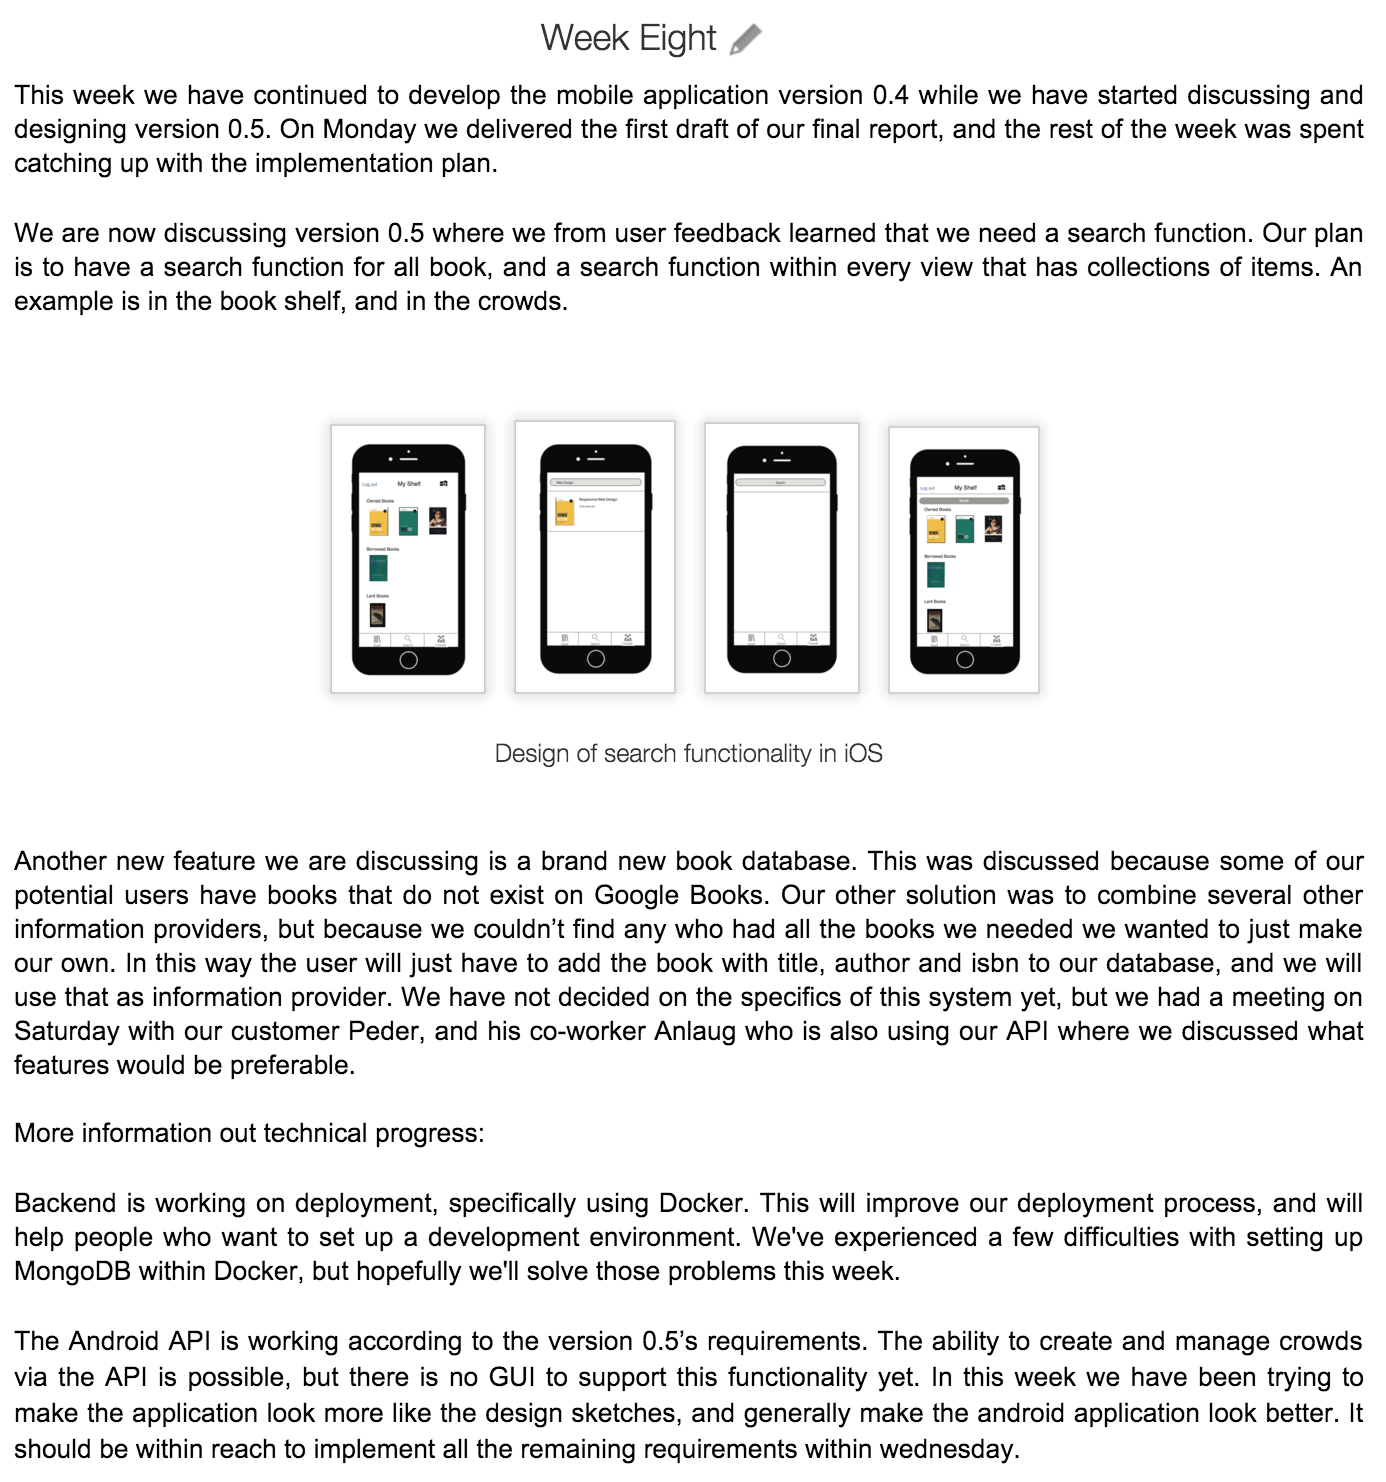
\includegraphics[height=20cm]{figs/v04/WeekEight.png}
\caption{Blog post from week eight}
\label{fig:blog-week-eight}
\end{figure}

\subsection{Review and retrospective}

At the end of the iteration, the mobile applications and \gls{API} were presented to the customer. For Android and iOS, a couple of videos demonstrating the crowds feature were made. The customer representative seemed pleased with the solution, but he suggested that the team should attempt to establish a vocabulary to ease the communication when discussing subjects such as groups, end points, and crowds. He also wanted the demonstration videos to contain books which a broader audience would recognize, and use crowd names that could help the viewer understand how the crowd feature can be used. The minutes from the customer meetings is located as appendix \ref{app:customer-minutes-8} and \ref{app:customer-minutes-9}.

Because the final delivery was merely two weeks away, the customer representative shared what his functional requirements for the end result were. I addition to the existing features, it needs to be possible to search for books using raw text. This could be done using the Google Books API, but it should be possible to filter the results to contain only books from the users crowds. The last requirement was that users had to be authenticated in order to restrict what data a people have access to. At the moment, everyone has access to all information in the database provided they have the necessary usernames and \gls{ISBN}s. These features should be implemented during the last two iterations.

The focus points of this iteration were to become better at using Jira for tracking issues, and connecting our results to the initial assumption. All team members agreed that during the this version, they had become better at using Jira, and could now see the connection between the assumptions and results.

\begin{figure}
\centering
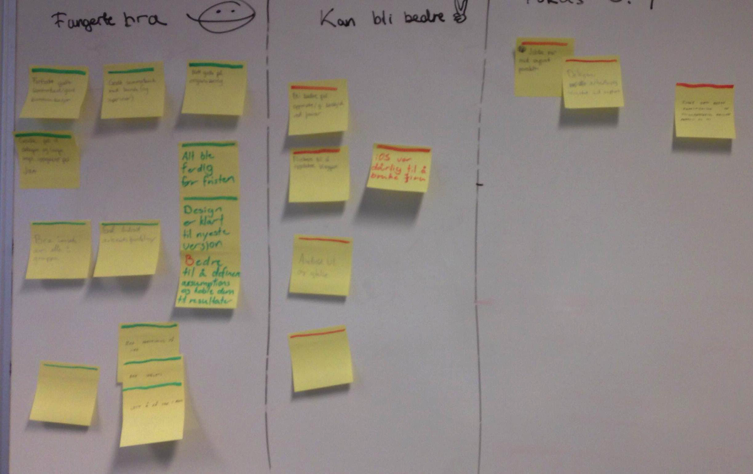
\includegraphics[height=8cm]{figs/v04/retrospective.png}
\caption{The board after the retrospective meeting in version 0.4}
\label{fig:retrospective-4}
\end{figure}


\subsection{Summary}
The initial assumption for this version was that users only want to share books with a selection of users. Even though users said that they do not want any restrictions on their books, the survey was a clear indication that they do not want to share with strangers. This told the team one of the lessons learned this version: users want to restrict who can borrow their books.

The crowd functionality was implemented on the clients and on the server based on this knowledge, and then distributed to users through Google Play and TestFlight.\cite{google-play}\cite{testflight} When usage data is received, question eight can be answered as well.


\section{Version 0.5}
In the fifth version the goal was to learn if it would be beneficial for the user to have another possibility to find books other that scanning the barcode of a book. Indications received from the customer and other users suggest the need of this functionality, and it was therefore selected as the assumption of this version. 
\subsection{Assumptions and questions}
The assumptions to be confirmed in this iteration was “Users want to be able to search for book by text”.

Questions used to verify this assumption:
\begin{enumerate}
    \item How are the users used to search in applications?
    \item On what type of information do the users want to search?
    \item What are the users interested in being returned from the search?
\end{enumerate}

\subsection{Planning and design}
Defining how to get answers to these questions was the first part of planning the version. Fortunately the indication that this was a desired feature had already been received from the customer representative which meant that the team could start directly with the design of the new feature in the applications. 

In the customer meeting held the day before this version, the customer representative had stated that both search and user validation was needed for the application to be a real \gls{MVP} that he could distribute to the employees at Netlight. Because the search functionality is a feature concerning the mobile applications, and the only support needed from \gls{backend} (filter on owners) was already implemented the \gls{backend} team would work on creating support for user validation (0.6) during this iteration.

To learn the answers to the first question, the team analyzed how some regularly used application like Facebook, Google Play for the Android users and AppStore and iBooks for the iOS users have implemented search functionality. In iOS the search is placed in the tab bar (bottom) shown in figure \ref{fig:ios-search-design}, while it is placed in the action bar (top) in the Android application.
\begin{figure}
\centering
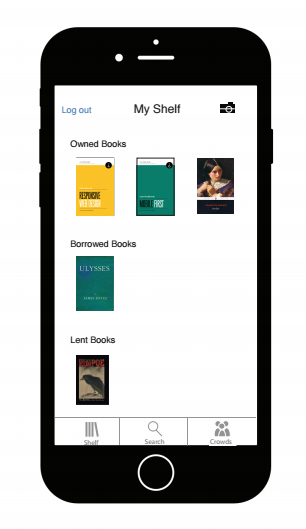
\includegraphics[height=7cm]{figs/v05/ios-search-design.png}
\caption{iOS design of search button}
\label{fig:ios-search-design}
\end{figure}


On the note of layout it was decided to renew the Android design during this version. Following the Android design principles, a new layout was defined. \cite{android-design} A color palette shown in figure \ref{fig:color-palette} selected from Google’s material design color palettes was selected for the application. In addition, the design team studied the design principles and other android applications, and concluded on a design illustrated from the shelf view in figure \ref{fig:android-design}

\begin{figure}
\centering
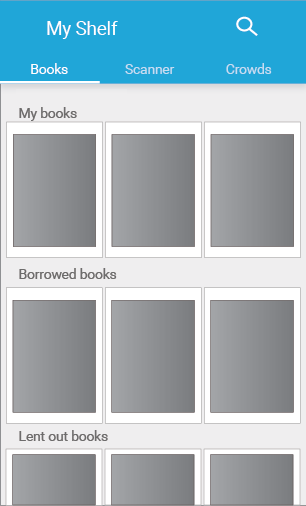
\includegraphics[height=6cm]{figs/v05/android-search-design.png}
\caption{The new Android color design with search button}
\label{fig:android-design}
\end{figure}

\begin{figure}
\centering
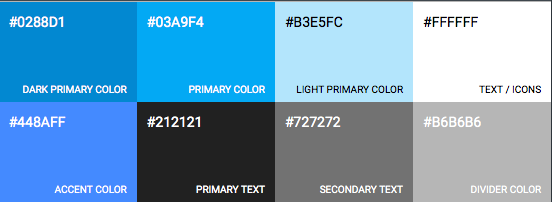
\includegraphics[height=4cm]{figs/v05/color-palette.png}
\caption{The color palette selected for the application}
\label{fig:color-palette}
\end{figure}

Question two and three was intended to be answered by the measurement of use in the application. In reference to the second question, the team decided that the users could search with any text they wanted, which would then search in Google Books and return that result. The team could then analyze what is searched using Mixpanel. This way if there are indications that the users do not get the results they want, for example if the same book is searched in different manners (author, title, ISBN) and only one of them returns a good result it might be preferable to let the users filter the search to what they are using to search.

The final question of what the users are interested in being returned from the search refers in addition to the design, to if they are interested in seeing all books, or just book owned by people in their groups. In the team it was decided to make both options possible by giving the user a filtering selection where they can choose between those two options. The team will then analyze what filter was used the most and make that the initial return of the search.

When planning this version the team decided to no longer use the term “Crowd” in the application, and instead use “Group” to describe the collections of users. This was decided in collaboration with the customer representative, and was discussed because the team had observed that some of the test persons from the usability tests had trouble understanding the meaning of a crowd.

After the measuring methods had been selected, three user stories were selected as the requirements needed to function in version 0.5. These user stories are shown in section \ref{user-stories-v5}


\subsection{User stories}
\label{user-stories-v5}
These user stories were selected to describe the functionality of version 0.5.
\begin{enumerate}
  \item As a user I want to search for books using ISBN
  \item As a user I want to search for books using title
  \item As a user I want to search for books using author
\end{enumerate}


\subsection{Development}
The implementation is still going well, and the teamwork has been great. The development for the different sub teams for this version is described in this section.
\subsubsection{Android}
\begin{description}
    \item[Features] \hfill\\
In version 0.5 the ability to search for books using text was implemented. The new search functionality allowed the user to choose between two different kinds of search, a local search in the user's groups and a search in the Google Books library. The search was implemented by adding a search button in the top right of the application's screen. When the user clicked on this button, a text field appeared next to the button, allowing the user to type in a search query. When the user confirmed the search query, it would search through groups the user was a member of in the realm database, and return a list of books that matched the search query. If the "search online"-button was clicked the application would search in the Google Books library.

Another new feature in this version was the possibility to view all the books a specific user is owning and all the books contained in a group. In earlier version of the application it was only possible to see if users had the book you were trying to borrow, not all the other books the user owned.

In the earlier version each book has been displayed as a different object, but in version 0.5 when choosing a book and viewing its information, information for all instances of the book was shown. This means that if a user had two copies of the same book and both were lent out, both renters would be shown in the book information. 

    \item[Structure] \hfill\\
In figure \ref{fig:AndroidDesign-05} a new activity has been added to the previous structure from version 0.4. The activity \code{SearchResultAcitivy} is the activity that handles how the search results from the user's search query are viewed on the screen. This activity also starts the \code{ViewBookActivity} activity if the user chooses a book from the list of books matching the search query, allowing the user the perform actions such as borrow or add on the selected book.

\begin{figure}
\centering
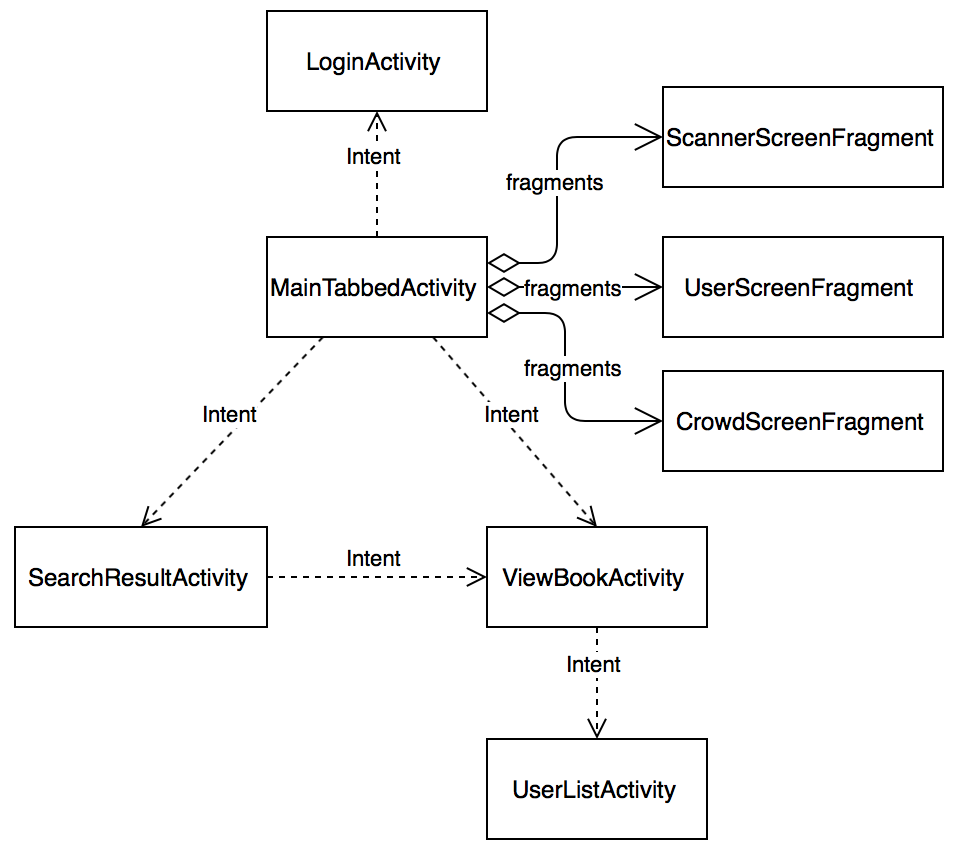
\includegraphics[height=7cm]{figs/v05/AndroidStructure-05.png}
\caption{Android version 0.5 structure}
\label{fig:AndroidDesign-05}
\end{figure}


    \item[Design] \hfill\\
Since the deadline for the project was approaching, the Android team decided to user more time on the design. They learned how it was possible to select a design and a set of color that should be used throughout the entire application. This means that if the team should decide to change the theme or color later they only need to do changes in one file. The team then used this design file to try to make the design follow the colors decided for the application. In figure \ref{fig:AndroidBookView05} it is possible to see how to book view have changed in this version (figure \ref{fig:androidcompare05}) from version 0.2 (figure \ref{fig:androidcompare02}).

\begin{figure}
\centering
\begin{subfigure}{.5\textwidth}
  \centering
  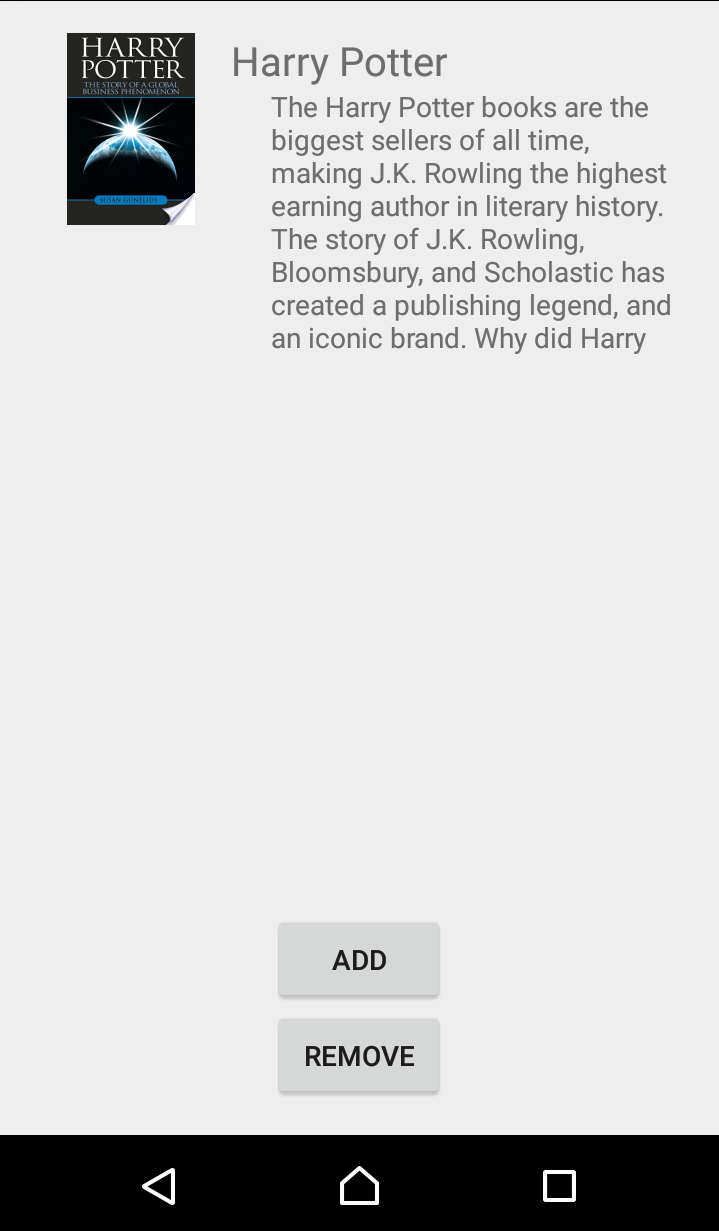
\includegraphics[width=.4\textwidth]{figs/v02/bookView02.png}
  \caption{Version 0.2}
  \label{fig:androidcompare02}
\end{subfigure}%
\begin{subfigure}{.5\textwidth}
  \centering
  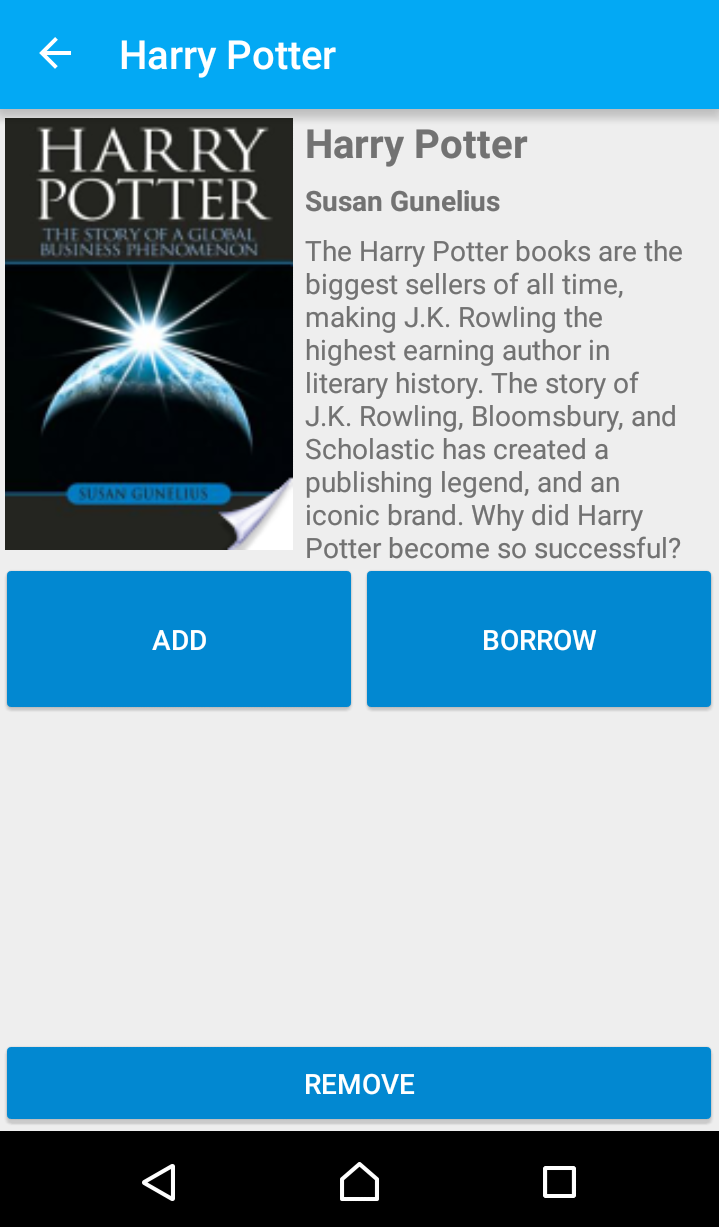
\includegraphics[width=.4\textwidth]{figs/v05/bookView05.png}
  \caption{Version 0.5}
  \label{fig:androidcompare05}
\end{subfigure}
\caption{Design changes from version 0.2 to version 0.5}
\label{fig:AndroidBookView05}
\end{figure}


    \item[User feedback] \hfill\\
In this version the team wanted to know if the users primary used search for searching in available books in the user's groups, or if the users used search to find books not already in the applications database to add these to their own shelf. To receive this feedback the event SwitchedFilter was added to Mixpanel, as shown in Table \ref{tab:mixpanel_table}. This allowed the team to track each time a user changed between local search and search in Google Books. 
\end{description}

\subsubsection{iOS}
\begin{description}
    \item[Features] \hfill\\
The iOS team spent this iteration implementing the new search feature, as requested by the customer. This was done sending a request with the users query to the Google Books API, and displaying the results as the user types. In an attempt to avoid the API's number of requests limitations, the requests were sent only after the query had been unchanged for at least 0.7 seconds. In order to filter the results to show only books in the users groups, a segmented controller was added to control the filter state. When the user selected the groups filter, a set of all available \gls{ISBN}s was compiled and used to filter the results from Google.

The shelf was also updated. It no longer show all the users unique books, but rather all the book titles the users owns. 

    \item[Design] \hfill\\
The team decided that moving the search feature in a dedicated view on the tab bar was the best approach for iOS. The existing scanner view was merged with the new search view in order to keep the tab bar clean and easy to use. To activate the scanner, the user had to navigate to the search view and press a camera button in the top, left corner. Search results were displayed as a list with the cover image and title of the book.

The scanner view was also improved with a rectangle showing the user where to position the barcode, and a new button which allows the user to activate or reactivate the device's torch for improved scanning in low light conditions.

\begin{figure}
\centering
\begin{subfigure}{.5\textwidth}
  \centering
  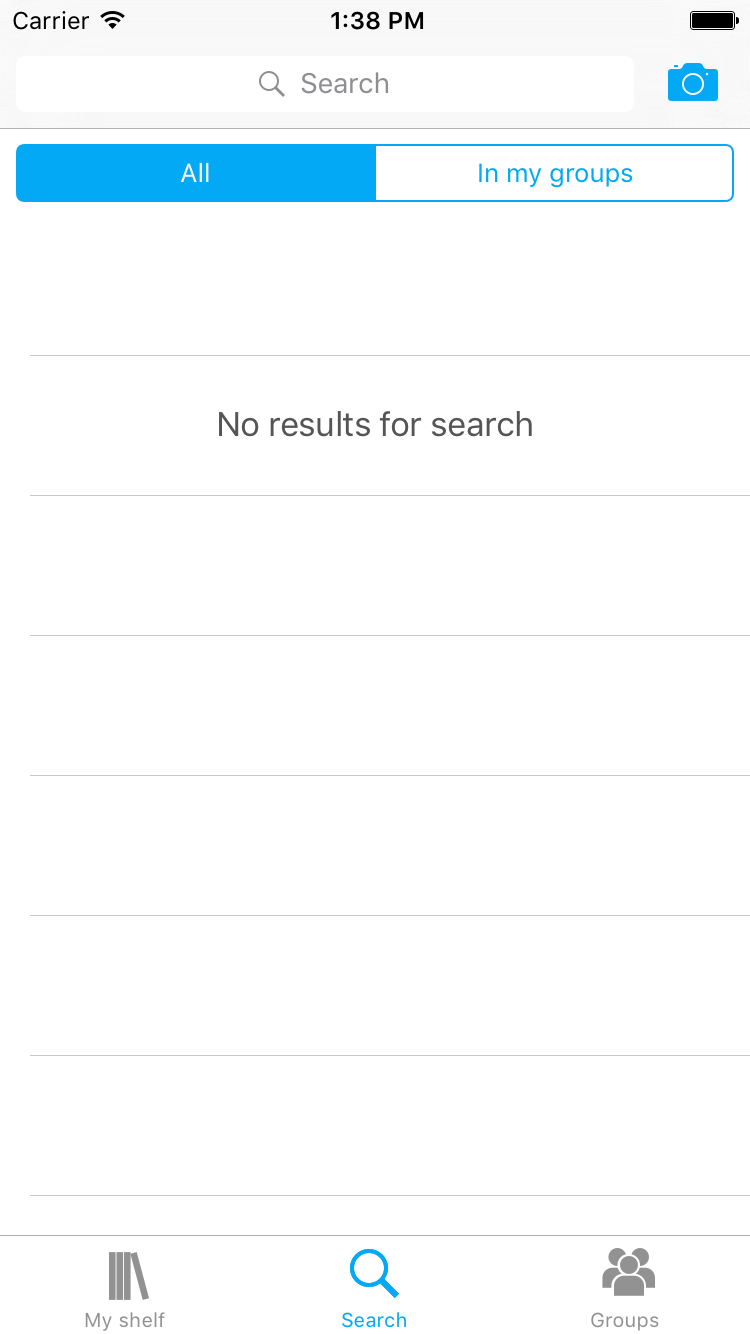
\includegraphics[width=.4\textwidth]{figs/v05/ios-search-view.png}
  \caption{Search empty view}
  \label{fig:ios-search-view-empty-5}
\end{subfigure}%
\begin{subfigure}{.5\textwidth}
  \centering
  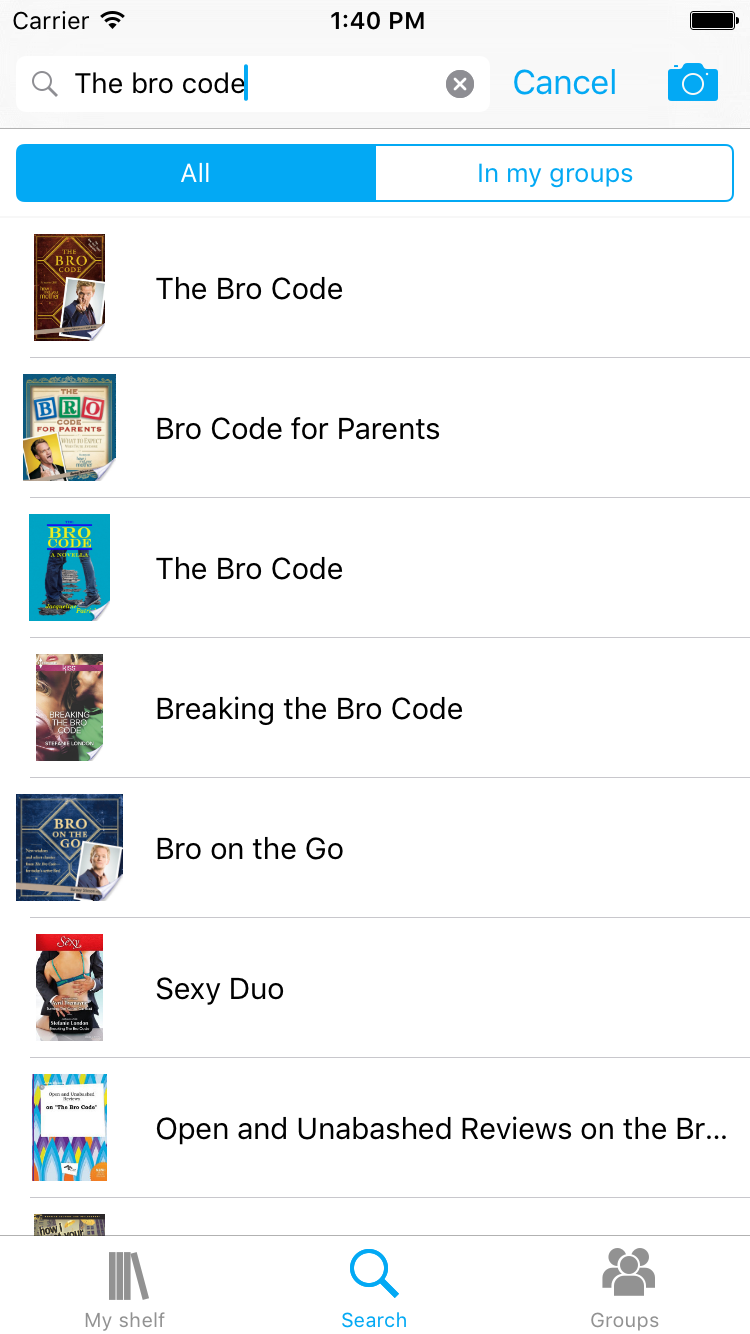
\includegraphics[width=.4\textwidth]{figs/v05/ios-search-results.png}
  \caption{Search view with results}
  \label{fig:ios-search-view-results-5}
\end{subfigure}
\caption{iOS search view design in version 0.5}
\label{fig:ios-search-view-5}
\end{figure}

\begin{figure}
\centering
\begin{subfigure}{.5\textwidth}
  \centering
  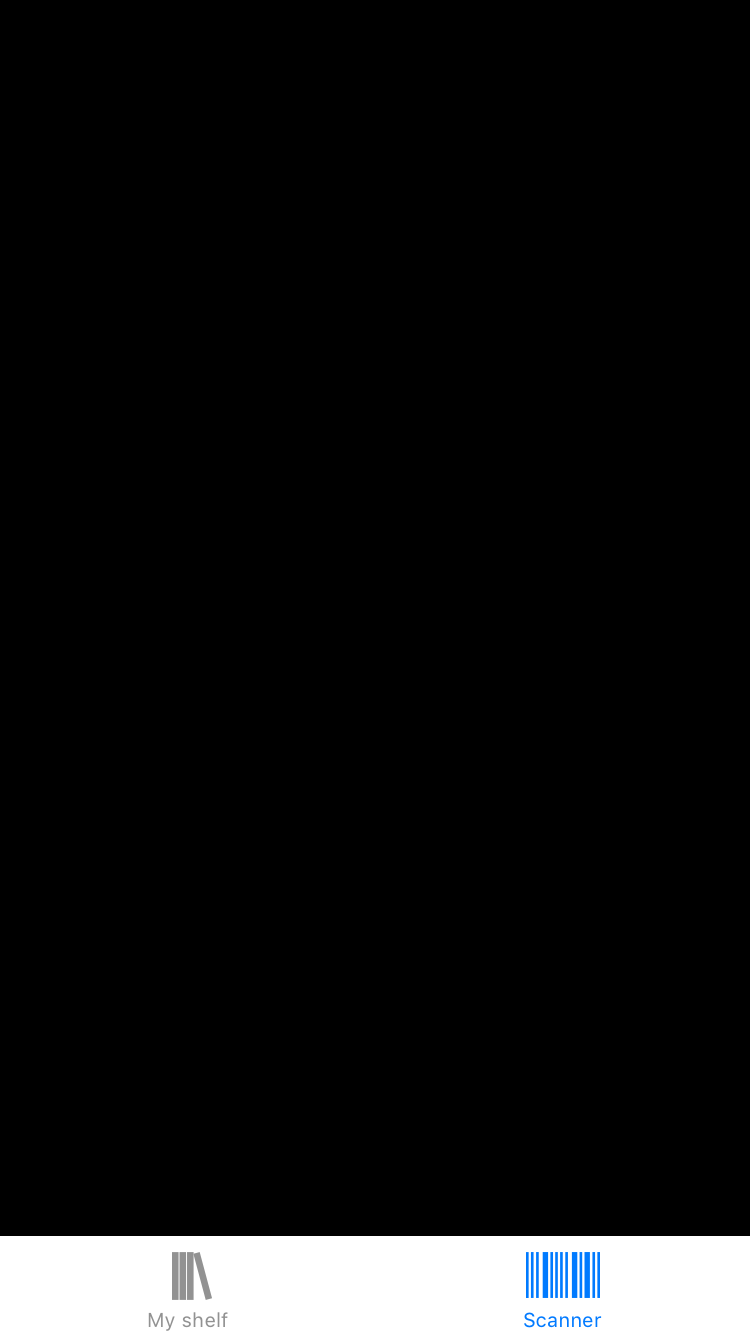
\includegraphics[width=.4\textwidth]{figs/v02/ios-scanner-view.png}
  \caption{Version 0.2}
  \label{fig:ios-scanner-view-2}
\end{subfigure}%
\begin{subfigure}{.5\textwidth}
  \centering
  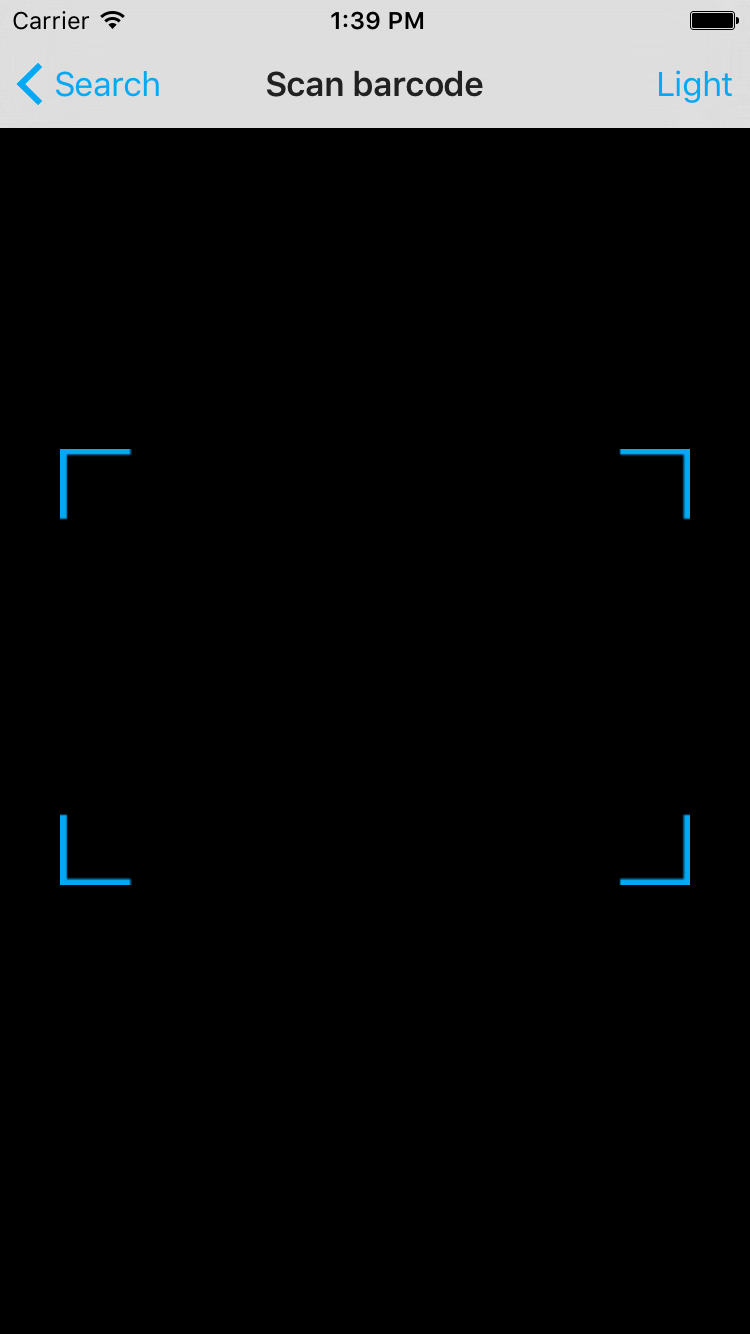
\includegraphics[width=.4\textwidth]{figs/v05/ios-scanner-view.png}
  \caption{Version 0.5}
  \label{fig:ios-scanner-view-results-5}
\end{subfigure}
\caption{Comparison of the old and new scanner design}
\label{fig:ios-scanner-view-comparison-5}
\end{figure}


    \item[Feedback] \hfill\\
The integration of Mixpanel from version 0.5 was extended to also include reporting the users search activity. This would allow the team to monitor how the new features were used.
\end{description}

\subsubsection{Backend}
For this iteration the \gls{backend} team was given the task of developing a full user service, as well as the possibility for the system to send e-mails, retrieve lost passwords and invite friends. In addition, the user stories from this iteration as well as the earlier ones, indicated that the team would need to develop a way for the users to authorize themselves, so that not all users could do all operations. Because all this had to be one huge update of the \gls{API}, the team decided to move the release of these features to version 0.6. See section \ref{v06-backend}.


\subsection{Feedback}
In answering the questions to confirm the assumption of this version the success was not satisfactory. The application was released containing the Mixpanel tracking to measure the use of both search and what result the users wanted, but there was not enough user data after version 0.5 was released to be able to say that the assumption was correct. On the other hand it did not imply that it was not correct either. Due to this, the feature was kept, but not improved until more feedback was received.

Even though the application received only a small amount of feedback, the customer representative had stated that both search and user validation was desired as mentioned in the planning section. Therefore, despite the lack of feedback from other users, the team could continue with implementing version 0.6.

\subsection{Version progress}
As shown in figure \ref{fig:version-progress-5} this version started on a Thursday, and the team did get to real work before the weekend was over. After that the progress was nice and steady, of course there was some differs in the number of tasks completed each day, but, this is because some of the tasks took longer to complete.

During this version the team really felt they had started to get a hang of the technical part of the project. The version was completed within the time limit, which was not that long, and the team did not encounter any major problems during the implementation. The blog posts describing this version are found in figures \ref{fig:week-nine} and \ref{fig:week-ten}

The tasks completed during version 0.5 are found in appendix \ref{app:release-note-5} including the user stories that the tasks were based upon. 

\begin{figure}
\centering
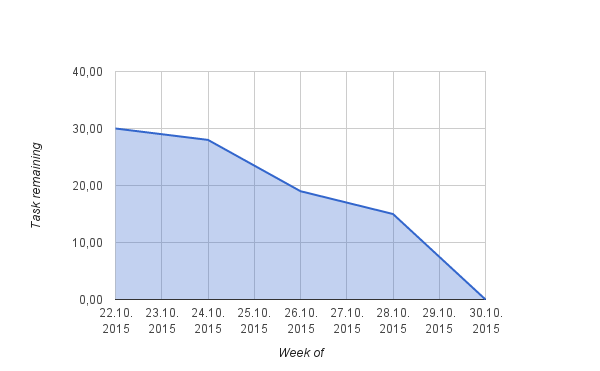
\includegraphics[height=10cm]{figs/v05/version-progress-5.png}
\caption{Task progress version 0.5}
\label{fig:version-progress-5}
\end{figure}

\begin{figure}
\centering
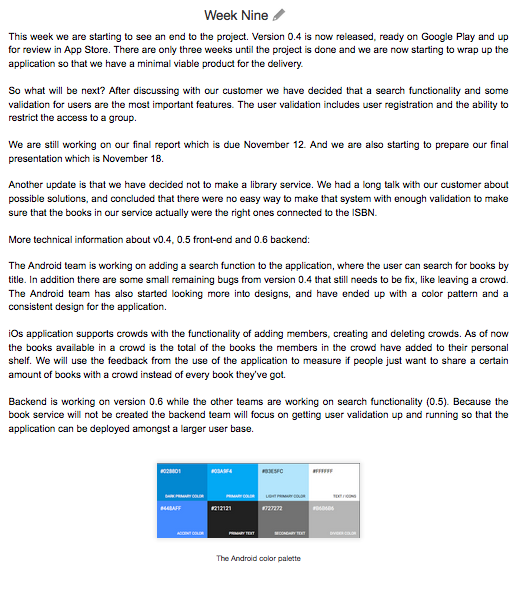
\includegraphics[height=17cm]{figs/v05/weekNine.png}
\caption{Blog post from week nine}
\label{fig:week-nine}
\end{figure}

\begin{figure}
\centering
\includegraphics[height=20cm]{figs/v05/weekTen.png}
\caption{Blog post from week ten}
\label{fig:week-ten}
\end{figure}



\subsection{Review and retrospective}
Between version 0.5 and 0.6 the team did not have a customer meeting with the customer representative due to his job taking up most of that week. However, the customer representative had in the previous meeting told the team what was needed to create a \gls{MVP} and the team could therefore continue with the next version of the application.

After version 0.5 was complete the team had an internal retrospective meeting to discuss to progress and atmosphere of the project. The whiteboard with the opinions is shown in figure \ref{fig:retrospective-5}.
\begin{figure}
\centering
\includegraphics[height=10cm]{figs/v05/retrospective-5.JPG}
\caption{The whiteboard after the retrospective meeting of version 0.5}
\label{fig:retrospective-5}
\end{figure}

In this meeting there was a lot of positive feedback from the group. Some key points that went well this version was the smooth implementation of the product and especially the Android development that in earlier versions has taken a lot more time. Other than that there were mentions of good communication, quick response time, and a lot of initiative.

The improvement list has been shortened a lot since the first group retrospective meeting, but there are still some point to get better. First it is the synchronization of design on the two platforms which was mentioned at the last retrospective as well. The team has started to work on that. Other point were focusing on the essential tasks, not all the possible improvements, and get better at moving completed tasks to the Done-column in JIRA. The two things that were noticed by most of the members was the lack of report writing and the continuous documentation of the software being made. These points were selected as focus for version 0.6


\subsection{Summary}
During this version the design of both mobile application was updated. Search functionality was implemented in the mobile applications while the backend team worked on supporting user validation in parallel with fixing bugs that the mobile developers found when implementing their functionality. 

After discussing with the customer representative the team will develop version 0.6 that support of user validation and the application will then be distributed to employees at Netlight. 

\section{Version 0.6}
\subsection{Assumptions and questions}
The assumption to be confirmed or refuted in this version is "Users want to limit the accessibility to their crowds"

Questions needed to decide whether the assumption is valid or not are:

\begin{enumerate}
    \item To what extent do they want the other users to be authenticated?
    \item On what ground do they wish to limit the access?
\end{enumerate}
    
\subsection{Planning and design}

The customer representative had already stated that user authentication was necessary to achieve a \gls{MVP}. Therefore the team could begin implementing the necessary changes needed in the applications to support this feature. The first task was to design a new sign in view and register view. Due to limited time, it was decided that there was no time for usability testing. The new design was therefore heavily based on Facebook's design of equivalent views, based on the assumption that Facebook have conducted the necessary usability tests.


\begin{figure}
\centering
\includegraphics[height=7cm,angle=-90]{figs/v06/signin-whiteboard.jpg}
\caption{Design sketch from the planning phase}
\label{fig:design-sketch-6}
\end{figure}

\begin{figure}
\centering
\begin{subfigure}{.5\textwidth}
  \centering
  \includegraphics[width=.4\textwidth]{figs/v06/facebook-login-view-6.png}
  \caption{The Facebook login view}
  \label{fig:facebook-login-view-6}
\end{subfigure}%
\begin{subfigure}{.5\textwidth}
  \centering
  \includegraphics[width=.4\textwidth]{figs/v06/crowdshelf-login-view-6.png}
  \caption{The CrowdShelf sign in view}
  \label{fig:crowdshelf-login-view-6}
\end{subfigure}
\caption{Comparison of the Facebook login and CrowdShelf sign in design}
\label{fig:login-view-comparison-6}
\end{figure}


The customer representative also requested an email explaining the concept of the application, who the team were, and how to install the application, which he could send to his colleagues in Netlight to deploy the application.


\subsection{User stories}
\label{user-stories-v6}
These user stories were selected to describe the functionality of version 0.6.
\begin{enumerate}
    \item As a USER I want to be the only one who can edit My Shelf
    \item As a USER I want a secure authentication
\end{enumerate}

\subsection{Development}
This section describes what was developed during this version.

\subsubsection{Backend}
\label{v06-backend}
In this iteration the team wanted to finalize the \gls{backend} solution, and the results here is the result of both this iteration, and version 0.5. The reason for this was that the features had to be rolled out at once, as they were so tightly coupled. 

The iterations included complete user support, log-in and authorization. To be able to let user reset passwords and do similar operations, the team agreed that one would want the server to be able to send e-mails, so the iterations started by writing a general e-mail module within the server. The module provided a way to send an e-mail to send an e-mail to a list of addresses with a simple function call. The team then added templates for the different e-mails that had to be sent, and a helper-module that could handle building clean HTML- or text-documents, with user specific details. To accomplish this, the team used third party libraries. \cite{nodemailer}

When the e-mail service was ready, the team continued with updating the user model. This meant adding a password-field to the validation of user objects. The password had to be hashed, which was implemented with bcrypt. \cite{bcrypt} The login-request was also extended with a password-field, which was validated to be correct or not with the same bcrypt-library. If the login information was valid, the server was made to respond with the user object and a token. The token was generated with a library called Hat, and then added to a MonogDB-collection together with a expiration date 20 minutes ahead in time. \cite{hat} All requests that were not related to retrieving lost passwords, logging in or creating a new user now demanded a valid token. After 20 minutes the user had to login again. The login information could be saved locally in client application.

The team had a long discussion on how the authorization should be implemented. \gls{HTTPS}-certificates can be expensive, so it was not possible to use any real encryption. The team found that the token-strategy with a very limited time frame would be sufficient at this point, but that all connections should be encrypted if that could ever be a real option.

\subsubsection{Android}
\begin{description}
    \item[Features] \hfill\\
    \label{para:androidFeature06}
% Locally store token
The main focus for version 0.6 was authentication of the user in the application. This included only allowing changes to a user or a crowd if you have access to that specific user. This was implemented by demanding the user to enter both username and password when signing in. To be able to implement this feature the team also needed to add the possibility to create a user with a password. This was done by adding an extra text field to the create user screen, and including the user's input when sending data to the \gls{backend}. 

Since there is a possibility that the user can forget the password to their account. The team also implemented a feature for resetting a user's password. This was done by adding a new screen where a user could input a username. The \gls{backend} would then use this username to send an email to the user's email address. This email will contain a key the user needs to input into the application along with a new password. 

The last important feature for this version is that the team changed how the user uses the scanner. Before this version the user had to swipe or use the tabbed navigation bar at the top of the main screen to change to the scanner screen. In this version a new button was added at the top right of the screen. This button opened a new activity which used the camera of the device. This allowed the team to open the scanner from anywhere in the application. 

    \item[Structure] \hfill\\
Figure \ref{fig:AndroidStructure-06} shows the structure of the Android application after the features of version 0.6 was implemented. The most important activities for this version are the \code{ForgotPasswordAcitivty} activity which handles the resetting of a user's password and the \code{ScannerCaptureActivity} activity. The \code{ScannerCaptureActivity} activity is handling the scanning of barcode using the camera of the device and returning the barcode number to the \code{MainTabbedAcitivy} activity.

\begin{figure}
\centering
\includegraphics[width=\textwidth]{figs/v06/Android/AndroidStructure-06.png}
\caption{Android version 0.6 structure}
\label{fig:AndroidStructure-06}
\end{figure}

    \item[Design] \hfill\\
The main design change in version 0.6 is a result of the change in the scanner functionality. Because the scanner no longer is implemented in the application as a fragment it could no longer be a part of the tabs in the \code{MainTabbedActivity} activity. This is illustrated in figure \ref{fig:androidcompareDesign05}. Figure \ref{fig:androidcompareDesign06} shows how the scanner functionality is replaced in version 0.6. It is now a button in the top right of the screen opening a scanner view with the same functionality as in previous versions. Another design change that was made was to include a back button on some activities as a result of feedback from our users, this can be seen in figure \ref{fig:AndroidBackButton}

\begin{figure}
\centering
\begin{subfigure}{.5\textwidth}
  \centering
  \includegraphics[width=.8\textwidth]{figs/v05/AndroidDesign-05.png}
  \caption{Version 0.5}
  \label{fig:androidcompareDesign05}
\end{subfigure}%
\begin{subfigure}{.5\textwidth}
  \centering
  \includegraphics[width=.8\textwidth]{figs/v06/Android/AndroidDesign-06.png}
  \caption{Version 0.6}
  \label{fig:androidcompareDesign06}
\end{subfigure}
\caption{Android design changes from version 0.5 to version 0.6}
\label{fig:AndroidDesignComparison06}
\end{figure}

    \item[Bug fixes] \hfill\\
In version 0.5 the views for creating groups and editing existing groups used the same activity. This caused a bug that none of the buttons were hidden, which meant that buttons only relevant for existing groups were shown when creating a new group. If some of these buttons were clicked before the group was created it would result in an error. The solution to this bug was to make the buttons invisible if they were unusable for the current state of the view. 

Some minor bugs were also resolved. In previous versions it was not possible to create a group without any members. This functionality was desired when some users who tried to first create an empty group before later adding members.

As described in the Android feature paragraph the scanner as a fragment was removed from the \code{MainTabbedActivity} activity and rather used as an activity, the \code{ScannerCaptureActivity}. Previous to version 0.6 the application ran slow on some devices since the camera of the device were running continuously in the background. This was a result from having the scanner as a fragment. When changing the scanner feature to an activity it resulted in an improvement in the performance of the application.

\begin{figure}
\centering
\includegraphics[height=2cm]{figs/v06/backArrow.png}
\caption{The back arrow in action bar}
\label{fig:AndroidBackButton}
\end{figure}

\end{description}

\subsubsection{iOS}
\begin{description}
    \item[Features] \hfill\\
The new features in this version was a new register view, an updated login view, and user authentication. The new two views were meant to updated according to the design sketch, but there were not enough time to complete the task. To enable user authentication, the sign in procedure had to be updated in order to accept and store the new token received from the CrowdShelf \gls{backend}. This token had to be sent as a parameter in all requests to the server to verify that the user should have access to the data. This was fully implemented before the development ended, but a few issues with the server prevents the system from being fully operational.  

    \item[Design] \hfill\\
Apart from the uncompleted registration view, there were no major changes this version. The main difference was that the theme color was changed from Apple's default darker blue, to CrowdShelf's happier and lighter blue.


    \item[Feedback] \hfill\\
Due to the short time available for this version, the implementation was not completed, and therefore there is no feedback from usage of the applications or \gls{backend}. If there had been more time available, the clients and server would have been completed and distributed as a \gls{MVP} to Netlight. Then usage data could have been collected using Mixpanel in order to evaluate how the users adopt the new technology.

Unfortunately, there was not enough time to write the email to Netlight's employees either. This could have provided the users needed for the learning process.
\end{description}


\subsection{Version progress}
Because the \gls{backend} team had been working on user authentication during version 0.5, the velocity of the development on the clients was quite good. User authentication, email services and the updated login procedure was quickly added to the \gls{backend}, but a few bugs on both clients and the \gls{backend} caused the velocity to decrease. During the meeting with the customer representative \ref{app:customer-minutes-10} it was decided that the development should come to an end. Thus both applications were only partially functional and contained multiple bugs.

A blog post from the end of this version can be seen in figure \ref{fig:blog-week-11}. 

\begin{figure}
\centering
\includegraphics[height=\textheight]{figs/v06/week-11.png}
\caption{Blog post from week eleven}
\label{fig:blog-week-11}
\end{figure}

\subsection{Review}
After discussing with the customer representative it was decided that the implementation should be stopped to focus on the report. That decision made this the last version of the application. The result of this version which also is the final product of the application is concluded in the next section. 


\subsection{Summary}
As a summary of this version, the team started with the plan of implementing user authentication, and this feature was created. A consequence of the abrupt stop of implementation was that the last version contains many bugs. These bugs will be fixed after the report is delivered.

With version 0.6 complete the development part of the project is completed. Table \ref{version-schedule} lists all the versions completed with release dates and functionality included. Chapter \ref{chap:ArchitecturalDescription} includes a complete overview of the system architecture. A summary of the functionality in the applications and \gls{API} is described in section \ref{conclusion-system-overview}.

\begin{table}[]
\centering

\begin{tabular}{|L{3cm}|L{3cm}|L{8cm}|}
\hline
\textbf{Version} & \textbf{Release date} & \textbf{Description} \\
\hline
0.1 & 20/Sep/15 & This version produced two videos created to explain the product, and test the markets interest. \\
\hline
0.2 & 25/Sep/15 & A user has the possibility to view their books, scan the books barcode using the phones camera and add or remove those books. \\
\hline
0.3 & 07/Oct/15 & This version includes the feature of borrowing and returning books. The borrowed and lent out books are shown in the shelf view. \\
\hline
0.4 & 21/Oct/15 & This version includes group functionality, a way to find out what books users you know, or just want to share books with owns. \\
\hline
0.5 & 29/Oct/15 & In this version the possibility to search for books is included. A user can search globally of locally in their groups. \\
\hline
0.6 & 06/Nov/15 & This version has updated the login functionality by adding user validation.\\
\hline
\end{tabular}
\caption{Schedule of versions}
\label{version-schedule}
\end{table}



